% ---------------
% PREAMBLE
% ---------------
\newif\iflatextortf

\iflatextortf
	% tell latex2tortf if this is an article or report
 	\documentclass[12pt,letterpaper]{article}
	\input{NRELLatex2rtf.tex}
\else
	%\documentclass[report,tagged]{nrel}
	\documentclass[report]{nrel}
\fi

% -----------------------------------
% DOCUMENT PROPERTIES
% -----------------------------------
\title{SAM Photovoltaic Model Technical Reference}
\author{Paul Gilman, Aron Dobos, Nicholas DiOrio, Janine Freeman, Steven Janzou, David Ryberg}


% -----------------------------------
% DOCUMENT PROPERTIES
% -----------------------------------
\usepackage{array}
\usepackage{dcolumn}
\newcolumntype{.}{D{.}{.}{2.7}}

% -----------------------------------
% MULTI-LETTER VARIABLE NAMES
% -----------------------------------
\newcommand\GCR{\ensuremath{\mathit{GCR}}}
\newcommand\AOI{\ensuremath{\mathit{AOI}}}

% -----------------------------------
% DIRECTORIES
% -----------------------------------
\graphicspath{{figures/}}

% -----------------------------------
% START DOCUMENT
% -----------------------------------
\begin{document}

%%%%%%%%%%%%%%%%%%%%%%%%%%%%%%%%%%%%%%%%%%%%%%%%%%
%%%%%%%%%%%%%%%%%%%%%%%%%%%%%%%%%%%%%%%%%%%%%%%%%%
\frontmatter
\chapter*{Executive Summary}

This manual describes the photovoltaic performance model in the System Advisor Model (SAM). The U.S. Department of Energy's National Renewable Energy Laboratory maintains and distributes SAM, which is available as a free download from \url{https://sam.nrel.gov}. These descriptions are based on SAM 2015.1.30 (SSC 41).

SAM is a techno-economic feasibility model for renewable energy projects. It is designed for a range of different users, including project developers, system designers, policy makers, financial planners, and academic researchers.

SAM's photovoltaic performance model is available both as part of the SAM desktop application, and in the SAM software development kit (SDK). This manual is intended for people who want to understand SAM's photovoltaic model, or for people who are using the SDK to develop their own applications.

SAM runs on Windows and OS X operating systems, and is a user interface that performs the following functions:

\begin{itemize}
\item Organizes and displays the performance and financial model inputs in a user-friendly interface.
\item Manages tasks associated with running model simulations.
\item Provides options for ``advanced" simulations that involve multiple simulation runs for parametric and sensitivity studies.
\item Stores arrays of model results.
\item Calculates secondary results such as monthly and annual totals, capacity factor, system performance factor, and system losses.
\item Displays tables and graphs of results.
\item Allows for exporting data in different formats, CSV, graph images, Microsoft Excel, and a PDF report.
\end{itemize}

The SAM SDK is a package containing the SAM Simulation Core (SSC) libraries and a set of software development tools that allow model developers to create their own interfaces to the simulation modules as either web or desktop applications.

%%%%%%%%%%%%%%%%%%%%%%%%%%%%%%%%%%%%%%%%%%%%%%%%%%
%%%%%%%%%%%%%%%%%%%%%%%%%%%%%%%%%%%%%%%%%%%%%%%%%%
\mainmatter
\tableofcontents
\listoffigures
\listoftables

%%%%%%%%%%%%%%%%%%%%%%%%%%%%%%%%%%%%%%%%%%%%%%%%%%
%%%%%%%%%%%%%%%%%%%%%%%%%%%%%%%%%%%%%%%%%%%%%%%%%%
\chapter{Nomenclature}

The organization of this manual is based roughly on the Sandia National Laboratories PV Performance Modeling Collaborative (PVPMC) website ``Modeling Steps" \citep{pvpmc}. The nomenclature and general descriptions also draw from the ``PVCDROM" electronic document on the pveducation.org website hosted by the Arizona State University Solar Power Labs \citep{pvcdrom}.

The variable names in this manual are listed in tables at the beginning of each section. In some cases, the same variable name might be used in two different sections of the manual to represent two different quantities. That is because we have tried to preserve the variable names used in the original sources. For example, $E$ is used to represent solar irradiance in most equations, and for the band-gap energy in two equations in the Sandia module model section.

For solar irradiance values, the letter $E$ indicates data from the weather file, $I$ indicates irradiance incident on the photovoltaic array before soiling and shading, and $G$ indicates effective irradiance incident on the array (at the top of the module cover) after soiling and shading. The subscripts $b$, $d$, and $g$ indicate beam, diffuse, and global irradiance values.

The variable $P$ indicates an electrical power value in Watts or kilowatts. Because SAM is an hourly simulation model, these power values are average hourly values, equivalent to Watt-hour (or kilowatt-hour) per hour.

%%%%%%%%%%%%%%%%%%%%%%%%%%%%%%%%%%%%%%%%%%%%%%%%%%
%%%%%%%%%%%%%%%%%%%%%%%%%%%%%%%%%%%%%%%%%%%%%%%%%%
\chapter{Photovoltaic Performance Model Overview}

SAM's photovoltaic performance model combines module and inverter submodels (see Table~\ref{tab-submodels}) with supplementary code to calculate a photovoltaic power system's hourly AC output given a weather file and data describing the physical characteristics of the module, inverter, and array. The main submodels are listed in Table~\ref{tab-submodels} with a citation of the publication that originally described the modeling approach or an indication that the submodel uses standard equations, or was developed by the National Renewable Energy Laboratory (NREL), in which case the description in this manual is the only documentation of the modeling approach.

\begin{table}
\begin{center}
\caption{The Primary SAM Photovoltaic Performance Model Submodels}
\begin{tabular}{ll}
\midrule
Submodel & Reference\\
\midrule
Weather file reader & NREL\\
Sun position & \citet{michalsky1988}, \citet{iqbal1983}, NREL\\
Surface angles & standard geometry\\
Backtracking for one-axis trackers & NREL\\
Isotropic incident irradiance model & \citet{liu1963}\\
HDKR incident irradiance model & \citet{duffie2013}, \citet{reindl1988}\\
Perez 1990 incident irradiance model & \citet{perez1988}, \citet{perez1990}\\
Self shading model for fixed arrays & \citet{deline2013a}\\
Self shading model for one-axis trackers & NREL \\
Sandia module model & \citet{king2004}\\
CEC module model & \citet{desoto2004a}\\
Simple efficiency module model & NREL\\
Subarray mismatch calculator & NREL \\
Sandia inverter model & \citet{king2007}\\
Part load inverter model & NREL\\
\hline
\end{tabular}
\label{tab-submodels}
\end{center}
\end{table}


The photovoltaic performance model can simulate any size of system, from a small rooftop array and a single inverter to a large system with multiple subarrays and banks of inverters.

The model calculates the system's AC electrical output over one year as an array of 8,760 hourly AC power values. It reads hourly solar resource and temperature data from a weather file describing the resource at the system's location for the year, and uses them with inputs describing the system's design in equations to calculate module and inverter conversion efficiencies and energy losses.

The modeled system must consist of a single type of photovoltaic module and a single type of inverter -- it cannot combine different sizes or brands of modules and inverters. The array may consist of up to four subarrays, each with its own set of parameters for tracking, surface angles, shading and soiling, and DC losses. Each subarray can have a different number of modules, but all subarrays must have the same number of modules per string so that all subarrays have the same nominal DC voltage, which serves as the inverter's nominal input voltage.

The array must be connected either to a single inverter or to a bank of inverters connected to each other in parallel. It is not possible to model a system with subarrays connected to different inverters.

The module model (Section~\ref{sec-module}) and inverter model (Section~\ref{sec-inverter}) calculate solar-energy-to-DC-electricity and DC-to-AC electricity conversion efficiencies, respectively, and account for losses associated with each component. The self-shading models (Section~\ref{sec-selfshad}) calculate losses caused by shading of modules in the array by neighboring modules. The photovoltaic performance model does not explicitly calculate the remaining system losses. They are represented by user-specified inputs:

\begin{itemize}
\item{Beam and diffuse shading losses for near-object shading of the array (Section~\ref{sec-nearobjectshad}). These can be specified as hourly (8,760 values), month-by-hour (288 values), or sun azimuth angle by elevation (number of values varies), and may be generated by shading analysis equipment and software.}
\item{Monthly soiling losses for dust and other accumulation on the array (Section~\ref{sec-soiling}).}
\item{DC losses for module mismatch, DC wiring and connections, tracking, and other losses associated with the array (Section~\ref{sec-dclosses}).}
\item{AC losses for AC wiring and transformer losses (Section~\ref{sec-aclosses}).}
\end{itemize}

The photovoltaic model uses the same algorithm to calculate self-shading losses for fixed arrays and one-axis trackers (Section~\ref{sec-selfshad}). It does not calculate self-shading losses for two-axis or azimuth-axis trackers. The self-shading algorithm calculates a reduction in diffuse POA irradiance and a DC loss factor to account for the performance impact of the reduction in beam POA irradiance.

The model does not calculate module mismatch losses within a subarray. For systems with more than one subarray, an optional algorithm can estimate mismatch losses between the subarrays (Section~\ref{sec-mismatch}).

\section{Model Algorithm}

This section describes the basic algorithm of SAM's photovoltaic performance model. The details of each step listed below are described in the sections that follow. See Figure~\ref{fig-pvsamschematic} for a basic block diagram of the model. Note that the block diagram does not include the subarray mismatch and string voltage calculations described in the steps below to make the diagram easier to follow.

\begin{figure}
\begin{center}
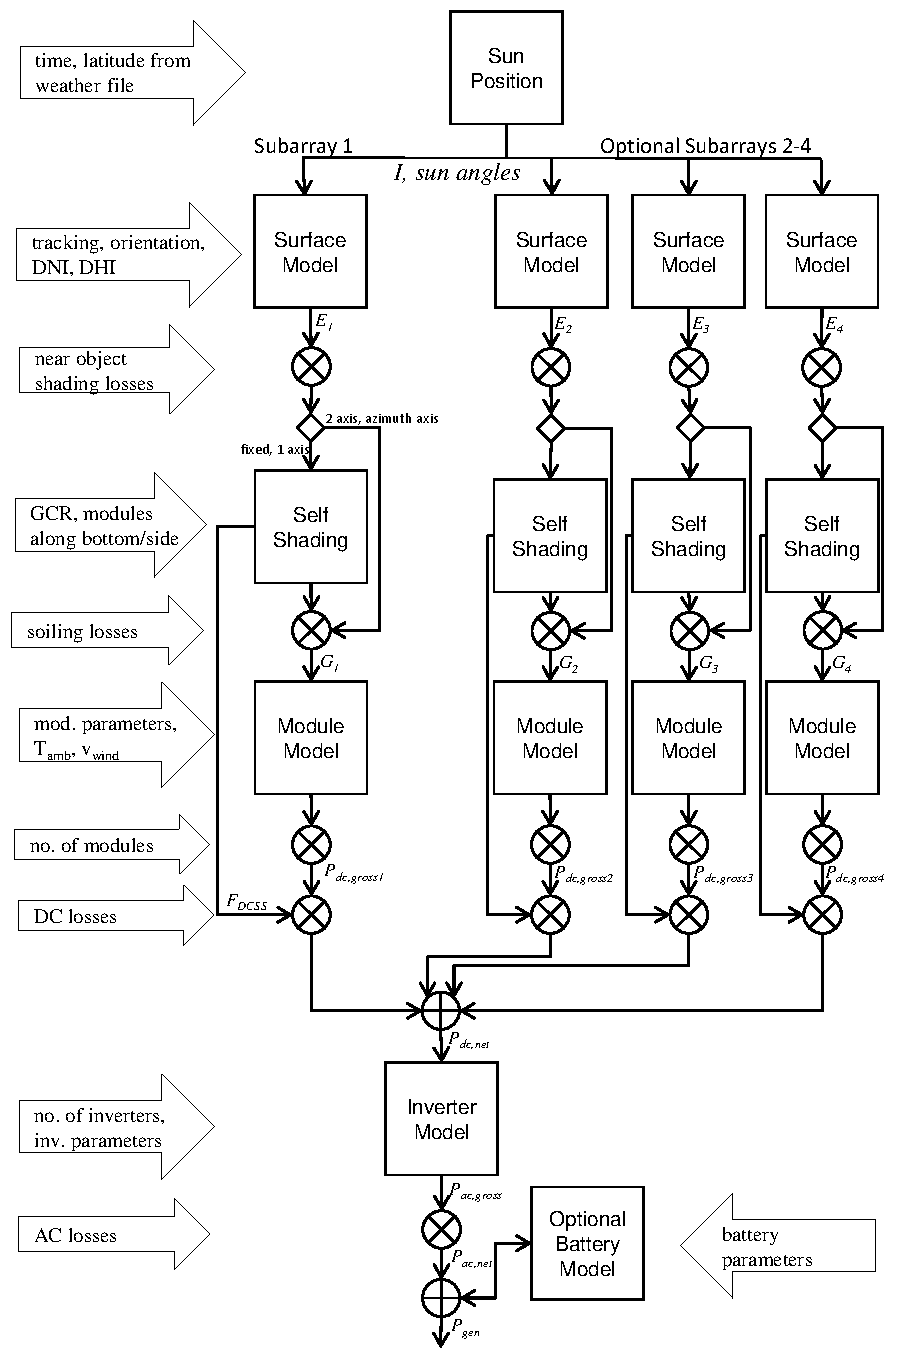
\includegraphics[scale=0.88]{pvsam-schematic}
\caption{Photovoltaic Performance Model Simplified Block Diagram}
\label{fig-pvsamschematic}
\end{center}
\end{figure}
 
The hourly simulation model performs the following calculations for each of the 8,760 hours in a year:

\begin{enumerate}

\item{For each of up to four subarrays:}

  \begin{enumerate}

  \item{Calculate sun angles from date, time, and geographic position data from the weather file. (Section~\ref{sec-sunangles})} %irrad.calc() called from cmod_pvsamv1.cpp 1213 from inside subarray loop. solarpos() called in irrad.calc() lib_irradproc.cpp 855 etc

  \item{Calculate the nominal beam and diffuse irradiance incident on the plane of array (POA irradiance). This depends on the solar irradiance data in the weather file, sun angle calculations, user-specified subarray parameters such as tracking and orientation parameters, and backtracking option for one-axis trackers. (Section~\ref{sec-nominalincidentirradiance})} %irrad.calc() called as above. incidence() called in irrad.calc() lib_irradproc.cpp 900 etc

  \item{Apply the user-specified beam and diffuse near-object shading factors to the nominal POA irradiance. (Section~\ref{sec-nearobjectshad})} %cmod_pvsamv1.cpp 1235-1249

  \item{For subarrays with one-axis tracking and self-shading enabled, calculate and apply the self-shading loss factors to the nominal POA beam and diffuse irradiance. (Section~\ref{sec-selfshad})} %cmod_pvsamv1.cpp 1254 call shade_fraction_1x() in lib_irradproc.cpp for beam shading loss, 1259-1318 for sky and ground diffuse factors

  \item{Apply user-specified monthly soiling factors to calculate the effective POA irradiance on the subarray. (Section~\ref{sec-soiling})} %cmod_pvsamv1.cpp 1328

  %\item{Record subarray outputs.} %cmod_pvsamv1.cpp 1338

  \end{enumerate}

\item{If there is a single subarray (Subarray 1) with no tracking (fixed) and self-shading is enabled, calculate the reduced diffuse POA irradiance and self-shading DC loss factor. (Section~\ref{sec-selfshadalg})} %sscalc.exec() called in cmod_pvsamv1 1378

\item{Determine subarray string voltage calculation method (Section~\ref{sec-dcstringvoltage}).} \label{item-mismatch} %cmod_pvsamv1.cpp 1403

\item{For each of up to four subarrays, run the module model with the effective beam and diffuse POA irradiance and module parameters as input to calculate the DC output power, module efficiency, DC voltage, and cell temperature of a single module in the subarray.} %call pvinput_t in() and out() from lib_pvmodel.cpp to set inputs and outputs cmod_pvsamv1.cpp 1459, then run module model 1471

\item{Calculate the subarray string voltage using the method determined in Step \ref{item-mismatch}.} %lib_pvsamv1.cpp 1486

\item{Loop through the subarrays to calculate the array DC power (Section~\ref{sec-arraydcoutput}):} %lib_pvsamv1.cpp 1491

  \begin{enumerate}

  \item{For Subarray 1, apply the fixed self-shading DC loss to the module DC power if it applies.} %lib_pvsamv1.cpp 1498

  \item{For each subarray, calculate the subarray gross DC power by multiplying the module DC power by the number of modules in the subarray.} %lib_pvsamv1.cpp 1502

  \item{For each subarray, calculate subarray net DC power by multiplying the gross subarray power by the DC loss.} %lib_pvsamv1.cpp 1505

  \item{For each subarray, calculate the subarray string voltage by multiplying the module voltage by the number of modules per string.} %lib_pvsamv1.cpp 1511

  \item{Calculate the array net and gross DC power by adding up the subarray values.}

  \end{enumerate}

\item{Run the inverter submodel to calculate the gross AC power and inverter conversion efficiency (Section~\ref{sec-inverter}).} %lib_pvsamv1.cpp 1515

%\item{Calculate irradiance values for results} %lib_pvsamv1.cpp 1535

\item{Calculate the net AC power by applying the AC loss to the gross AC power. (Section~\ref{sec-netacoutput})} %lib_pvsamv1.cpp 1570

\end{enumerate}

\section{Component Libraries and Weather Files} \label{sec-libraries}

SAM includes a set of component libraries and weather files that store copies of data managed by different organizations. The component libraries store module and inverter parameters that represent the components' physical properties. The weather files store data representing the solar resource at different locations.

The following is a list of the databases used by SAM's photovoltaic performance model:
\begin{itemize}
\item California Energy Commission Eligible Photovoltaic Modules \citep{gsc2014b}
\item California Energy Commission Eligible Inverters \citep{gsc2014c}
\item Sandia National Laboratories Module Database \citep{sandia-testeval}
\item NREL National Solar Radiation Database 1961-1990 (TMY2) \citep{nsrdb}
\item NREL National Solar Radiation Database 1991-2010 Update (TMY3) \citep{nsrdb}
\item U.S. DOE EnergyPlus Weather Data \citep{epw}
\item NREL Solar Prospector \citep{solarprospector}
\end{itemize}

Note that these data collections are not part of SSC. If you are developing a model using the SAM software development kit and want to use the component libraries, you will have to write your own code to read the data. (You can use SAM's library editor to export data from the component libraries to a text file as described in \citet{help-libraries}.)

\section{System Sizing} \label{sec-sizing}

SAM's System Design input page has an option that automatically calculates the number of modules per string, number of parallel strings in the array, and number of inverters given a desired array size in DC kW and a DC-to-AC nameplate capacity ratio. The sizing algorithm is described in \citet{help-sizing} and uses the module and inverter reference parameters for the capacity calculations.

The system sizing algorithm is not available in SSC.

%%%%%%%%%%%%%%%%%%%%%%%%%%%%%%%%%%%%%%%%%%%%%%%%%%
%%%%%%%%%%%%%%%%%%%%%%%%%%%%%%%%%%%%%%%%%%%%%%%%%%
\chapter{Irradiance and Weather Data}\label{sec-irradianceweatherdata}

The photovoltaic performance model requires a weather file with data describing the solar radiation and weather observations at the system location. It uses location information and hourly time stamps to calculate hourly sun position angles (Section~\ref{sec-sunposition}),  and irradiance data to calculate hourly plane-of-array (POA) irradiance values (Section~\ref{sec-incidentirradiance}). The cell temperature submodel (Section~\ref{sec-celltempoptions}) uses ambient temperature and wind speed data to calculate the hourly photovoltaic cell temperature values.

SAM can read files in the formats listed below. For general descriptions of the formats, and references to more detailed documentation see \citep{help-weatherfileformats}.

\begin{itemize}
\item SAM CSV: Comma-separated text format developed by NREL for use with SAM.
\item TMY3: Comma-separated text format developed by NREL for the National Solar Radiation Database 1991-2010 update.
\item TMY2: Text format developed by NREL for the National Solar Radiation Database 1961 - 1990 data set.
\item EPW: Text format derived from the TMY2 format for the EnergyPlus building modeling software. 
\end{itemize}

SAM reads and stores the weather file data shown in Table~\ref{tab-wfdata}. It ignores any additional data elements that may be included in the different weather file formats. For example, it ignores the source and uncertainty flags in the TMY3 file format.

\begin{table}
\begin{center}
\caption{Weather Data}
\begin{tabular}{lll}
\midrule
Symbol & Field & Description\\
\midrule
\multicolumn{3}{c}{Metadata Location Description}\\
- & Location ID* & numerical identifier [\textit{722780}]\\
 - & City* & location name [\textit{``Phoenix Sky Harbor Intl Ap"}]\\
- & State* & two-letter state abbreviation [\textit{AZ}]\\
$\mathit{tz}$ &Time zone & hours W of GMT [\textit{-7.0}] \\
$\mathit{lat}$ & Latitude & decimal degree N of 0 [\textit{33.450}] \\
$\mathit{lon}$ & Longitude & decimal degree W of 0 [\textit{-11.983}]\\
$\mathit{elv}$ & Elevation & meters above sea level [\textit{337}]\\
\midrule
\multicolumn{3}{c}{Hourly Data Records}\\
$\mathit{yr}$& Year & typical year [\textit{1988}] \\
$\mathit{mo}$ & Month & typical month (1-12) \\
$\mathit{day}$ & Day & day of year (1-365) \\
$\mathit{hr}$ & Hour & hour of day (0-23) in local time \\
$\mathit{min}$ & Minute & minute past the hour (0-59) \\
$E_g$ & Global horizontal irradiance (Wh/m$^2$) & total radiation on a horizontal surface \\
$E_b$ & Direct normal irradiance (W/m$^2$) & direct radiation on a surface normal to the sun \\
$E_d$ & Diffuse horizontal irradiance (Wh/m$^2$) & radiation on a horizontal surface from the sky \\
$v_{wind}$ & Wind speed (m/s) & wind speed \\
-  & Wind direction* ($^{\circ}$E of N) & wind direction \\
$T_a$ & Dry bulb temperature ($^{\circ}$C) & ambient dry-bulb temperature \\
- & Wet bulb temp* ($^{\circ}$C) & ambient wet-bulb temperature \\
- & Dew point temp* ($^{\circ}$C) & ambient dew-point temperature \\
- & Relative humidity* (\%) &  relative humidity \\
- & Pressure* (mbar) & atmospheric pressure \\
$D_{snow}$ & Snow depth (cm) & depth of snow \\
$\mathit{\rho}$ & Ground reflectance & ground reflectance factor or albedo \\
\midrule
\multicolumn{3}{l}{\textit{Table Notes}}\\
\multicolumn{3}{l}{The photovoltaic model does not use fields marked (*), but they are required by the weather file reader.}\\
\multicolumn{3}{l}{The italicized values in brackets are examples from a TMY3 file's header.}\\
\end{tabular}
\label{tab-wfdata}
\end{center}
\end{table}

\section{Time Convention and Resolution}

The weather file contains one year of data. The number of data rows in the file determines the simulation time step. For example, a file with 8,760 rows of weather data (not including header rows) would result in an hourly simulation. A weather file for a 15-minute simulation time step should have 35,040 rows in addition to the header rows.

The first row of data in the weather file is for the first time step after midnight on January 1, local standard time. For hourly data, the first row is for the hour ending at 1 a.m. on January 1. For 15-minute data, the first row is for the quarter hour ending at 1:15 a.m. on January 1.

By default, SAM calculates the sun position for the mid-point of the time step. For example, for hourly data, SAM calculates the sun position for each hour at 30 minutes after the hour so that the sun position for the 10:00 a.m. hour would be its position at 10:30 a.m. However, if the weather file includes a Minute column, SAM will instead use the minute indicated to calculate each time step's solar position.

\section{Irradiance and Insolation}

%% Also address questions about spectrum and field of view

Solar irradiance is a measure of the instantaneous power from the sun on a surface over an area, typically given in the SI units of watts per square meter (W/m$^2$). In the weather files from the National Solar Radiation Database \citep{nsrdb}, each irradiance value is the total solar radiation in the 60 minutes ending at a given time step. These values represent the average solar power over a given hour in watt-hours per hour per square meter (Wh/h$\cdot$m$^2$). In SAM these values are expressed in the mathematically equivalent W/m$^2$ (or converted to kW/m$^2$).

The weather file stores hourly values for the three components of solar irradiance:

\begin{itemize}
\item The total solar irradiance on a surface parallel to the ground (horizontal), called global horizontal irradiance.
\item The portion of the solar irradiance that reaches a surface normal to the sun in a direct line from the solar disk (typically assuming a measurement device with a $5^{\circ}$ field of view), called beam normal or direct normal irradiance.
\item The solar irradiance on a horizontal surface from the sky excluding the solar disc, or diffuse horizontal irradiance.
\end{itemize}

Insolation is a measure of the energy from the sun over a given time on a surface given in watt-hours per square meter (Wh/m$^2$). SAM calculates the monthly and annual insolation incident on the plane of the photovoltaic array (Section~\ref{sec-incidentirradiance}). 

\section{Weather Observations}

SAM uses ambient temperature and wind speed data from the weather file to estimate the effect of photovoltaic cell temperature on the array's performance. Although wind direction does have an effect on cell temperature, the photovoltaic performance model assumes that its cumulative effect over the year is negligible \citep{king2004}.

The air temperature or dry-bulb temperature is the temperature in degrees Celsius (\degree C) of ambient air measured by a thermometer exposed to the air but shielded from the sun and rain. 

SAM assumes that the hourly wind speed measurements from the weather file are in m/s and measured at a height of 10 m above the ground.

%%%%%%%%%%%%%%%%%%%%%%%%%%%%%%%%%%%%%%%%%%%%%%%%%%
%%%%%%%%%%%%%%%%%%%%%%%%%%%%%%%%%%%%%%%%%%%%%%%%%%
\chapter{Sun Position}\label{sec-sunposition}

SAM calculates the sun altitude, zenith, and declination angles that define its position for each time step in the weather file. SAM's sun position algorithm is based on the method described in \citet{michalsky1988}, which in turn is based on the Astronomical Almanac's algorithm for the period 1950-2050. NREL modified the Michalsky algorithm to calculate sun azimuth angles for locations south of the equator using the approach described in \citep{iqbal1983}. The algorithm is further discussed in \citet{stackoverflow2012}.

The overall sun position algorithm steps are:
% lib_irradproc 835-887
\begin{enumerate}
\item Calculate the effective time in hours for the current time step.
\item Calculate the sun angle for the current hour.
\item Determine the current day's sunrise and sunset time.
\item Determine the sunup flag for the current hour.
\item Calculate the extraterrestrial radiation for the current hour.
\end{enumerate}

Although all of the sun angle input and results variables in SAM are in degrees, most of the internal equations use angle values in radians.

Table~\ref{tab-sunposvars} lists the sun position algorithm's inputs and outputs. Figure~\ref{fig-sunangles}, adapted from \citet{dunlap2007}, shows the sun angles. The inputs are for each time step, and come from the weather file. 

The sun position algorithm does not include an air mass equation. Instead, each submodel or algorithm that needs it uses its own equation to calculate the value: The Perez incident sky diffuse model uses Equation~\ref{eqn-perezam}, and the Sandia and CEC module models use the same equation, shown in Equations~\ref{eqn-sandiaam} and \ref{eqn-cecam}, respectively. 

\begin{table}
\begin{center}
\caption{Sun Position Variable Definitions}
\begin{tabular}{lll}
\midrule
Symbol & Description / \textbf{Name in SAM} & Name in SSC\\
\midrule
\multicolumn{3}{c}{Inputs}\\
$\mathit{tz}$ & time zone (hrs W of GMT) & \texttt{tz}\\
$\mathit{lat}$ & latitude (decimal $^\circ$N of equator) & \texttt{lat}\\
$\mathit{lon}$ & longitude (decimal $^\circ$W of GMT) & \texttt{lon}\\
$\mathit{yr}$ & year (e.g., 1988) & \texttt{year}\\
$\mathit{mo}$ & month year (1-12) & \texttt{month}\\
$\mathit{day}$ & day of year (1-365) & \texttt{day}\\
$\mathit{hr}$ & hour of day local time (0-23) & \texttt{hour}\\
$\mathit{min}$ & minute of hour (0-59) & \texttt{minute}\\
\midrule
\multicolumn{3}{c}{Outputs}\\
$Z$ & \textbf{Solar zenith angle (deg)} & \texttt{sun\_zen}\\
$\alpha$ & \textbf{Solar altitude angle (deg)} & \texttt{sun\_elv}\\
$\delta$ & solar declination angle & \texttt{sun\_dec}\\
$\gamma$ & \textbf{Solar azimuth angle (deg)} & \texttt{sun\_azm}\\
$\mathit{sunup}$ & \textbf{Sun up over horizon (0/1)} & -\\
\midrule
\end{tabular}
\label{tab-sunposvars}
\end{center}
\end{table}

\begin{figure}
\begin{center}
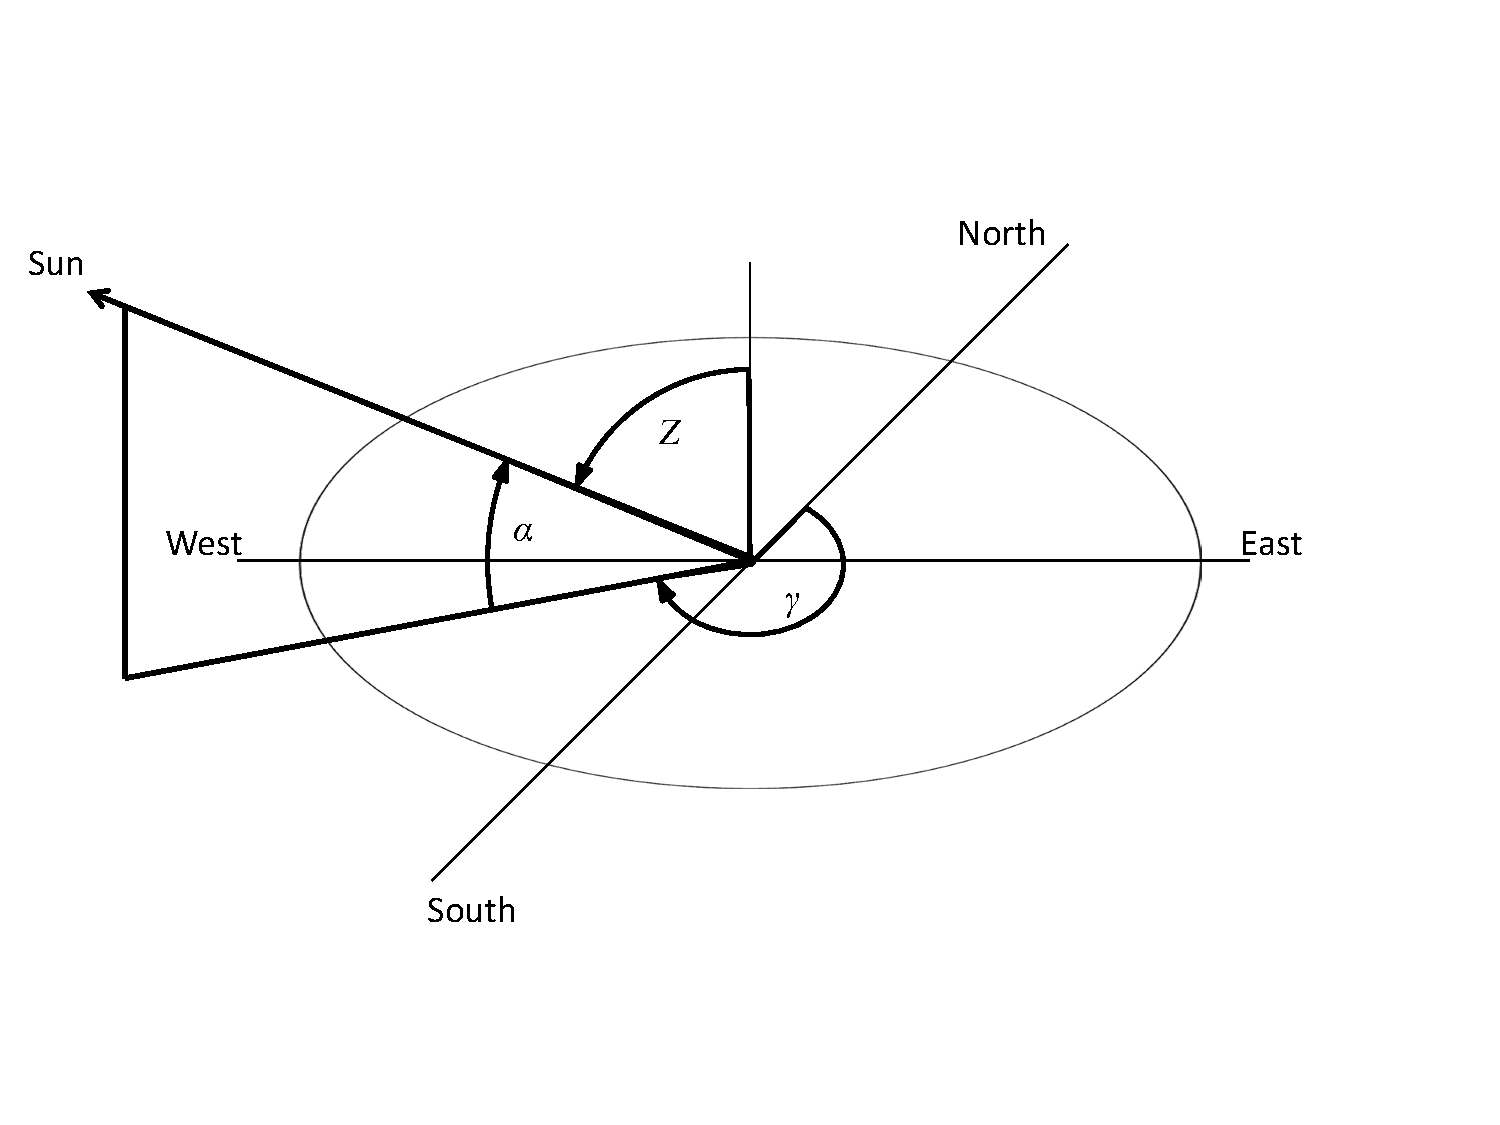
\includegraphics[scale=0.6]{sun-angles}
\caption{Sun Angles}
\label{fig-sunangles}
\end{center}
\end{figure}

\section{Effective Time}

The first step in the sun position algorithm is to determine the effective time of the current time step. SAM reads the time stamp data for the current time step in the weather file (represented by a data row) as a year, month, day, hour, and minute value. %lib_irradproc.cpp 102

The standard weather files from the National Solar Radiation Database \citep{nsrdb} start at $hr=1$. The algorithm converts the first hour number $hr=0$: 
\begin{equation}
hr=hr-1
\end{equation}

The algorithm uses the midpoint of the time step for sun position calculations (except for the hours containing sunrise and sunset, see Section~\ref{sec-sunriseset}), and assumes an hourly time step, so it replaces the minute value from the weather file: %eg, for tmy2 format see weatherfile.cpp 601
\begin{equation}\label{eqn-mn30}
\mathit{min} =30
\end{equation}

%lib_irradproc.cpp 102
The Julian day of year $\mathit{jdoy}$ is the number of days since Noon on January 1 of the current year (strictly speaking, it should be called the \textit{ordinal date}). Because some weather files are typical year files, the time stamps in a given file may not all use the same year. For example, all January time stamps may be 1988, while all February time stamps may be 2005 \citep{tmy3}.

To account for leap years:
%lib_irradproc.cpp 26
\begin{equation}
k = 
\left\{
   \begin{array}{ll}
      1 & \text{if $\mathit{year}\mod4=0$}\\
      0 & \text{if $\mathit{year}\mod4\neq0$}\\
   \end{array}
\right. 
\end{equation}

Note that this accounts for leap years to correctly calculate effective time, but is separate from the energy simulation, which does not account for leap years.

%lib_irradproc.cpp 31
SAM calculates the number of days since January 1 $a$ from the number of days in each of the months (January = 31, February = 28, March = 31, etc.) before the current month, and the number of days since the first of the current month.

The Julian day of year is then:
%lib_irradproc.cpp 36
\begin{equation}
\mathit{jdoy}= 
\left\{
   \begin{array}{ll}
      \mathit{day} + a & \text{for January and February}\\
      \mathit{day} + a + k & \text{for March through December}
   \end{array}
\right. 
\end{equation}

The current decimal time of day expressed as an offset from UTC depends on the hour and minute of the current time stamp, and the location's time zone:
%lib_irradproc.cpp 103
\begin{equation}\label{eqn-tutc}
t_{utc} = \mathit{hr} + \frac{\mathit{min}}{60} - \mathit{tz}
\end{equation}

For some combinations of time stamp and time zone, Equation~\ref{eqn-tutc} may yield a value less than zero or greater than 24 hours, in which case the following correction applies:
%lib_irradproc.cpp 104
\begin{equation}
\left\{
   \begin{array}{ll}
      t_{utc} = t_{utc} + 24, \mathit{jdoy} = \mathit{jdoy} - 1 & 
      \text{if $t_{utc}<0$}\\
      t_{utc} = t_{utc} - 24,  \mathit{jdoy} = \mathit{jdoy} + 1 & 
      \text{if $t_{utc}>24$}
   \end{array}
\right. 
\end{equation}

The Julian date $\mathit{julian}$ of the current hour is the Julian day of the preceding noon plus the number of hours since then. The Julian day is defined as the number of days since Noon on January 1, 2000:
% time irradproc.cpp 117
\begin{equation}\label{eqn-jday}
\mathit{julian} = 32916.5 + 365(\mathit{yr}-1949) + \frac{\mathit{yr}-1949}{4} + \mathit{jdoy} + \frac{t_{utc}}{24} - 51545
\end{equation}

\section{Sun Angles} \label{sec-sunangles}

The sun angle equations are from \citet{michalsky1988}. The sun angles (Figure~\ref{fig-sunangles}) are the altitude angle $\alpha$, declination angle $\delta$, and zenith angle $Z$. SAM also calculates the sun azimuth angle $\gamma$ for use in the incident irradiance calculations. The solar declination angle is not used in the incident irradiance calculations, but is required to calculate the sun azimuth angle. The bold font in Table~\ref{tab-sunposvars} indicates that SAM reports the sun zenith, altitude, and azimuth angles in the hourly results.

The first step in the sun angle calculation for a given time step is to determine the ecliptic coordinates of the location, which define the photovoltaic array's position on the earth relative to the sun. The ecliptic coordinate variables are the mean longitude, mean anomaly, ecliptic longitude, and obliquity of the ecliptic. The algorithm uses ecliptic coordinates instead of equatorial coordinates to include the effect of the earth's inclination in the sun angle calculations.

Where limits are indicated for the equations below, if the variable's value falls outside of the limits, SAM adjusts the value. For example, for a value $x$ with the limits $0\leq\mathit{x}<360\degree$, SAM divides $x$ by $360\degree$, and checks to see whether the remainder is less than zero, and if it is, adds $360\degree$ to the remainder:
%lib_irradproc 120
\begin{align}\label{eqn-eclipticlimits}
a &= \mathit{x} - 360\degree~\text{trunc} \left(\frac{x}{360\degree}\right)\notag\\
\mathit{x}&= \left\{
  \begin{array}{ll}
    a & \text{if $a\geq0$}\\
    a+360\degree & \text{if $a<0$}
  \end{array}
\right.
\end{align}

%lib_irradproc 119-145 (mnlong is not converted to radians)
Mean longitude in degrees ($0\leq\mathit{mnlong}<360\degree$). Note that the mean longitude is the only value not converted to radians:
\begin{equation}\label{eqn-mnlong}
\mathit{mnlong} = 280.46 + 0.9856474~\mathit{julian}
\end{equation}

Mean anomaly in radians ($0\leq\mathit{mnanom}<2\pi$):
\begin{equation}\label{eqn-mnanom}
\mathit{mnanom} = \frac{\pi}{180}\left(357.528 + 0.9856003~\mathit{julian}\right)
\end{equation}

Ecliptic longitude in radians ($0\leq\mathit{eclong}<2\pi$):
\begin{equation}\label{eqn-eclong}
\mathit{eclong} = \frac{\pi}{180}\left[\mathit{mnlong} + 1.915\sin \mathit{mnanom} + 0.02\sin(2\mathit{mnanom})\right]
\end{equation}

Obliquity of ecliptic in radians:
\begin{equation}\label{eqn-oblqec}
\mathit{obleq} = \frac{\pi}{180}\left(23.439 - 0.0000004~\mathit{julian}\right)
\end{equation}

The next step is to calculate the celestial coordinates, which are the right ascension and declination.

The right ascension in radians:
%lib_irradproc.cpp 137
\begin{equation}
\mathit{ra} = \left\{
\begin{array}{ll}
\arctan\left(  \frac{ \cos\mathit{\mathit{obleq}}\sin{\mathit{eclong}}}{\cos\mathit{eclong}}  \right) + \pi & \text{if $\cos\mathit{eclong}<0$}\\
\arctan\left(  \frac{ \cos\mathit{\mathit{obleq}}\sin{\mathit{eclong}}}{\cos\mathit{eclong}}  \right) + 2\pi & \text{if $\cos\mathit{obleq}\sin\mathit{eclong}<0$}\\
\end{array}
\right.
\end{equation}

The solar declination angle in radians:
\begin{equation}\label{eqn-dec}
\delta = \arcsin \left( \sin \mathit{obleq} \sin \mathit{eclong} \right)
\end{equation}

Next are the local coordinates, which require calculating the hour angle. 

The Greenwich mean siderial time in hours ($0\leq\mathit{gmst}<24$) with limits applied as shown in Equation~\ref{eqn-eclipticlimits} depends on the current time at Greenwich $t_{utc}$ from Equation~\ref{eqn-tutc}, and the Julian day from Equation~\ref{eqn-jday}:
%lib_irradproc.cpp 147
\begin{equation}
\mathit{gmst}= 6.697375 + 0.0657098242~\mathit{julian} + t_{\mathit{utc}}
\end{equation}

Local mean siderial time in hours ($0\leq\mathit{lmst}<24$):
%lib_irradproc.cpp 152
\begin{equation}
\mathit{lmst}= \mathit{gmst} + \frac{\mathit{lon}}{15}
\end{equation}

The hour angle in radians ($-\pi<\mathit{HA}<\pi$):
%lib_irradproc.cpp 158
\begin{align}
b &= 15\frac{\pi}{180}\mathit{lmst} -\mathit{ra}\notag\\
\mathit{HA}&= \left\{
  \begin{array}{ll}
  b + 2\pi & \text{if $b<-\pi$}\\
  b - 2\pi & \text{if $b>\pi$}
  \end{array}
\right.
\end{align}

The sun altitude angle in radians, not corrected for refraction:
%lib_irradproc.cpp 166
\begin{align} \label{eqn-elv}
a &= \sin\delta \sin\left(\frac{\pi}{180}\mathit{lat}\right) + \cos\delta \cos\left(\frac{\pi}{180}\mathit{lat}\right) \cos\mathit{HA}\notag\\
\alpha_0 &=\left\{
  \begin{array}{ll}
    \arcsin a & \text{if $-1 \leq a \leq 1$}\\
    \frac{\pi}{2} & \text{if $a>1$}\\
    -\frac{\pi}{2} & \text{if $a<1$}
  \end{array}
\right.
\end{align}

The sun altitude angle $\alpha$ corrected for refraction is:
% lib_irradproc 194
\begin{align}\label{eqn-elvcorr}
\alpha_{0d} &= \frac{180}{\pi}\alpha_0\notag\\
r &= \left\{
\begin{array}{ll}
\alpha_{0d} + 3.51561\left(\frac{0.1594 + 0.0196\alpha_{0d} + 0.00002\alpha_{0d}^2}{1 + 0.505\alpha_{0d} + 0.0845\alpha_{0d}^2}\right) & \text{if $\alpha_{0d}>-0.56$}\\
0.56 & \text{if $\alpha_{0d} \leq -0.56$}
\end{array}
\right.\notag\\
\alpha & = \left\{
\begin{array}{ll}
\frac{\pi}{2} & \text{if $\alpha_{0d} + r > 90$}\\
\frac{\pi}{180}\left(\alpha_{0d} + r\right) & \text{if $\alpha_{0d} + r \leq 90$}
\end{array}
\right.
\end{align}

The sun azimuth angle $\gamma$ in radians is from \citep{iqbal1983} rather than \citep{michalsky1988} because the latter is only for northern hemisphere locations:
%lib_irradproc 174
\begin{align}\label{eqn-solaraz}
a &= \frac{\sin\alpha_0 \sin\left(\frac{\pi}{180}\mathit{lat}\right) - \sin\delta}{\cos\alpha_0 \cos\left(\frac{\pi}{180}\mathit{lat}\right)}\notag\\
b &= \left\{
\begin{array}{ll}
\arccos a & \text{if $-1 \leq a \leq 1$}\\
\pi & \text{if $\cos\alpha_0=0$, or if $a < -1$}\\
0 & \text{if $a > 1$}
\end{array}
\right.\notag\\
\gamma &= \left\{
\begin{array}{ll}
b & \text{if $\mathit{HA} < -\pi$}\\
\pi - b & \text{if $-\pi \leq \mathit{HA} \leq 0$, or if $\mathit{HA} \geq \pi$}\\
\pi + b & \text{if $0 < \mathit{HA} < \pi$}
\end{array}
\right.
\end{align}

The sun zenith angle $Z$ in radians:
%lib_irradproc 228
\begin{equation}\label{eqn-zen}
Z = \frac{\pi}{2}-\alpha
\end{equation}

\section{Sunrise and Sunset Hours}\label{sec-sunriseset}

For the hours of each day that contain the time of sunrise and sunset, it is not appropriate to use the midpoint of the hour (see Equation~\ref{eqn-mn30}) to calculate that hour's solar position because the midpoint may be before sunrise or after sunset. For the sunrise hour, the solar position angle is for the minute at the midpoint between the minute of sunrise and the end of the hour. For the sunset hour, the angle is for the midpoint between the beginning of the hour and sunset.

To determine whether the current time stamp is for an hour that contains a sunrise, or is a nighttime or daytime hour, the sunrise hour angle in radians is:
%lib_irradproc.cpp 210
\begin{align}\label{eqn-sunup}
a &= -\tan \mathit{lat}\tan\delta\notag\\
\mathit{HAR} &= 
\left\{
   \begin{array}{lll}
      0 & \text{if $a\geq1$} & \text{sun is down}\\
      \pi & \text{if $a\leq-1$} & \text{sun is up}\\
      \arccos a & \text{if $-1<a<1$} & \text{sunrise hour}
   \end{array}
\right. 
\end{align}

The equation of time in hours:
%lib_irradproc.cpp 204
\begin{align}\label{eqn-eot}
a &= \frac{1}{15}\left(\mathit{mnlong} - \frac{\pi}{180}\mathit{ra}\right)\notag\\
\mathit{EOT} &= 
\left\{
   \begin{array}{ll}
     a & \text{if $-0.33 \leq a \leq 0.33$}\\
     a + 24 & \text{if $a<-0.33$}\\
     a - 24 & \text{if $a>0.33$}
   \end{array}
\right. 
\end{align}

The sunrise time in local standard decimal time:
%lib_irradproc.cpp 219
\begin{equation}
t_{sunrise} = 12 - \frac{1}{15} \frac{180}{\pi}\mathit{HAR} - \left(\frac{\lambda}{15} - \mathit{tz}\right)-\mathit{EOT}
\end{equation}

And, the sunset in local standard time: 
\begin{equation}
t_{sunrise} = 12 + \frac{1}{15} \frac{180}{\pi}\mathit{HAR} - \left(\frac{\lambda}{15} - \mathit{tz}\right)-\mathit{EOT}
\end{equation}

The solar position minute for the sunrise hour is at the midpoint between the minute during which the sun rose and the end of the current hour. Assuming a 60 minute time step and that that the sunup time is in decimal minutes: 
%adapted from irradproc.cpp 847 for 60 minute (3600 second) time step
\begin{equation}
\mathit{min}_{sunrise}=60 \left(1 - (t_{sunrise} -\mathit{hr}) + \frac{(t_{\mathrm{sunrise}} - hr)}{2}\right)
\end{equation}

Similarly, the solar position minute for the sunset hour is at the midpoint between the beginning of the current hour and the minute during which the sun set:
\begin{equation}
\mathit{min}_{\mathrm{sunset}}=\frac{60 (t_{\mathrm{sunset}} - \mathit{hr})}{2}
\end{equation}

\section{Sunup Flag}\label{sec-sunup}

The sunup flag indicates whether the sun is above or below the horizon in the current hour. It is determined from the sunrise hour angle (Equation~\ref{eqn-sunup}):
  \begin{itemize}
  \item If the sun is down in the current hour, $\mathit{sunup} = 0$.
  \item If the sun is up in the current hour, $\mathit{sunup} = 1$.
  \item If a sunrise occurs in the current hour, $\mathit{sunup} = 2$.
  \item If a sunset occurs in the current hour, $\mathit{sunup} = 3$.
  \end{itemize}


\section{Extraterrestrial Radiation}\label{sec-hextra}

Extra terrestrial radiation $H$ is the solar radiation at the top of the earth's atmosphere in $\mathrm{W/m^2}$. SAM uses the value in the incident irradiance calculations described in Section~\ref{sec-incidentirradiance}.
 
The extraterrestrial radiation equation is from Chapter 1.10 of \citet{duffie2013}:
%lib_irradproc.cpp 229
\begin{align}\label{eqn-hextra}
G_{\mathrm{on}} &= 1367 \left[1+0.033\cos\left( \frac{\pi}{180}\frac{360\mathit{doy}}{365} \right)\right]\notag\\
H &= \left\{
\begin{array}{ll}
G_{\mathrm{on}} \cos Z & \text{if $0 < Z < \frac{\pi}{2}$ (sun is up)}\\
G_{\mathrm{on}} & \text{if $Z=0$}\\
0 & \text{if $Z<0$, or if $Z>\frac{\pi}{2}$}
\end{array}
\right.
\end{align}

\section{True Solar Time and Eccentricity Correction Factor}

The sun position algorithm calculates two values that are not used by the photovoltaic performance model. 

True solar or apparent time in decimal hours:
%lib_irradproc.cpp 225
\begin{equation}
t_{\mathrm{truesolar}} = \mathit{hr} + \frac{min}{60} + \frac{\mathit{lon}}{15} - \mathit{tz} + \mathit{EOT}
\end{equation}

The eccentricity correction factor:
%lib_irradproc.cpp 222
\begin{equation}
E_0 = [ 1.00014 - 0.01671\cos\mathit{mnanom} - 0.00014\cos(2\mathit{mnanom}) ]^{-2}
\end{equation}

%%%%%%%%%%%%%%%%%%%%%%%%%%%%%%%%%%%%%%%%%%%%%%%%%%
%%%%%%%%%%%%%%%%%%%%%%%%%%%%%%%%%%%%%%%%%%%%%%%%%%
\chapter{Surface Angles}\label{sec-surfaceangles}

SAM considers each subarray in the system to be a flat surface with one tilt angle $\beta_s$ and one azimuth angle $\gamma_s$ that define the surface orientation. The surface angles depend on whether the subarray is fixed, or mounted on one-axis, two-axis, or azimuth-axis trackers. Surfaces with one-axis trackers have a third surface angle $\sigma$ defining its rotation around the tracking axis.

The surface angle equations are based on standard geometric relationships defined by the surface orientation and sun angles (Section~\ref{sec-sunangles}).

SAM calculates each subarray's surface angles for each of the 8,760 hours of the simulation. For systems with trackers, the surface angles in a given hour are fixed over the hour. Because the sun position angles are at the midpoint of the hour (except for the hours containing the sunrise and sunset (Section~\ref{sec-sunriseset}), the surface angles are also at the midpoint of the hour.

Table~\ref{tab-surfaceanglevars} defines the variables used for the equations in this section. Figure~\ref{fig-arrayorientation}, adapted from \citet{dunlap2007}, shows how the surface angles are defined.

%1205			irr.set\_sky\_model( skymodel, alb );
%				if ( radmode == 0 ) irr.set\_beam\_diffuse( wf.dn, wf.df );
%				else if (radmode == 1) irr.set\_global\_beam( wf.gh, wf.dn );

\begin{table}
\begin{center}
\caption{Surface Angle Variable Definitions}
\begin{tabular}{lll}
\midrule
Symbol & Description / \textbf{Name in SAM} & Name in SSC\\
\midrule
\multicolumn{3}{c}{Inputs}\\
- & \textbf{Fixed}, \textbf{1 Axis}, \textbf{2 Axis}, \textbf{Azimuth Axis} & \texttt{track\_mode}\\
$\beta_0$ & \textbf{Tilt (deg)}& \texttt{tilt}\\
$\gamma_0$ & \textbf{Azimuth (deg)} & \texttt{azimuth}\\
$\theta_{\mathrm{lim}}$ & \textbf{Tracker rotation limit (deg)} & \texttt{rotlim}\\
$Z$ & sun zenith angle & \texttt{sun\_zen}\\
$\gamma$ & sun azimuth angle & \texttt{sun\_azm}\\
- & \textbf{Backtracking }& \texttt{backtrack}\\
$\GCR$ & \textbf{Ground coverage ratio (GCR)} & \texttt{GCR}\\
- & \textbf{Beam and diffuse}, \textbf{Total and beam} & \texttt{irrad\_mode}\\
- & \textbf{Isotropic}, \textbf{HDKR}, \textbf{Perez} & \texttt{sky\_model}\\
\midrule
\multicolumn{3}{c}{Outputs}\\
$\AOI$ & incidence angle & \texttt{incidence}\\
$\beta_s$ & \textbf{Subarray [\textit{n}] Surface tilt (deg)} & \texttt{surf\_tilt}\\
$\gamma_s$ & \textbf{Subarray [\textit{n}] Surface azimuth (deg)} & \texttt{surf\_azm}\\
$\theta$ & \textbf{Subarray [\textit{n}] Axis rotation for 1 axis trackers (deg)} & \texttt{axis\_rotation}\\
$\theta_0$ & \textbf{Subarray [\textit{n}] Ideal axis rotation for 1 axis trackers (deg)} & -\\
$\Delta\theta$ & backtracking difference from ideal rotation & \texttt{bt\_diff}\\
\midrule
\end{tabular}
\label{tab-surfaceanglevars}
\end{center}
\end{table}

\begin{figure}
\begin{center}
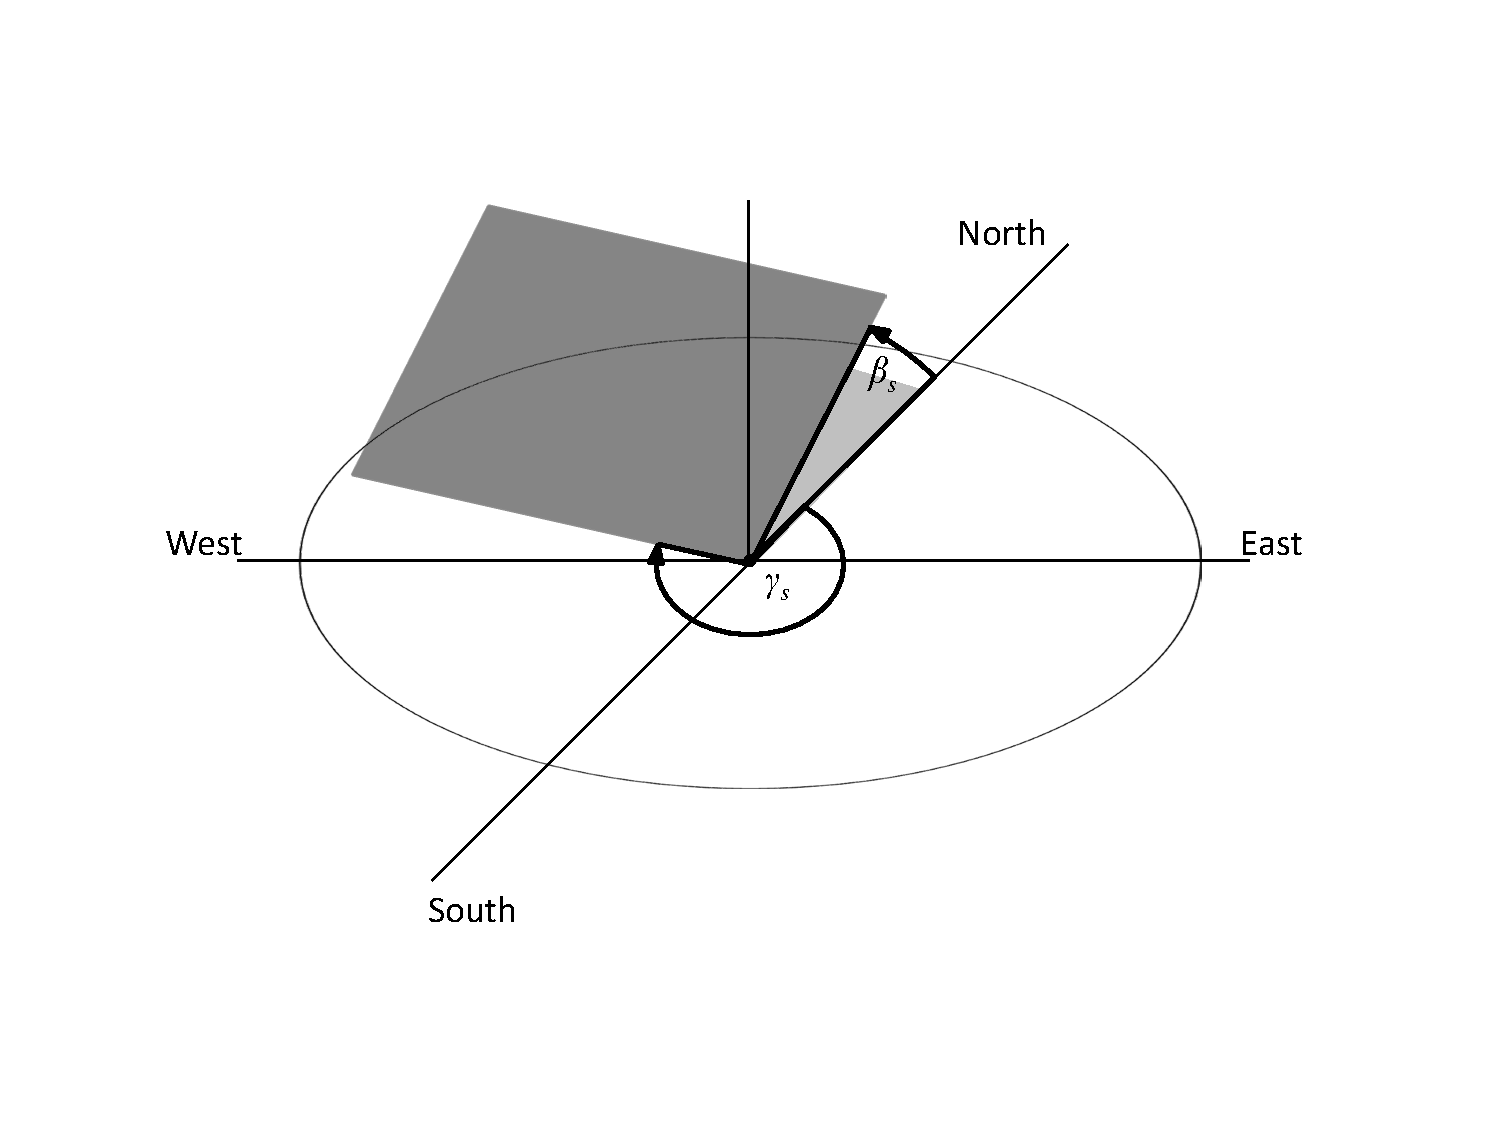
\includegraphics[scale=0.6]{surface-angles}
\caption{Surface Angles}
\label{fig-arrayorientation}
\end{center}
\end{figure}

\section{Angle of Incidence} \label{sec-theta}

The angle of incidence $\AOI$ is the sun incidence angle defined as the angle between beam irradiance and a line normal to the subarray surface (See Figure~\ref{fig-arrayorientation}). It is a function of the sun azimuth angle $\gamma$, sun zenith angle $Z$, surface azimuth angle $\gamma_s$, and the surface tilt angle $\beta_s$:
%lib_irradproc.cpp 292
\begin{align}\label{eqn-inc}
a &= \sin Z \cos(\gamma - \gamma_s) \sin\beta_s + \cos Z \cos\beta_s \notag\\
\AOI &= \left\{
\begin{array}{ll}
\pi & \text{if $a<-1$}\\
0 & \text{if $a>1$, or for two-axis tracking}\\
\arccos a & \text{if $-1 \leq a \leq 1$}
\end{array}
\right.
\end{align}

\section{Fixed, Azimuth and Two-axis Tracking}

The surface azimuth and tilt angle values depend on the tracking option as described below.

For a fixed surface (no tracking):
\begin{align}\label{eqn-fxtilt}
\beta_s &= \beta_0 \notag\\
\gamma_s &= \gamma_0
\end{align}

For azimuth tracking, the surface tilt angle is fixed, and the surface azimuth angle follows the sun azimuth angle:
\begin{align}\label{eqn-aztilt}
\beta_s &= \beta_0 \notag\\
\gamma_s &= \gamma
\end{align}

For two-axis tracking, the surface tilt and azimuth angles follow the sun zenith and azimuth angles, respectively:
\begin{align}\label{eqn-2xtilt}
\beta_s & = Z \notag\\
\gamma_s & = \gamma
\end{align}

\section{One-axis Tracking}

One-axis tracking involves a third surface angle $\theta$ describing the surface's rotation about the tracking axis and a rotation angle limit $\theta_{lim}$. 

SAM offers three shade modes for the one-axis tracking option on the PV Subarrays input page:
\begin{itemize}
\item \textbf{Self-shaded} accounts for shading of modules in one row by those in neighboring rows (see Section~\ref{sec-selfshad}), but does not model backtracking.
\item \textbf{Backtracking} adjusts the tracking angle to avoid shading of modules in one row by those in neighboring rows (see Section~\ref{sec-backtrack1x}).
\item \textbf{None} does not account for self-shading or backtracking.
\end{itemize}

All one-axis surface angle equations use angle values converted from degrees to radians.

The one-axis tracking tilt angle in radians (See Sections~\ref{sec-rot1x} and \ref{sec-backtrack1x} for rotation angle equations):
%lib_irradproc.cpp 386
\begin{align}
a & = \cos\beta_0 \cos\theta\notag\\
\beta_s &= \left\{
\begin{array}{ll}
\pi & \text{if $a<-1$}\\
0 & \text{if $a>1$}\\
\arccos a & \text{if $-1 \leq a \leq 1$}
\end{array}
\right.
\end{align}

The one-axis tracking surface azimuth angle in radians:
%lib_irradproc.cpp 394
\begin{align}
a & = \frac{\sin\theta}{\sin\beta}\notag\\
\gamma_s &= \left\{
\begin{array}{ll}
\pi & \text{if $\beta_s=0$}\\
\frac{3\pi}{2} + \gamma_0 & \text{if $a<-1$}\\
\frac{\pi}{2} + \gamma_0 & \text{if $a>1$}\\
\gamma_0 - \pi - \arcsin{a} & \text{if $\theta < -\frac{\pi}{2}$}\\
\gamma_0 + \pi - \arcsin{a} & \text{if $\theta > \frac{\pi}{2}$}\\
\gamma_0 + \arcsin{a} & \text{if $-1 \leq a \leq 1$ or $-\frac{\pi}{2} \leq \theta \leq \frac{\pi}{2}$}
\end{array}
\right.
\end{align}

The surface azimuth angle in radians must be between zero and $2\pi$:
%lib_irradproc.cpp 409
\begin{equation}
\gamma_s = \left\{
\begin{array}{ll}
\gamma_s - 2\pi & \text{if $\gamma_s > 2\pi$}\\
\gamma_s + 2\pi & \text{if $\gamma_s < 0$}
\end{array}
\right.
\end{equation}

\subsection{Rotation Angle for One-axis Trackers}\label{sec-rot1x}

For a subarray with one-axis tracking, SAM assumes that the tracker rotates about an axis tilted from the horizontal at the surface tilt angle along the line that defines the surface azimuth angle shown in Figure~\ref{fig-arrayorientation}. 

The \textbf{tracker rotation angle} $\theta$ is the angle of the subarray surface from the horizontal about the tracking axis. For a surface tilted as shown Figure~\ref{fig-arrayorientation}, the rotation angle is the angle as viewed from the raised end of the surface, with a negative rotation angle indicating counter-clockwise rotation from the horizontal. For a surface in the northern hemisphere with a surface azimuth angle of $180^\circ$, a negative rotation angle is for a surface facing east toward the morning sun with $-90^\circ$ for a vertical, east-facing surface. A positive rotation angle is for an array facing the afternoon sun, with $90^\circ$ for a vertical, west-facing surface.  In the southern hemisphere, for a surface with an azimuth angle of $0^\circ$, a negative rotation limit indicates a west-facing surface.

The \textbf{tracker rotation limit} $\theta_lim$ is the physical limit of the tracker's motion about the tracking axis in degrees with valid values between $0$ and $\pm 90^\circ$. (Note that SAM's user interface restricts the rotation limit values to $\pm 85\degree$.) For example, a tracker in the northern hemisphere with a rotation limit of 45$^\circ$ would start tracking at a rotation angle of $-45^\circ$ in the sunrise hour, and stop tracking at a rotation angle of $45^\circ$ in the sunset hour.

SAM adjusts the surface rotation angle as follows:
\begin{itemize}
\item If the tracker rotation angle exceeds the user-specified tracker rotation limit, then the tracker rotation is set to the limit.
\item If backtracking is enabled and the array is self-shaded, then the surface tilt angle is adjusted to minimize self-shading (See Section~\ref{sec-backtrack1x}).
\end{itemize}

The one-axis tracking equations described below use angle values converted from degrees to radians. SAM displays surface angle values in the results in degrees.

The ``ideal rotation angle" $\theta_0$ for one-axis tracking is the rotation angle without application of the rotation limit $\theta_{\mathrm{lim}}$ or backtracking:
%lib_irradproc.cpp 323
\begin{align}
a &= \frac{\sin Z \sin(\gamma - \gamma_s)}{\sin Z \cos(\gamma - \gamma_s) \sin\beta + \cos Z \cos\beta} \notag\\
\theta_{\mathrm{01}} &= \left\{
\begin{array}{ll}
-\frac{\pi}{2} & \text{if $a<-99,999.9$}\\
\frac{\pi}{2} & \text{if $a>99,999.9$}\\
\arctan a & \text{if $-99,999.9 \leq a \leq 99,999.9$}
\end{array}
\right.
\end{align}

The following corrections ensure that the ideal rotation angle is in the correct quadrant (II or III) when the surface azimuth angle $\gamma_s$ is less than or greater than $\pi$:
%lib_irradproc.cpp 335
\begin{equation}
\theta_0 = \left\{
\begin{array}{ll}
\theta_{\mathrm{01}} + \pi & \text{if $\gamma_s < \pi$ and $\gamma < \gamma_s \leq \gamma_s + \pi$ and $\theta_0 < 0$ (quadrant II positive rotation)} \notag\\
\theta_{\mathrm{01}} - \pi & \text{if $\gamma_s < \pi$ and $\gamma < \gamma_s \leq \gamma_s + \pi$ and $\theta_0 > 0$ (quadrant III negative rotation)} \notag\\
\theta_{\mathrm{01}} + \pi & \text{if $\gamma_s > \pi$ and $\gamma < \gamma_s \leq \gamma_s - \pi$ and $\theta_0 < 0$ (quadrant II positive rotation)} \notag\\
\theta_{\mathrm{01}} - \pi & \text{if $\gamma_s > \pi$ and $\gamma < \gamma_s \leq \gamma_s - \pi$ and $\theta_0 > 0$ (quadrant III negative rotation}
\end{array}
\right.
\end{equation}

The rotation angle in radians is the ideal rotation angle limited by the rotation limit:
%lib_irradproc.cpp 364
\begin{equation}\label{eqn-rot1x}
\theta = \left\{
\begin{array}{ll}
\theta_0 & \text{if $-\theta_{\mathrm{lim}} \leq \theta_0 \leq \theta_{\mathrm{lim}}$}\\
-\theta_{\mathrm{lim}} & \text{if $\theta_0 < -\theta_{\mathrm{lim}}$}\\
\theta_{\mathrm{lim}} &  \text{if $\theta_0 > \theta_{\mathrm{lim}}$}
\end{array}
\right.
\end{equation}

\subsection{Backtracking for One-axis Trackers}\label{sec-backtrack1x}

Backtracking is a technique used with some one-axis trackers to minimize self-shading of neighboring rows of photovoltaic modules during times that the sun is low in the sky. When neighboring rows shade each other, the tracker rotates toward the horizontal to reduce the size of shadows on the array.

SAM's backtracking for one-axis tracking algorithm was developed by NREL for SAM. It involves the following steps:
%lib_irradproc.cpp 373, 1258
\begin{enumerate}
\item Run the self-shading algorithm (Section~\ref{sec-selfshad}). It determines whether a portion of the subarray is self-shaded, given the ground coverage ratio $\GCR$, sun angles (Section~\ref{sec-sunangles}), surface angles (Section~\ref{sec-surfaceangles}), and ideal surface rotation angle $\theta_0$ (Equation~\ref{eqn-rot1x}).
\item If a portion of the subarray is self-shaded, adjust the tracker rotation angle $\theta$ toward $0^\circ$ by $1^\circ$.
\item Repeat Steps 1-2 until $F_{\mathrm{shad1x}}=0$, or one hundred times, whichever comes first (to avoid an infinite loop).
\end{enumerate}

The backtracking rotation difference $\Delta\theta$ reported by SSC as \texttt{bt\_diff}:
%lib_irradproc.cpp 379
\begin{equation}
\Delta\theta = \theta - \theta_0
\end{equation}

%%%%%%%%%%%%%%%%%%%%%%%%%%%%%%%%%%%%%%%%%%%%%%%%%%
%%%%%%%%%%%%%%%%%%%%%%%%%%%%%%%%%%%%%%%%%%%%%%%%%%
\chapter{Incident Irradiance}\label{sec-incidentirradiance}

The incident irradiance, also called plane-of-array irradiance or POA irradiance, is the solar irradiance incident on the plane of the photovoltaic array in a given time step. SAM calculates the incident irradiance for the sunrise hour, sunup hours, and sunset hour. The incident angle algorithm calculates the hourly beam and diffuse irradiance incident on the photovoltaic subarray surface for a given sun position, latitude, and surface orientation. For each  time step in the simulation, the incident irradiance algorithm steps are:

%lib_irradproc.cpp 896-938
\begin{enumerate}
\item Calculate the angle of incidence (Section~\ref{sec-theta}).
\item Calculate the beam irradiance on a horizontal surface.
\item Check to see if the beam irradiance on a horizontal surface exceeds the extraterrestrial radiation.
\item Calculate the incident beam irradiance.
\item Calculate the sky diffuse horizontal irradiance using one of the three sky diffuse irradiance methods.
\item Calculate the ground-reflected irradiance.
\end{enumerate}

\begin{table}
\begin{center}
\caption{Incident Irradiance Variable Definitions}
\begin{tabular}{lll}
\midrule
Symbol & Description / \textbf{Name in SAM} & Name in SSC\\
\midrule
\multicolumn{3}{c}{Inputs}\\
$E_b$ & \textbf{Beam irradiance}, beam normal from weather file& \texttt{beam}\\
$E_d$ & \textbf{Diffuse irradiance}, diffuse horiz. from weather file, or calculated & \texttt{diffuse}\\
$E_g$ & \textbf{Global horizontal irradiance}, global horizontal from weather file & \texttt{global}\\
$H$ & extraterrestrial irradiance  & -\\
$\mathit{\rho}$ & \textbf{Albedo} (ground reflectance)& \texttt{albedo}\\
$\AOI$ & \text{angle of incidence} & \texttt{incidence}\\
$\beta_s$ & \textbf{Subarray [\textit{n}] Surface tilt} & \texttt{tilt}\\
$Z$ & \textbf{Solar zenith angle} & \texttt{sun\_zen}\\
- & \textbf{Beam and diffuse}, \textbf{Total and beam} & \texttt{irrad\_mode}\\
- & \textbf{Isotropic}, \textbf{HDKR}, \textbf{Perez} & \texttt{sky\_model}\\
- & \textbf{Use albedo in weather file if it is specified} & \texttt{use\_wf\_albedo}\\
\midrule
\multicolumn{3}{c}{Outputs}\\
$I_b$ & incident beam irradiance & \texttt{poa\_beam}\\
$I_d$ & incident sky diffuse irradiance & \texttt{poa\_skydiff}\\
$I_r$ & incident ground-reflected irradiance & \texttt{poa\_gnddiff}\\
$D_i$ & isotropic component of incident diffuse irradiance & \texttt{poa\_skydiff\_iso}\\
$D_c$ & circumsolar component of incident diffuse irradiance & \texttt{poa\_skydiff\_cir}\\
$D_h$ & horizon brightening component of incident diffuse irradiance & \texttt{poa\_skydiff\_hor}\\
\midrule
\end{tabular}
\label{tab-incidentirradiancevars}
\end{center}
\end{table}

\section{Incident Beam Irradiance}\label{sec-incidentbeam}

The incident beam irradiance is solar energy that reaches the surface in a straight line from the sun:
%lib_irradproc.cpp 520 (isotropic), 602 (perez), 481 (hdkr)
\begin{equation}
I_b = E_b\cos\AOI
\end{equation}

The beam irradiance on a horizontal surface:
%lib_irradproc.cpp 905
\begin{equation}\label{eqn-hbeam}
I_{\mathrm{bh}}=E_b\cos Z
\end{equation}

%cmod_pvsamv1.cpp 1213
SAM compares $I_{\mathrm{bh}}$ to the extraterrestrial radiation $H$ (Equation~\ref{eqn-hextra}). If $I_{\mathrm{bh}}>H$, it generates an error flag that causes the calculations to stop and SAM to display the error message``failed to compute irradiation on surface."

\section{Incident Sky Diffuse Irradiance}

Incident sky diffuse irradiance $I_d$ is solar energy that has been scattered by molecules and particles in the earth's atmosphere before reaching the surface of the subarray.

The sky diffuse model calculates values of the components of the sky diffuse irradiance (isotropic, circumsolar, and horizon brightening), but those components are not used by the photovoltaic model. The equations are provided in the sections below for reference.%???

The \textbf{Tilted Surface Radiation Model} option on the Location and Resource input page in SAM (\texttt{sky\_model} in SSC) allows you to choose from three different sky diffuse irradiance models:

\begin{itemize}
\item The \textbf{Isotropic} model is the simplest of the three models, and assumes that diffuse radiation is uniformly distributed across the sky, called isotropic diffuse radiation ($\mathtt{sky\_model} = 0$).
\item \textbf{HDKR}, named for the algorithm developed by Hay, Davies, Klucher and Reindl in 1979, also assumes isotropic diffuse radiation, but accounts for the higher intensity of circumsolar diffuse radiation, which is the diffuse radiation in the area around the sun ($\mathtt{sky\_model} = 1$).
\item The \textbf{Perez} model uses a more complex computational method than the other two methods that accounts for both isotropic and circumsolar diffuse radiation, as well as horizon brightening ($\mathtt{sky\_model} = 2$). 
\end{itemize}

The \textbf{Radiation Components} option on the Location and Resource input page (\texttt{irrad\_mode} in SSC) allows you to choose whether to use the diffuse horizontal irradiance from the weather file, or whether to calculate it from the global horizontal and beam normal irradiance values:
%lib_irradproc.cpp 914
\begin{equation}\label{eqn-diffhoriz}
E_d = \left\{
\begin{array}{ll}
E_d & \text{Use weather file value if option is \textbf{Beam and diffuse} ($\texttt{irrad\_mode}=0)$}\\
E_g - E_b\cos Z & \text{Calculate for \textbf{Total and beam} ($\texttt{irrad\_mode}=1)$}
\end{array}
\right.
\end{equation}

\subsection{Isotropic Model}

The isotropic diffuse sky irradiance \citep{liu1963}:
%lib_irradproc 521
\begin{equation}
I_d = E_d\frac{1 + \cos\beta}{2}
\end{equation}

The isotropic model does not account for circumsolar diffuse irradiance or horizon brightening:
\begin{align}
D_i &= I_d \notag\\
D_c &= 0 \notag\\
D_h &= 0
\end{align}

\subsection{HDKR Model}

The Hay, Davies, Klucher, Reindl (HDKR) sky diffuse model is from Chapter 2.16 of \citet{duffie2013} and \citet{reindl1988}.

The total irradiance incident on a horizontal surface:
%lib_irradproc.cpp 465
\begin{equation}
I_{\mathrm{gh}} = I_{\mathrm{bh}} + E_d
\end{equation}

The ratio of incident beam to horizontal beam:
%lib_irradproc.cpp 469
\begin{equation}
R_b = \frac{\cos\AOI}{\cos Z}
\end{equation}

The anisotropy index for forward scattering circumsolar diffuse irradiance depends on the beam horizontal irradiance $I_{\mathrm{bh}}$ and extraterrestrial irradiance $H$ (Equation~\ref{eqn-hextra}):
%lib_irradproc.cpp 470
\begin{equation}
A_i = \frac{I_{\mathrm{bh}}}{H}
\end{equation}

The modulating factor for horizontal brightening correction:
%lib_irradproc.cpp 471
\begin{equation}
f =\sqrt{\frac{I_{\mathrm{bh}}}{I_{\mathrm{gh}}}}
\end{equation}

The horizon brightening correction factor:
%lib_irradproc.cpp 472
\begin{equation}
s =\sin^3\frac{\beta_s}{2}
\end{equation}

The circumsolar, isotropic, and horizon brightening components of the diffuse sky radiation are then:
%lib_irradproc.cpp 477
\begin{align}
\mathit{cir} &= E_d A_i R_b \notag\\
\mathit{iso} &= E_d \left( 1 - A_i \right) \frac{1 + \cos\AOI}{2} \notag\\
\mathit{isohor} &= \mathit{iso} \left( 1 + f s \right)
\end{align}

The isotropic, circumsolar, and horizon brightening components of the incident diffuse irradiance:
\begin{align}
D_i &= \mathit{iso} \notag\\
D_c &= \mathit{cir} \notag\\
D_h &= \mathit{isohor} - \mathit{iso}
\end{align}

The HDKR sky diffuse irradiance:
%lib_irradproc.cpp 482
\begin{equation}
I_d = \mathit{isohor} + \mathit{cir}
\end{equation}

\subsection{Perez 1990 Model}\label{sec-perez}

SAM's Perez sky diffuse irradiance model was adapted from PVWatts Version 1 \citep{dobos2013a} and is described in \citet{perez1988} and \citep{perez1990}. The SAM (and PVWatts) implementation includes a modification of the Perez model that treats diffuse radiation as isotropic for $87.5\degree \leq Z \leq 90\degree$. See also \citep{pvmcperez} for a general description of the model.

The Perez model differs from the isotropic and HDKR models in that it uses the empirical  coefficients in Table~\ref{tab-perezcoeffs} derived from measurements over a range of sky conditions and locations instead of mathematical representations of the sky diffuse components.

The parameters $a$ and $b$ describe the view of the sky from the perspective of the surface:
%lib_irradproc.cpp 622 656
\begin{align}
a &= \max( 0, \cos\AOI ) \notag\\
b & =\max( \cos85\degree, \cos\AOI) 
\end{align}

The sky clearness $\epsilon$ with $\kappa=5.534\times10^{-6}$ and the sun zenith angle
 $Z$ in degrees:
%lib_irradproc.cpp 584 647
\begin{equation}\label{eqn-perezepsilon}
\epsilon =\frac{(E_d + E_b ) / E_d + \kappa Z^{3} }{1 +  \kappa Z^{3}}
\end{equation}

The absolute optical air mass with the incidence angle $b$ and sun zenith angle $Z$ in degrees:
%lib_irradproc.cpp 644
\begin{equation}\label{eqn-perezam}
\mathit{AM}_0 = \left[ \cos b + 0.15~( 93.9\degree - Z )^{-1.253} \right]^{-1}
\end{equation}

The sky clearness $\Delta$ assumes an extraterrestrial irradiance value of $1,367.0~\mathrm{W/m^2}$:
%lib_irradproc.cpp 645
\begin{equation}
\Delta = E_d \frac{\mathit{AM}_0}{1367}
\end{equation}

The coefficients $F_1$ and $F_2$ are empirical functions of the sky clearness $\epsilon$ and describe circumsolar and horizon brightness, respectively. The sun zenith angle $Z$ is in radians:
%lib_irradproc.cpp 653
\begin{align}\label{eqn-perezF1F2}
F_1 & = \max \left[ 0,  \left( f_{\mathrm{11}}(\epsilon) + \Delta f_{\mathrm{12}}(\epsilon) + Z f_{\mathrm{13}}(\epsilon) \right) \right ] \notag\\
F_2 &= f_{\mathrm{21}}(\epsilon) + \Delta f_{\mathrm{22}}(\epsilon) + Z f_{\mathrm{23}}(\epsilon)
\end{align}

SAM uses a lookup table with empirical values shown in Table~\ref{tab-perezcoeffs} to determine the value of the $f$ coefficients in Equation~\ref{eqn-perezF1F2} for a given sky clearness coefficient $\epsilon$ from Equation~\ref{eqn-perezepsilon}.

%lib_irradproc.cpp 570
\begin{table}
\begin{center}
\caption{Perez Sky Diffuse Irradiance Model Coefficients}
\begin{tabular}{l|...|...}
\hline
\multicolumn{1}{c|}{} & 
\multicolumn{1}{c}{$f_{\mathrm{11}}$}  & 
\multicolumn{1}{c}{$f_{\mathrm{12}}$} & 
\multicolumn{1}{c|}{$f_{\mathrm{13}}$} & 
\multicolumn{1}{c}{$f_{\mathrm{21}}$} & 
\multicolumn{1}{c}{$f_{\mathrm{22}}$} & 
\multicolumn{1}{c}{$f_{\mathrm{23}}$} \\
\hline
$\epsilon \leq 1.065$ & -0.0083117 & 0.5877285 & -0.0620636 & -0.0596012 & 0.0721249 & -0.0220216\\
$\epsilon \leq 1.23$ & 0.1299457 & 0.6825954 & -0.1513752 & -0.0189325 & 0.065965 & -0.0288748 \\
$\epsilon \leq 1.5$  & 0.3296958 & 0.4868735 & -0.2210958 & 0.055414 & -0.0639588 & -0.0260542 \\
$\epsilon \leq 1.95$ & 0.5682053 & 0.1874525 & -0.295129 & 0.1088631 & -0.1519229 & -0.0139754 \\
$\epsilon \leq 2.8$ & 0.873028 & -0.3920403 & -0.3616149 & 0.2255647 & -0.4620442 & 0.0012448 \\
$\epsilon \leq 4.5$  & 1.1326077 & -1.2367284 & -0.4118494 & 0.2877813 & -0.8230357 & 0.0558651 \\
$\epsilon \leq 6.2$ & 1.0601591 & -1.5999137 & -0.3589221 & 0.2642124 & -1.127234 & 0.1310694 \\
$\epsilon > 6.2$ & 0.677747 & -0.3272588 & -0.2504286 & 0.1561313 & -1.3765031 & 0.2506212 \\
\hline
\end{tabular}
\label{tab-perezcoeffs}
\end{center}
\end{table}

The isotropic, circumsolar, and horizon brightening components of the sky diffuse irradiance:
\begin{equation}
\begin{array}{ll}
D_i = E_d (1-F_1) \frac{1+\cos\beta}{2} & \text{if $0\degree \leq Z \leq 87.5\degree$} \notag\\
D_c = E_d F_1 \frac{a}{b}&\notag\\
D_h = E_d F_2 \sin\beta &
\end{array}
\begin{array}{ll}
D_i =\frac{1+\cos\beta}{2} & \text{if $87.5\degree < Z < 90\degree$}~~\text{(isotropic only)} \notag\\
D_c = 0 &\\
D_h = 0 &
\end{array}
\end{equation}

The Perez incident diffuse irradiance:
\begin{equation}
I_d = D_i + D_c + D_h
\end{equation}

\section{Incident Ground-reflected Irradiance}

The incident ground-reflected irradiance is solar energy that reaches the array surface after reflecting from the ground. The ground reflects light diffusely, so the ground-reflected irradiance is diffuse irradiance. It is a function of the beam normal irradiance and sun zenith angle, sky diffuse irradiance, and ground reflectance (albedo) \citep{liu1963}:
%lib_irradproc.cpp 522
\begin{equation}
I_{r}= \mathit{\rho} \left( E_b \cos Z + E_d \right) \frac{( 1 - \cos\beta )}{2}
\end{equation}

The albedo is either the set of twelve user-specified values from the Location and Resource input page, or the value from the weather file, depending on whether the option on the Location and Resource input page \textbf{Use albedo in weather file if it is specified} is checked ($\texttt{use\_wf\_albedo=1}$ in SSC) and there is albedo data in the weather file. NSRDB TMY3 weather files typically include albedo values, while the other formats do not. Otherwise ($\texttt{use\_wf\_albedo=1}$ in SSC), SAM uses the twelve monthly albedo values from the Location and Resource input page ($\texttt{albedo}$ in SSC), assuming that the albedo is constant over a single month.

%%%%%%%%%%%%%%%%%%%%%%%%%%%%%%%%%%%%%%%%%%%%%%%%%%
%%%%%%%%%%%%%%%%%%%%%%%%%%%%%%%%%%%%%%%%%%%%%%%%%%
\chapter{Effective POA Irradiance}\label{sec-effectiveirradiance}

The effective, or plane-of-array (POA) irradiance is the incident irradiance less losses due to near-object shading, self shading, and soiling. A set of user-specified adjustment factors represents near-object shading and soiling, and must be generated outside of SAM, either by separate computer models, or by measuring equipment and its associated software. SAM calculates the self-shading factors (Section~\ref{sec-selfshad}) for fixed arrays and for subarrays with one-axis tracking.

\begin{table}
\begin{center}
\caption{Effective POA Irradiance Variable Definitions}
\begin{tabular}{lll}
\midrule
Symbol & Description / \textbf{Name in SAM} & Name in SSC\\
\midrule
\multicolumn{3}{c}{Inputs}\\
$I_b$ & incident beam irradiance  & \texttt{poa\_beam}\\
$I_d$ & incident sky diffuse irradiance & \texttt{poa\_skydiff}\\
$I_r$ & incident ground-reflected irradiance & \texttt{poa\_gnddiff}\\
$L_h$ & 8,760 hourly beam shading loss percentages  & \texttt{poa\_beam}\\
$L_{mh}$ & hour-by-month beam shading loss percentages & \texttt{subarray[\textit{n}]\_shading\_mxh}\\
$L_{azal}$ & sun azimuth-by-altitude beam shading loss percentages & \texttt{subarray[\textit{n}]\_shading\_azal}\\
$L_{dns}$ & near object sky diffuse shading loss percentage  & \texttt{subarray[\textit{n}]\_shading\_diff}\\
$L_{soilng}$ & monthly soiling loss percentages  & \texttt{subarray[\textit{n}]\_soiling}\\
\midrule
\multicolumn{3}{c}{Outputs}\\
$I$ & \textbf{...Nominal POA total irradiance} & \texttt{...poa\_nom}\\
$G_{g,shad}$ & \textbf{...POA total irradiance after shading only} & \texttt{...poa\_shaded}\\
$G_b$ & \textbf{...POA beam irradiance after shading and soiling} & \texttt{...poa\_eff\_beam}\\
$G_d$ & \textbf{...POA diffuse irradiance after shading and soiling} & \texttt{...poa\_eff\_skydiff}\\
$G$ & \textbf{...POA total irradiance after shading and soiling} & \texttt{...poa\_eff}\\
$S_{bns}$ & \textbf{...Beam irradiance shading factor} & \texttt{...beam\_shading\_factor}\\
$O$ & \textbf{...Soiling loss} & \texttt{...soiling\_derate}\\
\midrule
\multicolumn{3}{l}{Ellipses (...) indicate \textbf{Subarray [\textit{n}]} in SAM, and \texttt{hourly\_subarray[\textit{n}]\_} in SSC}\\
\multicolumn{3}{l}{For self-shading variable definitions, see Section~\ref{sec-selfshad}}\\
\end{tabular}
\label{tab-effectiveirradiancevars}
\end{center}
\end{table}

The effective irradiance is the solar energy that reaches the top of the module cover. The module submodel (Section~\ref{sec-module}) accounts for the effect of the module cover on the energy that reaches the photovoltaic cell including angle-of-incidence and reflection losses. Each module submodel option uses a different approach to calculating these losses.

\section{Nominal Global Incident Irradiance}\label{sec-nominalincidentirradiance}

The nominal global incident irradiance $I$ in $\mathrm{kW/m^2}$ is the sum of the incident beam irradiance, incident sky diffuse irradiance, and incident ground-reflected irradiance:
%cmod_pvsamv1.cpp 1226
\begin{equation}
I = I_{b} + I_{d} + I_{r}
\end{equation}

\section{Near Object Shading}\label{sec-nearobjectshad}

%pvsamv1.cpp  1240
Near-object shading is a reduction in the POA incident irradiance by objects near the array, such as buildings, poles, trees, hills, etc. Near-object shading reduces both the beam and diffuse POA irradiance.

SAM represents the reduction in beam POA irradiance using a set of beam shading losses. A beam shading loss is a percentage that represents a reduction in the POA beam irradiance for a given hour. A shading loss of zero represents no shading. A shading loss of 100\% represents complete shading.

SAM stores a set of shading losses for each subarray. The losses are specified in the Edit Shading Data window, which opens from the Shading input page when you click the \textbf{Edit Shading} button for a subarray.

SAM reads beam shading losses from three different lookup tables that make it possible to use shading data from different sources, such as shade analysis tools and modeling software:
\begin{itemize} 
\item \textbf{Hourly} is a column of 8,760 shading losses, one for each hour of the year.
\item \textbf{Hour by month} is a 24-by-12 table of 288 shading losses with one value for each hour of the day by month. For each month, SAM applies the same shading loss to a given hour of the day.
\item \textbf{Solar azimuth by altitude} is a table of shading losses for a range of sun azimuth and altitude angles. SAM uses bilinear interpolation to calculate the shading loss for a given hour based on that hour's solar position angles and four shading losses from the table.
\end{itemize}

SAM's user interface provides access to conversion functions that allow for importing shading data from files created by either the PVsyst, Solmetric SunEye, or SolarPathfinder\texttrademark~software as described in \citet{help-shading}. The conversion functions translate the data from the files into the appropriate table listed above. These functions are not available in SSC.

The shading loss inputs are expressed as percentages. SAM converts each percentage to a factor using the equation:
\begin{equation}
S=1-\frac{L}{100\%}
\end{equation}

The beam near-object shading factor for a given hour is the product of the values in the three beam shading loss factors:
%pvsamv1.cpp 1235
\begin{equation}\label{eqn-sbns}
S_{bns}=S_{hr}~S_{mh}~S_{azalt}
\end{equation}

The sky diffuse near-object shading factor $S_{dns}$ is a single value that represents a reduction in the POA diffuse irradiance for the entire year.

\subsection{3D Shade Calculator}\label{sec-3dshad}

**ARON, STEVE**

The 3D shade calculator calculates a set of beam and diffuse shade factors from a three-dimensional representation of the photovoltaic array and nearby shading objects.

\subsection{Import Shade Data}\label{sec-importshad}

**JANINE** (per Aron SAM meeting 10/14 -- maybe for Help instead? Should we document here if not part of SSC?)

\section{Snow Coverage}\label{sec-snow}

**SEVERIN**

The snow coverage model uses snow depth data in the weather file to estimate the portion of the array that is covered by snow and calculate a reduction in incident irradiance.

\section{Self Shading}\label{sec-selfshad}

Self shading is shading of photovoltaic modules in one row by modules in a neighboring rows. SAM uses the same self-shading model for fixed subarrays (no tracking) and subarrays with one-axis tracking. SAM does not model self shading for subarrays with two-axis or azimuth-axis tracking. Because the model assumes that modules consist of photovoltaic cells with three bypass diodes, it is suitable for modules mono- or poly-crystalline silicon photovoltaic cells, but not for thin film modules.The self-shading algorithm is described in detail in Section~\ref{sec-selfshadalg}.

The self-shading algorithm calculates three factors:
\begin{itemize}
\item Sky diffuse shading factor $F_{dss}$ that reduces the POA incident diffuse irradiance
\item Ground-reflected diffuse shading factor $F_{gss}$ that also reduces the POA incident diffuse irradiance
\item Beam DC loss factor $F_{dcss}$ that applies to the DC output of the array
\end{itemize}

\section{Effective Irradiance after Shading Only}

SAM reports the effective irradiance after shading only (and before soiling) for reference. It is an intermediate value that is not used in any calculations.

The beam, sky diffuse, and ground-reflected components of the effective irradiance after shading only are:
\begin{align}
G_{bshad} &= I_b~S_{bns}\notag\\
G_{dshad} &= I_d~S_{dns}~S_{dss} & S_{dss}&=1 ~\text{if no self shading} \notag\\
G_{rshad} &= I_r~S_{rss} & S_{rss}&=1 ~\text{if no self shading}
\end{align}

The global effective irradiance after shading only:
\begin{equation}
G_{shad} = G_{bshad} + G_{dshad} + G_{rshad}
\end{equation}

\section{Soiling}\label{sec-soiling}

Soiling losses are caused by a reduction in the incident irradiance due to dust and dirt on the module surface. SAM accounts for soiling losses using a set of monthly soiling loss percentages that are user inputs on the Losses input page (\texttt{subarray[\textit{n}]\_soiling} in SSC). The soiling loss applies to both the beam and diffuse components of the incident irradiance.

SAM converts each soiling loss percentage to a factor:
\begin{equation}
O=1-\frac{L}{100\%}
\end{equation}

For each hour of each month, SAM applies that month's soiling factor $O$ to all components of the incident irradiance.

\section{Effective Irradiance after Shading and Soiling}

The effective irradiance after shading and soiling is the irradiance value that the module models use as input (see Section~\ref{sec-module}).

The components of the effective irradiance after shading and soiling are, where $O$ is the soiling factor:
\begin{align} \label{eqn-effectivebeamdiffuse}
G_b &= G_{bshad}~O \notag\\
G_d &= G_{dshad}~O\notag\\
G_r &=  G_{rshad}~O
\end{align}

SAM reports the global effective irradiance $G$ and the total diffuse effective irradiance $G_{d,t}$ in the hourly results. (Note that the module submodels use the component values in Equation~\ref{eqn-effectivebeamdiffuse} as input rather than the global value.):
\begin{align}
G &= G_b + G_d + G_r\notag\\
G_{d,t} & = G_d + G_r
\end{align}

SAM also reports the effective beam shading factor $S_b$ in the hourly results ($S_{bns}$) is the near-object shading factor from Equation~\ref{eqn-sbns}:
%cmod_pvsamv1.cpp 1336
\begin{equation}
S_b = \left\{
\begin{array}{ll}
S_{bns}~S_{ss}~O &\text{for fixed self shading}\\
S_{bns}~O &\text{for one-axis self shading} 
\end{array}
\right.
\end{equation}

%%%%%%%%%%%%%%%%%%%%%%%%%%%%%%%%%%%%%%%%%%%%%%%%%%
%%%%%%%%%%%%%%%%%%%%%%%%%%%%%%%%%%%%%%%%%%%%%%%%%%
\chapter{Self Shading Algorithm}\label{sec-selfshadalg}

%cmod_pvsamv1.cpp 1039: sscalc is a class of type selfshade_t, which is defined
%in lib_pvshade.h 81 and implemented in lib_pvshade.cpp 153.
This section describes SAM's self-shading model \citep{deline2013a}. It supplements Section~\ref{sec-selfshad} and is presented here for clarity because of the length of the algorithm.

To model self shading for a subarray with no tracking (fixed) or one-axis tracking in SAM, after specifying the tracking and orientation options on the System Design page, on the Shading page, for the subarray's \textbf{Shading mode} input, choose \textbf{self-shaded}. (For a description of the backtracking algorithm for one-axis tracking, see Section~\ref{sec-backtrack1x}.) In SSC, to enable self shading, set the \texttt{pvsamv1} input variable \texttt{subarray[n]\_shade\_mode} to zero.

%self shading inputs ssinputs pvsamv1 update 76.
\begin{table}
\begin{center}
\caption{Self Shading Variable Definitions}
\begin{tabular}{lll}
\midrule
Symbol & Description / \textbf{Name in SAM} & Name in SSC\\
\midrule
\multicolumn{3}{c}{Inputs}\\
$M_{total}$ & \textbf{Modules in subarray} & -\\
$M_{string}$ & Number of modules per string & -\\
$M_{side}$ & \textbf{Number of modules along side of row} & \texttt{subarray[\textit{n}]\_nmody}\\
$M_{bottom}$ & \textbf{Number of modules along bottom of row} & \texttt{subarray[\textit{n}]\_nmodx}\\
$N_{strings}$ & Number of strings in parallel & \texttt{strings\_in\_parallel}\\
$\GCR$ & \textbf{GCR}, ground coverage ratio & \texttt{subarray[\textit{n}]\_gcr}\\
$A_m$ & module area & \texttt{[spe,cec,6par,snl]\_area}\\
$\beta_s$ & surface tilt angle & \texttt{subarray[\textit{n}]\_tilt} \\
$\gamma_s$ & surface azimuth angle & \texttt{subarray[\textit{n}]\_azimuth} \\
$Z$ & sun zenith angle & -\\
$\gamma$ & sun azimuth angle & - \\
$E_b$ & direct normal irradiance (from weather file) & - \\
$G_b$ & POA beam irradiance & - \\
$G_d$ & POA diffuse irradiance (sky and ground) & - \\
$\rho$ & albedo (from weather file, or set to 0.2) & \texttt{albedo} \\
\midrule
\multicolumn{3}{c}{Outputs}\\
$S_{dss}$ & sky diffuse factor  / \textbf{Self-shading diffuse derate}& \texttt{hourly\_ss\_diffuse\_derate}\\
$S_{rss}$ & ground diffuse factor  / \textbf{Self-shading reflected derate}& \texttt{hourly\_ss\_reflected\_derate}\\
$F_{dcss}$& DC loss factor / \textbf{Self-shading derate} & \texttt{hourly\_ss\_derate}\\
\end{tabular}
\label{tab-selfshadinputs}
\end{center}
\end{table}

The self-shading model consists of two sets of equations, one to calculate the reduction in diffuse POA irradiance, and a separate one to calculate a DC loss factor to account for the non-linear performance impact of the beam POA irradiance reduction:

\begin{itemize}
\item Reduction in diffuse POA irradiance:
\begin{enumerate}
\item Calculate the shade mask angle $\psi$ and ground coverage ratio $\GCR$.
\item Calculate the reduction in sky diffuse radiation.
\item Calculate the reduction in ground-reflected diffuse radiation.
\end{enumerate}
\item Reduction in beam POA irradiance:
\begin{enumerate}
\item Calculate the shadow dimensions $X$ and $S$.
\item Calculate the fixed self-shading DC loss factor to account for the beam POA reduction's impact on the array's output.
\end{enumerate}
\end{itemize}

Some diffuse radiation is always blocked by neighboring rows of modules, regardless of whether the rows block beam radiation \citep{goswami1989}. The diffuse radiation consists of a sky diffuse component and a ground-reflected component, both of which are affected in this way.

Table~\ref{tab-selfshadinputs} and Figure~\ref{fig-selfshaddimensions} show the variables used to calculate the fixed self-shading factors. The equations and algorithm are described in \citep{appelbaum1979} and \citep{deline2013a}.
%lib_pvshade.cpp 153 selfshade_t::init, also see cmod_pvsamv1.cpp 250 and 1047

\begin{figure}
\begin{center}
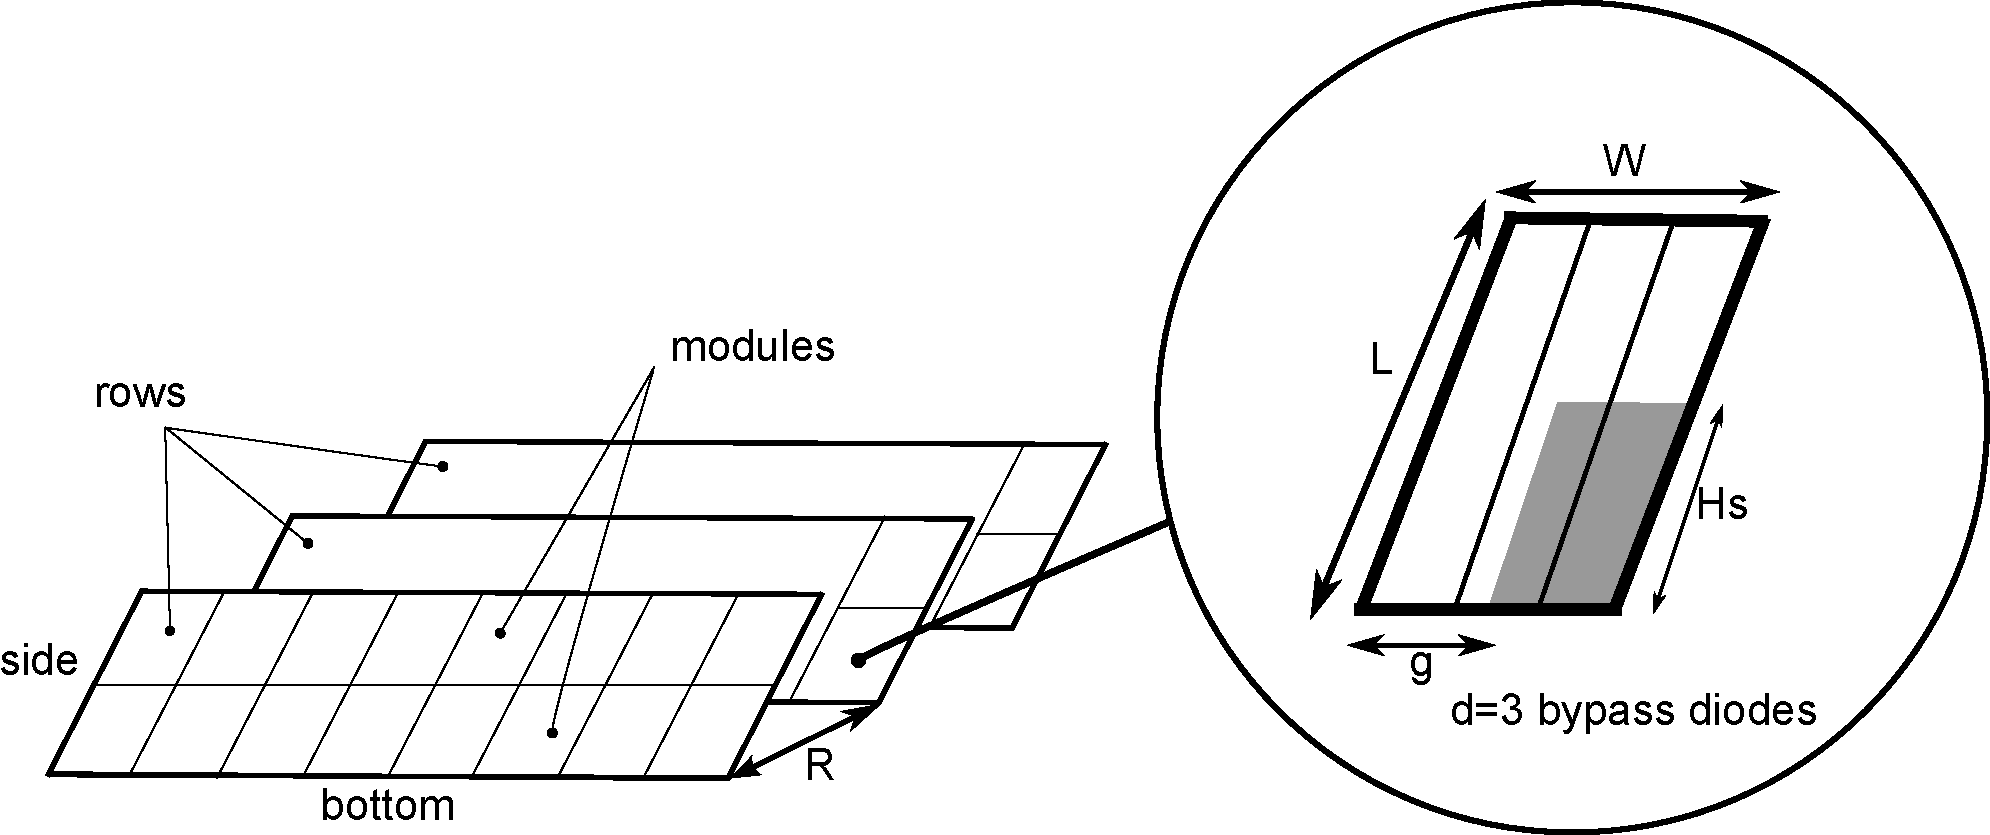
\includegraphics[scale=0.33]{self-shading-shadow-dimensions}
\caption{Shadow Dimensions for Portrait Module Orientation}
\label{fig-selfshaddimensions}
\end{center}
\end{figure}

%%%%%%%%%%%%%%%%%%%%%%%%%%%%%%%%%%%%%%%%%%%%%%%%%%
\section{Self Shading Assumptions}\label{sec-selfshadgeom}

The self-shading model makes a set of simplifying assumptions to minimize the number of inputs:

\begin{itemize}
\item Modules have an aspect ratio of $R_{aspect}=1.7$, so that the length of the long side is 1.7 times the length of the short side. 
\item The module area $A$ is the product of the module's total length and width. The value may be from one of the module libraries or a user input.
\item Each module has three bypass diodes $d=3$ so that the module is made up of three ``submodules." A submodule is a string of photovoltaic cells in the module protected by a single bypass diode. For example, a 60-cell module would consist of three submodules of 20 cells each. This assumption makes the algorithm unsuitable for modeling self shading of thin film modules.
\item A partially shaded submodule behaves in the same way as it would if the entire submodule were uniformly shaded.
\item Modules are wired together in strings parallel to the ground (horizontal strings) so that the number of modules along the bottom of a subarray row is a multiple of the number of modules per string.
\item Parallel strings in the subarray are uniformly shaded.
\end{itemize}

Based on the simplifying assumptions listed above, the number of rows $N_{rows}$ in a subarray is:
%pvsamv1 update 767
\begin{equation}
N_{rows} = \left\lfloor \frac{M_{total}}{M_{side} M_{bottom}} \right\rfloor
\end{equation}
where $M_{total}$ is the number of modules in the subarray $M_{total}=M_{string}N_{strings}$. Note that if $M_{total}$ is not an even multiple of the product $M_{string}N_{strings}$, SAM generates a simulation message indicating that the self-shading configuration does not match the subarray configuration, but still calculates the DC loss factor as described below.

SAM calculates the module length and width from the module area $A$ in $\text{m}^2$  and the fixed aspect ratio assumption  $R_{aspect}=1.7$:
%pvsamv1 update 1111
\begin{align}
W &= \sqrt{ \frac{A_m}{R_{aspect}}}\\
L &= W \mathit{R_{aspect}}
\end{align}

The module area is either from the module library, or an input, depending on the module submodel (see Section~\ref{sec-moduleoptions}).

The length of the side of a row (distance from the bottom edge to the top edge of a row):
%pvsamv1 update 1119
%this is Deline B = Applebaum A
\[
B=
  \left\{
    \begin{array}{ll}
      M_{side} L & \mbox{portrait module orientation}\\
      M_{side} W & \mbox{landscape module orientation}
    \end{array}
  \right.
\]

The distance between bottom edges of neighboring rows:
%pvsamv1 update 1123
\begin{equation}
R = \frac{B}{\GCR} 
\end{equation}
where $\GCR$ is the ground coverage ratio.

The sun altitude angle:
\begin{equation}
\alpha = 90^\circ-Z
\end{equation}

%%%%%%%%%%%%%%%%%%%%%%%%%%%%%%%%%%%%%%%%%%%%%%%%%%
\section{Shade Mask Angle}

The equations for the reduction in sky diffuse irradiance require values for the shade mask angle and ground coverage ratio.

\begin{figure}
\begin{center}
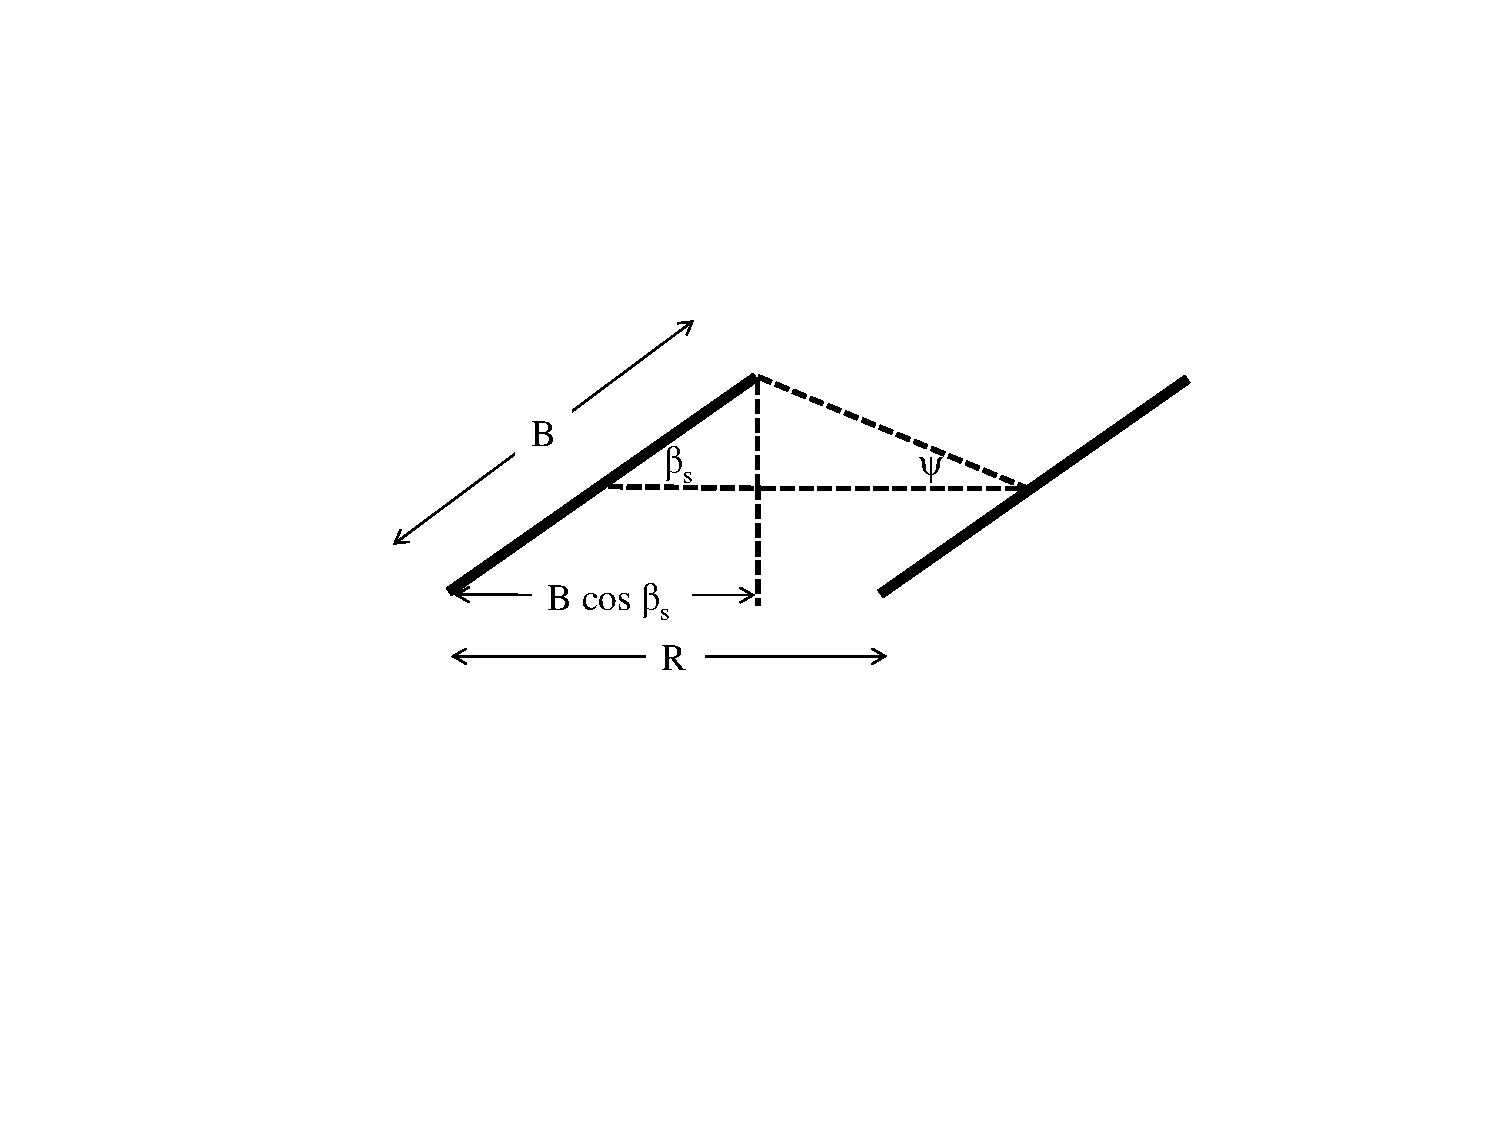
\includegraphics[scale=0.66]{self-shading-mask-angle}
\caption{Side View of Two Rows with Self-shading Mask Angle Variables}
\label{fig-selfshadingmaskangle}
\end{center}
\end{figure}

%mask_angle_calc_method is an input on the Array page
The mask angle is the minimum array tilt angle at which the view of the sky at a given point along the side of the row is obstructed by a neighboring row as shown in Figure~\ref{fig-selfshadingmaskangle} from \citet{passias1984}:
%pvsamv1 update 342
\begin{equation}
\psi = \arctan \frac{ (B)\sin\beta_s } { R - B\cos\beta_s }
\end{equation}

SAM uses the "worst case" approach described in \citep{deline2013b}, where the diffuse irradiance mask angle is calculated for the bottom of the array rather than averaged across the entire array.

%%%%%%%%%%%%%%%%%%%%%%%%%%%%%%%%%%%%%%%%%%%%%%%%%%
\section{Sky Diffuse POA Irradiance Reduction} \label{sec-selfshaddiff}

For the purposes of self-shading calculations, SAM assumes isotropic sky diffuse irradiance, so that the total horizontal diffuse irradiance $G_{dh}$ is:
%lib_pvshad update 168
\begin{equation}\label{eqn-selfshaddiffhor}
G_{dh} = G_d \left(\frac{2}{1+\cos\beta_s}\right)
\end{equation}

The beam horizontal irradiance is:
%lib_pvshad1 update 169
\begin{equation}
G_{bh} = E_b\cos Z 
\end{equation}

%Equations~\ref{eqn-selfshad-skydiff1}~-~\ref{eqn-selfshad-skydiff2} for calculating the reduction in sky diffuse POA irradiance are from \citep{passias1984}. The diffuse horizontal radiation $G_{dh}$ is from Equation~\ref{eqn-selfshaddiffhor}.

%The front row of modules (row nearest the sun) is not obscured, and the sky diffuse POA %irradiance on that row is a function of the surface tilt angle $\beta_s$:
%\begin{equation}\label{eqn-selfshad-skydiff1}
%G_d(\beta_s)=G_{dh}\cos^2\frac{\beta_s}{2}
%\end{equation}

The reduction in sky diffuse POA irradiance incident on the portion of the subarray shaded by neighboring rows is a function of the surface tilt angle $\beta_s$ and mask angle $\psi$ with a derating term $\frac{N_{rows}-1}{N_{rows}}$ for the number of interior rows in the array:
%lib_pvshad update 172
\begin{equation}\label{eqn-selfshad-skydiff2}
G_{sky,\text{red}} = G_d - G_{dh}\left(1 - \cos^2\frac{\psi}{2}\right)\frac{N_{rows} - 1}{N_{rows}}
\end{equation}

The sky diffuse shading factor:
%lib_pvshad update 173
\begin{equation}
S_{dss} = \frac{G_{sky,\text{red}}}{G_d}
\end{equation}

%%%%%%%%%%%%%%%%%%%%%%%%%%%%%%%%%%%%%%%%%%%%%%%%%%
\section{Ground Diffuse POA Irradiance Reduction} \label{sec-selfshadgndred}

%The equations for calculating the reduction in ground-reflected POA irradiance are from \citep{goswami1989}. The diffuse horizontal radiation $G_{dh}$ is from Equation~\ref{eqn-selfshaddiffhor}.

The first row in the subarray is not affected by self shading. The length of ground in front of each shaded row that reflects beam radiation onto the row, with $Y$ constrained to a minimum value of 0.00001:
%lib_pvshad update 182
\begin{equation}
Y = R - B \left(\frac{\sin( 180^\circ - \alpha - \beta_s )}{\sin\alpha} \right)
\end{equation}

The view factor on the first row $\mathit{F_1}$, and the beam and diffuse reflected component factors $\mathit{F_2}$ and $\mathit{F_3}$, respectively:
%lib_pvshad update 181, 184-185
\begin{align}
F_1 &= \mathit{\rho} \sin^2\frac{\beta_s}{2} \notag\\
F_2 &= \frac{\mathit{\rho}}{2} \left( 1 + \frac{Y}{B} - \sqrt{ \frac{Y^2}{B^2} - \frac{2Y}{B} \cos(180^\circ - \beta_s) + 1 }\right) \notag\\
F_3 &= \frac{\mathit{\rho}}{2} \left( 1 + \frac{R}{B} - \sqrt{ \frac{R^2}{B^2} - \frac{2R}{B} \cos(180^\circ - \beta_s) + 1 } \right)
\end{align}

The reduced ground-reflected diffuse POA irradiance on the entire subarray:
%lib_pvshad update 188
\begin{equation}
G_{gnd,red}=\left(\frac{F_1+F_2(N_{rows}-1)}{N_{rows}}\right)G_{bh}+\left(\frac{F_1+F_3(N_{rows}-1)}{N_{rows}}\right)G_{dh}
\end{equation}

The ground diffuse shading factor:
%pvsamv1 update 187-193
\[
S_{rss}=
 \left\{
     \begin{array}{ll}
      S_{rss} = \dfrac{G_{gnd,red}}{F_1 (G_{bh} +  G_{dh})}
      & \mbox{if $F_1 (G_{bh} + G_{dh}) > 0$}\\
      1 
      & \mbox{if $F_1 (G_{bh} + G_{dh}) \leq 0$}
    \end{array}
  \right.
\]

%%%%%%%%%%%%%%%%%%%%%%%%%%%%%%%%%%%%%%%%%%%%%%%%%%
\section{Shadow Dimensions}\label{sec-selfshaddim}

The shadow dimensions are defined by a shadow height  $H_S$ and shadow displacement $g$ as shown in Figure~\ref{fig-selfshaddimensions}. The equations are based on \citet{appelbaum1979}.

The shadow dimensions equations assume that a surface azimuth angle $\gamma_s$ of zero is for a south-facing surface in the northern hemisphere, and for a north-facing surface in the southern hemisphere. Because this differs from SAM's convention where $\gamma_s=0$ is for a north-facing surface and $\gamma_s=180^\circ$ is for a south-facing surface, the equations use the effective surface azimuth $\gamma_{s,eff}$:
%lib_pvshad update 366
\begin{equation}
\gamma_{s,eff} = \gamma - \gamma_s
\end{equation}
For an array that is not horizontal and for hours when the sun is up, the shaded portion of the array is:
%lib_pvshad update 372
%B defined above is equivalent to A in Applebaum equations
\begin{align} \label{eqn-pxpy}
P_y &= B \left(\cos\beta_s + \cos \gamma_{s,eff} \frac{\sin\beta_s}{\tan(90-Z)}\right)\notag\\
P_x &= B~\sin\beta_s \left(\frac{\sin\gamma_{s,eff}}{\tan(90-Z)}\right)
\end{align}

The shadow displacement $g$:
%lib_pvshad update 386
\begin{equation}\label{eqn-shadowdisplacement}
g=R\frac{P_x}{P_y}
\end{equation}

with the following constraints:
%lib_pvshad update 388
\[
g=
  \left\{
    \begin{array}{ll}
      \lvert g\rvert &  \mbox{when $g<0$}\\
      0 & \mbox{when $P_y=0$}\\
      0 & \mbox{when $M_{bottom}>M_{string}$}\\
      B & \mbox{when $g>B$}
    \end{array}
  \right.
\]

The shadow height $H_s$ in Figure~\ref{fig-selfshaddimensions} is:
%lib_pvshad update 403
\begin{equation} \label{eqn-shadowheight}
H_S=B \left(1-\frac{R}{P_y}\right)
\end{equation}
with the following constraints: 
\[
H_S=
  \left\{
    \begin{array}{ll}
      0                      & \mbox{when $P_y=0$}\\
      \lvert H_S \rvert & \mbox{when $g<0$}\\
      B                     & \mbox{when $H_s>B$}
    \end{array}
  \right.
\]

%S and X are inputs to the selfshade_dc_derate() function
When there is self shading, some fraction $X$ of each row in the subarray is shaded. In each row, a fraction $S$ of the number of modules along the side is of the row is shaded \citep{deline2013a}. The equations for $S$ and $X$ are from \citet{deline2013b}.

For landscape module orientation, the case where $H_S>W$ assumes complete shading even though in a given string, some modules will be completely shaded while others are only partly shaded ($\lceil...\rceil$ and $\lfloor...\rfloor$ indicate the ceiling and floor functions, respectively): 
%lib_pvshad update 418, 455 situation 1
\begin{equation}
X = \left\lceil\frac{H_S}{W}\right\rceil \dfrac{R-1}{R M_{side}}
\end{equation}
\[
S=
  \left\{
    \begin{array}{ll}
      \left\lceil \frac{H_S d}{W} \right
      \rceil d^{-1} 
      \left(1-\left\lfloor\dfrac{g}{L}\right\rfloor M^{-1}_{bottom}\right) 
      & \mbox{when $H_S\le W$ for a fixed subarray}\\
      1 
      & \mbox{when $H_S> W$, or for one-axis tracking}
    \end{array}
  \right.
\]

For portrait module orientation, the configuration shown in Figure~\ref{fig-selfshaddimensions}: 
%lib_pvshad update 433, 455  situation 2
\begin{equation}
X = \left\lceil \frac{H_S}{L} \right\rceil \dfrac{R-1}{R M_{side}}
\end{equation}
\[
S=
 \left\{
     \begin{array}{ll}
      1-\left\lfloor \dfrac{gd}{W}\right\rfloor \left(d M_{bottom}\right)^{-1} 
      & \mbox{for a fixed subarray}\\
      1 
      & \mbox{for one-axis tracking}
    \end{array}
  \right.
\]

%DELETE AFTER REVIEW
%\begin{align}
%S &= 1-\left\lfloor \frac{gd}{W}\right\rfloor \left(d N_{bottom}\right)^{-1} 
%\end{align}

SAM assumes that each module has three bypass diodes so that $d=3$ (See  Section~\ref{sec-selfshadgeom}).

%vertical strings not available as of SAM 2014.11.24
%For vertical strings and portrait module orientation ($\mathit{sor}=0$, %$\mathit{mor}=0$), this approximation assumes complete shading for modules on the %very edge of the array that may be only partially shaded: %situation 3
%\begin{align}
%X &= 1-\frac{\left\lfloor\lvert \frac{g}{W}\rvert\right\rfloor}{n} \notag\\
%S &= \left\lceil \frac{H_s}{L} \right\rceil \frac{r-1}{mr} 
%\end{align}

%For vertical strings and landscape module orientation ($\mathit{sor}=0$, %$\mathit{mor}=1$): %situation 4 
%\begin{align}\label{eqn-xs-landvert}
%X &= 1-\frac{\left\lfloor\lvert \frac{g}{L}\rvert\right\rfloor}{n} \notag\\
%S &= \left\lceil \frac{H_sd}{W} \right\rceil \frac{r-1}{dmr} 
%\end{align}

%%%%%%%%%%%%%%%%%%%%%%%%%%%%%%%%%%%%%%%%%%%%%%%%%%
\section{Beam Self-shading DC Loss Factor} \label{sec-selfshaddc}

The self-shading DC loss factor accounts for the reduction in beam POA irradiance caused by self shading. Its calculation is based on the proposed simplified analytical model from \citep{deline2013a} and requires the following variables:
\begin{itemize}
\item The shading fractions $S$ and $X$ described in Section~\ref{sec-selfshaddim}.
\item Fraction of solar irradiance reaching the shaded submodule $E_e$, which is a function of the reduction in diffuse POA irradiance from the sky and ground described in Section~\ref{sec-selfshaddiff}.
\item Submodule fill factor $\mathit{F}_{fill}$ determined from the module nameplate parameters.
\end{itemize}

The ratio of incident diffuse irradiance to total incident irradiance is a measure of the solar irradiance reaching the shaded submodule:
%lib_pvshade 469 (dbh_ratio in selfshade_dc_derate parameter list)
\begin{equation}
R_{dt} = \frac{G_{sky,red}+G_{gnd,red}}{G_b+G_{sky,red}+G_{gnd,red}}
\end{equation}

The fill factor depends on the photovoltaic module's rated maximum power, open-circuit voltage, and short-circuit current:
\begin{equation}
F_{fill}=\frac{P_{mp0}}{V_{oc0}I_{sc0}}
\end{equation}

The DC loss factor equation requires three coefficients, which were determined using the empirical analysis described in \citet{deline2013a}:
%lib_pvshade.cpp 263
\begin{align}
C_1 &= (109F_{fill}-54.3)e^{-4.5X} \notag\\
C_2 &= -6X^2+5X+0.28 \quad \text{(if $X>0.65$, set $X=0.65$)}\notag\\
C_3 &= \max\left[(-0.05R_{dt}-0.01)X+(0.85F_{fill}-0.7)R_{dt}-0.0855F_{fill}+0.05,R_{dt}-1\right]
\end{align}

The DC loss factor for fixed self shading is the ratio of the power of the shaded string to the power of the unshaded string. The choice of equation for calculating the DC loss factor equation depends on the magnitude of the shading factors:
\begin{itemize}
\item $F_{dc1}$ \quad Small $X$ and small $S$
\item $F_{dc2}$ \quad Large $X$
\item $F_{dc3}$ \quad Large $S$
\end{itemize}

The DC loss equations for each shade factor condition are:
%lib_pvshade.cpp 267-280
\begin{align}
F_{dc1} &= 1-C_1S^2-C_2S \notag\\ %eqn5
F_{dc2} &= 
\left\{
   \begin{array}{ll}
      \dfrac{X-S\left(1+0.5 d V^{-1}_{mp}\right)}{X} & \text{if $X>0$}\\
      0 & \text{if $X=0$}\\
   \end{array}
\right. \notag\\ %eqn9
F_{dc3} &= C_3\left(S-1\right)+R_{dt} %eqn10
\end{align}

SAM chooses the maximum of the three factors to calculate the system DC loss factor accounting for the reduction in beam POA irradiance due to self shading, and constrains the factor to between $0$ and $1$:
%lib_pvshade.cpp 274
\begin{equation}\label{eqn-selfshadedcderate}
F_{dcss}=X\max\left(F_{dc1},F_{dc2},F_{dc3}\right)+(1-X)
\end{equation}

%%%%%%%%%%%%%%%%%%%%%%%%%%%%%%%%%%%%%%%%%%%%%%%%%%
%%%%%%%%%%%%%%%%%%%%%%%%%%%%%%%%%%%%%%%%%%%%%%%%%%
\chapter{Module DC Output}\label{sec-module}

SAM uses one of four module submodels and one of three cell temperature submodels to calculate the DC power output of a single module in each subarray.  SAM's implementations of the submodels are effectively point-value efficiency models because SAM assumes that each subarray operates at its maximum power point (except with the mismatch option described in the next paragraph):
\begin{itemize}
\item The subarray maximum power point is determined by the maximum power point of a single module.
\item All modules in each subarray operate uniformly. SAM does not calculate module mismatch losses.
\end{itemize}

For an array with multiple subarrays and the CEC module submodel, SAM's optional PV subarray mismatch option adjusts the maximum power voltage to account for mismatch \textit{between subarrays} as described in Section~\ref{sec-mismatch}.

Calculating the module's DC output in a given hourly time step when the sun is up (see Section~\ref{sec-sunup}) is a two step process:
%cmod_pvsamv1.cpp 1466
\begin{enumerate}
\item Calculate the photovoltaic cell temperature. SAM assumes that the temperature of cells in all of the modules in each subarray is uniform.
\item Calculate the module's DC power output based on its physical characteristics, the effective irradiance, and cell temperature.
\end{enumerate}

Table~\ref{tab-modulevars} lists the input and output variables used by each of the module and cell temperature submodels described. Each submodel uses an additional set of input parameters as described in the submodel descriptions.

\begin{table}
\begin{center}
\caption{Module Submodel Variable Definitions}
\begin{tabular}{ll}
\midrule
Symbol & Description / \textbf{Name in SAM}\\
\midrule
\multicolumn{2}{c}{Inputs}\\
$G_b$ & effective beam irradiance \\
$G_d$ & effective sky diffuse irradiance \\
$G_r$ & effective ground-reflected irradiance  \\
$T_{dry}$ & ambient dry bulb temperature  \\
$v_w$ & wind speed from weather file \\
$Z$ & sun zenith angle \\
$h$ & elevation above sea level in meters from weather file \\
$\beta_s$ & subarray \textbf{tilt} angle \\
$\gamma_s$ & subarray \textbf{azimuth} angle \\
$\AOI$ & incidence angle \\
$\mathit{hr}$ & hour of day local time \\
\midrule
\multicolumn{2}{c}{Outputs}\\
$P_{dc}$ & module power \\
$V_{dc}$ & module voltage \\
$I_{dc}$ & module current  \\
$\eta_m$ & module efficiency \\
$V_{oc}$ & operating open circuit voltage  \\
$I_{sc}$ & operating closed circuit current \\
$T_c$ & cell temperature \\
\midrule
\end{tabular}
\label{tab-modulevars}
\end{center}
\end{table}

\section{Module Submodel Options}\label{sec-moduleoptions}

SAM calculates the a single photovoltaic module's DC output with one of the module submodels listed below, with descriptions from \citet{help-module} and \citet{blair2013}:

\begin{itemize}
\item \textbf{Simple Efficiency Module Model} (Section~\ref{sec-simplemodule}) is a simple representation of module performance that requires you to provide the module area, a set of conversion efficiency values, and temperature correction parameters. The simple efficiency model is the least accurate of the three models for predicting the performance of specific modules. It is useful for preliminary performance predictions before you have selected a specific module, and allows you to specify a module efficiency and temperature performance parameters, which is useful for analyses involving sensitivity or parametric analysis.
\item \textbf{California Energy Commission (CEC) Performance Model with Module Database} (Section~\ref{sec-cecmodule}) is an implementation of the six-parameter single-diode equivalent circuit model used in the CEC New Solar Homes Partneship Calculator \citep{gsc2014a}, and is an extension of the five-parameter model described in \citet{desoto2004a}. The model calculates the photovoltaic module hourly DC output using equations with parameters stored in SAM's CEC module library. The library contains data provided by the California Energy Commission \citep{gsc2014a} \citep{gsc2014b}.
\item \textbf{CEC Performance Model with User Entered Specifications}  (Section~\ref{sec-cecmodule}) is the same implementation as the CEC Performance Model with Module Database, but with a coefficient calculator \citep{dobos2012a} to calculate the model parameters from the standard module specifications provided on manufacturer data sheets. This makes it possible to use the six-parameter model for modules not included in the CEC module library.
\item \textbf{Sandia PV Array Performance Model with Module Database}  (Section~\ref{sec-sandiamodule}) is an implementation of the Sandia National Laboratories photovoltaic module and array performance model \citep{king2004}. The model calculates hourly efficiency values based on data measured from modules and arrays in realistic outdoor operating conditions. The database includes modules with different cell types, including crystalline silicon, and various thin film technologies.
\end{itemize}

In SSC, the \texttt{pvsamv1} input variable \texttt{module\_model} determines the module submodel as shown in Table~\ref{tab-modulesubmodels}.

\begin{table}
\begin{center}
\caption{Module Submodels in SSC}
\begin{tabular}{lc}
\midrule
Name in SAM & \texttt{module\_model} \\
\midrule
Simple Efficiency Module Model & 0 \\
CEC Performance Model with Module Database & 1 \\
CEC Performance Model with User Entered Specifications & 2 \\
Sandia PV Array Performance Model with Module Database & 3 \\
\hline
\end{tabular}
\label{tab-modulesubmodels}
\end{center}
\end{table}

\section{Cell Temperature Submodel Options}\label{sec-celltempoptions}

Each module submodel uses one of the cell temperature submodels shown in Table~\ref{tab-tempcorr} to calculate the photovoltaic cell temperature in a given hour. Each module submodel uses a single cell temperature submodel, except for the CEC module model with database parameters, which offers two cell temperature submodel options.

\begin{table}
\begin{center}
\caption{Cell Temperature Submodels}
\begin{tabular}{lll}
\midrule
Module Model & Temperature Model & Section\\
\midrule
Simple efficiency & Sandia & \ref{sec-tcsandia}\\
Sandia & Sandia & \ref{sec-tcsandia} \\
CEC with database parameters & NOCT or Heat Transfer & \ref{sec-tcnoct} or \ref{sec-tcheattransfer}\\
CEC with user-specified parameters & NOCT & \ref{sec-tcnoct}\\
\hline
\end{tabular}
\label{tab-tempcorr}
\end{center}
\end{table}

As described above, in each hourly time step, SAM calls the appropriate cell temperature submodel once before calling the module submodel. When the subarray mismatch option (Section~\ref{sec-mismatch}) is enabled, it also calls the cell temperature submodel as part of that set of calculations.

\section{Module Degradation}

SAM's module submodels calculate the DC power output of a single module in a single hourly time step. For a given simulation, SAM runs the module submodel 8,760 times to calculate the output over a single year. Because the model calculates the output in a single year, it does not have the information required to model degradation of module output over a number of years of operation.

SAM's photovoltaic performance model calculates the hourly AC output of the photovoltaic system. Its financial models add up these 8,760 hourly values to calculate the system's total AC output in one year, and treat this value as the system's total output in the first year of the system's operation.

The financial models use a lifetime in years and annual degradation factor to calculate the system's output in the second year and later for cash flow calculations. This degradation factor can approximate the impact of module degradation on the performance of a photovoltaic system. However, because the degradation factor applies to the total annual \textit{AC output} of the system, it only very roughly represents module degradation. In an actual system, module degradation reduces the array's \textit{DC output}, and this reduction can affect inverter sizing decisions in a way that SAM cannot model.

If the weather file for a given analysis contains typical-year data (rather than data for a specific year), using the AC degradation factor to represent module degradation is further complicated by the fact that the solar resource input to the module model represents the resource over a multi-year period.

%%%%%%%%%%%%%%%%%%%%%%%%%%%%%%%%%%%%%%%%%%%%%%%%%%
%%%%%%%%%%%%%%%%%%%%%%%%%%%%%%%%%%%%%%%%%%%%%%%%%%
\section{Sandia Module Model}\label{sec-sandiamodule}

SAM's Sandia Module Model (see Section~\ref{sec-moduleoptions}) is an implementation of the empirical model of a photovoltaic module described in \citet{king2004}. 

For a description of the Sandia cell temperature model, see Section~\ref{sec-tcsandia}.

The Sandia module model uses the module parameters in Table~\ref{tab-sandiamodulevars} along with the general module input variables in Table~\ref{tab-modulevars}. The parameters in Table~\ref{tab-sandiamodulevars} are from the Sandia module database maintained by Sandia National Laboratories \citep{sandia-testeval}.  In SAM, the parameters are stored in the Sandia module library \citep{help-libraries}. In SSC, the implementation of the Sandia module model described here is part of the \texttt{pvsamv1} module and does not include a parameter library (See Section~\ref{sec-libraries}).

%%
% How does SAM use fill factor? See cmod_pvsamv1.cpp 769, and Equation 6 in King 2004.

\begin{table}
\begin{center}
\caption{Sandia Module Model Variable Definitions}
\begin{tabular}{lll}
\midrule
Symbol & Description / \textbf{Name in SAM} & Name in SSC \\
\midrule
\multicolumn{3}{c}{Inputs}\\
$V_{mp,ref}$ & reference \textbf{Max Power Voltage} &\texttt{snl\_vmpo} \\
$I_{mp,ref}$ & reference \textbf{Max Power Current} & \texttt{snl\_i\_mpo} \\
$V_{oc,ref}$ & reference \textbf{Open Circuit Voltage} & \texttt{snl\_voco} \\
$I_{sc,ref}$ & reference \textbf{Short Circuit Current} & \texttt{snl\_isco} \\
$\alpha_{sc,ref}$ & short circuit temperature coefficient & \texttt{snl\_aisc} \\
$\beta_{oc,ref}$ & open circuit temperature coefficient & \texttt{snl\_bvoco} \\
$\beta_{mp,ref}$ & maximum power voltage temperature coefficient & \texttt{snl\_bvmpo} \\
$\gamma_{mp,ref}$ & maximum power temperature coefficient & \texttt{snl\_aimp} \\
$M_{\beta oc}$ & relates $\beta_{oc,ref}$ to effective irradiance& \texttt{snl\_mbvoc} \\
$M_{\beta mp}$ & relates $\beta_{mp,ref}$ to effective irradiance& \texttt{snl\_mbvmp} \\
$s$ & number of cells in series & \texttt{snl\_series\_cells} \\
$C_0$, $C_1$ & coefficients relating $I_{mp}$ to $G$ & \texttt{snl\_c0}, \texttt{snl\_c1} \\
$C_2$, $C_3$ & coefficients relating $V_{mp}$ to $G$ & \texttt{snl\_c2}, \texttt{snl\_c3} \\
$C_4$, $C_5$ & coefficients relating $I_x$ to $G$ & \texttt{snl\_c4}, \texttt{snl\_c5} \\
$C_6$, $C_7$ & coefficients relating $I_{xx}$ to $G$ & \texttt{snl\_c6}, \texttt{snl\_c7} \\
$n$ & diode factor & \texttt{snl\_n} \\
$f_d$ & fraction of diffuse irradiance used by module & \texttt{snl\_fd} \\
$a_{0...4}$ & air mass coefficients 0...4 & \texttt{snl\_a[\textit{0...4}]} \\
$b_{0...5}$ & incidence angle modifier coefficients 0...5 & \texttt{snl\_b[\textit{0...5}]} 
\\
\midrule
\multicolumn{3}{c}{Output}\\
$P_{dc,m}$ & module DC output power & \\
\hline
\end{tabular}
\label{tab-sandiamodulevars}
\end{center}
\end{table}

The reference conditions for the Sandia module model parameters are total incident irradiance of 1,000 W/m$^2$ and reference cell temperature of 25\degree C. 

When you select a module on SAM's Module input page for the \textbf{Sandia PV Array Performance Model with Module Database}, SAM displays some of the module's reference parameters in Table~\ref{tab-sandiamodulevars} from the Sandia Module library as uneditable values. You can use SAM's library editor to see a complete list of the module parameters or to modify parameter values \citep{help-libraries}.

The absolute air mass is a relative measure of the optical path length that sunlight travels through the atmosphere and depends on the sun zenith angle in degrees (Section~\ref{sec-sunangles}) and the elevation above sea level ($AM=1$ at sea level with the sun directly overhead):
%lib_sandia.cpp 245, 154
\begin{equation}\label{eqn-sandiaam}
AM = \left[ \cos(\frac{\pi}{180} Z ) + 0.5057 (96.08 - Z)^{-1.634} \right]^{-1} e^{-0.0001184 h}
\end{equation}

The $F_1$ polynomial relates the spectral effects on $I_{sc}$ to the variation of air mass over the day:
%lib_sandia.cpp 248, 136
\begin{equation}
F_1 = a_0 + a_1 AM + a_2 AM^2 + a_3 AM^3 + a_4 AM^4
\end{equation}

The $F_2$ polynomial relates the optical effects on $I_{sc}$ to the angle of incidence $\AOI$ (Section~\ref{sec-theta}):
%lib_sandia.cpp 251, 118
\begin{equation}
F_2 = b_0 + b_1\AOI
		+ b_2\AOI^2
		+ b_3\AOI^3
		+ b_4\AOI^4
		+ b_5\AOI^5
\end{equation}

The short circuit current is a function of the cell temperature (Section~\ref{sec-tcsandia}), effective irradiance (Section~\ref{sec-effectiveirradiance}) and the short circuit temperature coefficient in A/\degree C. The diffuse utilization factor $F_d$ is one of the parameters from the Sandia module library, and is equal to one for flat plate modules:
%lib_sandia.cpp 254, 96
\begin{equation}
I_{sc} = I_{sc,ref} F_1 \left( \frac{G_b F_2 + f_d (G_d+G_r)}{1000} \right) \left[1+\alpha_{sc,ref} (T_c-25)\right]
\end{equation}

The effective irradiance on the module surface to which the cells respond:
%lib_sandia.cpp 256, 169
\begin{equation}
E_e = \frac{I_{sc}}{I_{sc,ref} \left[1 + \alpha_{sc,ref} (T_c - 25)\right]}
\end{equation}

The current at the maximum power point:
%lib_sandia.cpp 257, 107
\begin{equation}
I_{mp} = I_{mp,ref} (C_0 E_e + C_1 E_e^2) \left[1 + \alpha_{sc,ref} (T_c - 25)\right]
\end{equation}

The following two intermediate values are required for the maximum power voltage equations:
%lib_sandia.cpp 18, 45
\begin{align}
\Delta T_c &= n \left(\frac{1.38066\times10^{-23} (T_c + 273.15)}{1.60218\times10^{-19}}\right) \notag\\
%\beta_{oc} & = \beta_{oc,ref} + M_{\beta oc} (1 - E_e) \notag\\
\beta_{mp} & = \beta_{mp,ref} + M_{\beta mp} (1 - E_e)
\end{align}

%The open circuit voltage is zero if $E_e \leq 0$. Otherwise:
%%lib_sandia.cpp 263, 18
\begin{equation}
V_{oc} = V_{oc,ref}+ s~\Delta T_c \ln(E_e)+ \beta_{oc} (T_c - 25)
\end{equation}

The voltage at the maximum power point is zero if $E_e \leq 0$. Otherwise:
%lib_sandia.cpp 266, 48
\begin{equation}
V_{mp} = V_{mp,ref} +
 C_2~s~\Delta T_c~\ln(E_e) +
 C_3~s~\left[\Delta T_c \ln(E_e)\right]^2 +
 \beta_{mp} (T_c - 25)
\end{equation}

The module's DC power output is at the maximum power point:
%lib_sandia.cpp 295
\begin{equation}
P_{dc,m} = V_{mp}~I_{mp}
\end{equation}

%%%%%%%%%%%%%%%%%%%%%%%%%%%%%%%%%%%%%%%%%%%%%%%%%%
%%%%%%%%%%%%%%%%%%%%%%%%%%%%%%%%%%%%%%%%%%%%%%%%%%
\section{CEC Module Model}\label{sec-cecmodule}

SAM's CEC Module Model  (see Section~\ref{sec-moduleoptions}) is an implementation of the single-diode equivalent circuit model of a photovoltaic module described in \citet{desoto2004a}, and with more detail in \citet{desoto2004b}. It is also described in Section 23.2 of  \citet{duffie2013}.

SAM includes two options for the model (see Section~\ref{sec-module}): It may use a set of reference parameters from the CEC module library with data provided by the California Energy Commission \citep{gsc2014a}, or a set of reference parameters generated by SAM's coefficient generator from module specifications that you provide as input to the model. The equations described in this section are for the module's DC output, not for the module coefficients. For a description of the coefficient generator equations, see \citet{dobos2012a}. 

Table~\ref{tab-cecmodulevars} shows the five module specifications and six parameters that are input variables specific to the CEC module model. The model also uses the general module input variables in Table~\ref{tab-modulevars}.

In SSC, the implementation of the CEC module model described here is part of the \texttt{pvsamv1} module. The coefficient generator is available in SSC as a separate compute module called \texttt{6parsolve}.

\begin{table}
\begin{center}
\caption{CEC Module Model Variable Definitions}
\begin{tabular}{lll}
\midrule
Symbol & Description / \textbf{Name in SAM} & Name in SSC \\
\midrule
\multicolumn{3}{c}{Inputs}\\
$I_{mp,ref}$ & reference \textbf{Max Power Current} & \texttt{cec\_i\_mp\_ref} \\
$V_{oc,ref}$ & reference \textbf{Open Circuit Voltage} & \texttt{cec\_v\_oc\_ref} \\
$I_{sc,ref}$ & reference \textbf{Short Circuit Current} & \texttt{cec\_i\_sc\_ref} \\
$\alpha_{sc,ref}$ & short circuit current temperature coefficient (A/\degree C) & \texttt{cec\_alpha\_sc} \\
$\beta_{oc,ref}$ & open circuit voltage temperature coefficient (V/\degree C) & \texttt{cec\_beta\_oc} \\
$I_{L,ref}$ & reference light current, \textbf{I\_L\_ref} & \texttt{cec\_i\_l\_ref} \\
$I_{o,ref}$ & reference diode saturation current, \textbf{I\_o\_ref} & \texttt{cec\_i\_o\_ref} \\
$R_{s,ref}$ & reference series resistance, \textbf{R\_s} & \texttt{cec\_r\_s\_ref} \\
$a_{ref}$ & reference ideality factor, \textbf{A\_ref} & \texttt{cec\_a\_ref} \\
$R_{sh,ref}$ & reference shunt resistance \textbf{R\_sh\_ref}& \texttt{cec\_r\_sh\_ref} \\
$\mathit{adjust}$ & temperature coefficient adjustment factor & \texttt{cec\_adjust} \\
\midrule
\multicolumn{3}{c}{Output}\\
$P_{dc,m}$ & module DC output power & \\
\hline
\end{tabular}
\label{tab-cecmodulevars}
\end{center}
\end{table}

The reference conditions for the CEC module model parameters are total incident irradiance of 1,000 W/m$^2$ and reference cell temperature of 25\degree C. 

When you select a module on SAM's Module input page for the \textbf{CEC Performance Model with Module Database}, SAM displays the module's reference parameters shown in Table~\ref{tab-cecmodulevars} from the CEC Module library as uneditable values. You can use SAM's library editor to modify reference parameter values for a module  \citep{help-libraries}.

The five-parameter single-diode equivalent circuit equation for the module current $I$ at a given voltage $V$ is:
\begin{equation}\label{eqn-cec5par}
I = I_L - I_o \left[ \exp\left(  \frac{V+IR_S}{a} \right) -1 \right] - \frac{V + IR_S}{R_{sh}}
\end{equation}

The temperature coefficient of short circuit current $\mu_{isc}$ and open circuit voltage $\beta_{voc}$ in the model are adjusted from the reference coefficients using a sixth parameter, $\mathit{adjust}$, which may be either from the CEC module library, or calculated by SAM's coefficient generator:
%lib_cec6par.cpp 302
\begin{align}
\mu_{isc} & = \alpha_{sc,ref} \left( 1-\frac{\mathit{adjust}}{100}\right) \notag\\
\beta_{voc} & = \beta_{oc,ref} \left( 1+\frac{\mathit{adjust}}{100}\right) 
\end{align}

The global effective irradiance at the top of the module cover:
\begin{equation}
G = G_b + G_d + G_r
\end{equation}

Equations for the transmittance through the module cover use three constants:
%lib_cec6par.cpp 210
\begin{align}\label{eqn-coverproperties}
n & = 1.526 \quad\text{(refractive index of glass)} \notag\\
L & = 0.002 \quad\text{(thickness of glass cover in meters)} \notag\\
K &= 4 \quad\text{(proportionality constant in meters$^{-1}$)}
\end{align}

%lib_cec6par.cpp 230
The angle of refraction, assuming that the refractive index of air is one:
\begin{equation}
\theta_r = \arcsin\left(\frac{1}{n} \sin \AOI \right)
\end{equation}

The transmittance as a function of incidence angle $\theta_i$ in radians:
%lib_cec6par.cpp 232
\begin{equation}\label{eqn-transmittance}
\tau(\theta) = e^{-K L/\cos \theta_r} \left[1 - \frac{1}{2} \left( \frac{\sin^2(\theta_r-\theta_i)}{\sin^2(\theta_r+\theta_i)}
			+ \frac{\tan^2(\theta_r-\theta_i)}{\tan^2(\theta_r+\theta_i)} \right)\right] 
\end{equation}

The incidence angle for the sky diffuse and ground-reflected components of the effective irradiance:
%lib_cec6par.cpp 265
\begin{align}
\theta_d &= 59.7 - 0.1388 \beta + 0.001497 \beta^2 \quad\text{(sky diffuse angle)} \notag\\
\theta_g &= 90 - 0.5788 \beta  + 0.002693 \beta^2 \quad\text{(ground-reflected diffuse angle)} 
\end{align}

The transmittance for each component of the effective irradiance is calculated using Equation~\ref{eqn-transmittance} with the module cover properties in Equation~\ref{eqn-coverproperties} and the following incidence angle values:
%lib_cec6par.cpp 258, De Soto Eq 13
\begin{align}
(\tau\alpha)_n: \theta_i &= 1 \quad\text{(surface normal)} \notag\\
(\tau\alpha)_b: \theta_i &= \theta \quad\text{(beam)} \notag\\
(\tau\alpha)_d: \theta_i &= \theta_d \quad\text{(sky diffuse)} \notag\\
(\tau\alpha)_g: \theta_i &= \theta_g  \quad\text{(ground diffuse)}
\end{align}

Note that $(\tau\alpha)_n$ is set to 1 degree (a very small number) instead of zero to avoid potential divide-by-zero errors.

The incidence angle modifier for each component of the effective irradiance is then:
%lib_cec6par.cpp 258, De Soto Eq 13
\begin{align}
K_{\tau\alpha,b} = \frac{(\tau\alpha)_b}{(\tau\alpha)_n} \notag\\
K_{\tau\alpha,d} = \frac{(\tau\alpha)_d}{(\tau\alpha)_n} \notag\\
K_{\tau\alpha,g} = \frac{(\tau\alpha)_g}{(\tau\alpha)_n}
\end{align}

The irradiance absorbed by the photovoltaic cell is:
%lib_cec6par.cpp 310, De Soto Eq 19
\begin{equation}
G_0 = G_b K_{\tau\alpha,b} + G_d K_{\tau\alpha,d} + G_r K_{\tau\alpha,g}
\end{equation}

%lib_cec6par.cpp 318
The model limits sun zenith angle, setting its value to the minimum or maximum when it is exceeded:
\begin{equation}
0 < Z < 86\degree  
\end{equation}

The transmittance-absorptance product:
%lib_cec6par.cpp 325
\begin{equation}
\tau\alpha = 0.9 \frac{G_0}{G}
\end{equation}

The air mass, with an exponential correction factor adapted from the Sandia model for elevation above sea level:
%lib_cec6par.cpp 332, De Soto Eq 18
\begin{equation}\label{eqn-cecam}
\textit{AM} = \left[\cos\left( \frac{\pi}{180}Z \right)+0.5057(96.080-Z)^{-1.634} \right]^{-1} e^{-0.0001184\mathit{h}}
\end{equation}

The air mass modifier $M$ accounts for the effect of air mass on spectral distribution, and is from \citet{king2004} with coefficients for polycrystalline cells:
%lib_cec6par.cpp 334, De Soto Eq 17
\begin{align}
a_0 &= 0.918093 \notag\\
a_1 &= 0.086257 \notag\\
a_2 &= -0.024459 \notag\\
a_3 &= 0.002816 \notag\\
a_4 &= -0.000126 \notag\\
\textit{M} &= a_0 + a_1 \mathit{AM} + a_2 \mathit{AM}^2 + a_3\mathit{AM}^3+ a_4\mathit{AM}^4
\end{align}

The adjusted effective transmitted irradiance:
%lib_cec6par.cpp 335
\begin{equation}\label{eqn-effectivetransmittedirradiance}
G =  MG_0
\end{equation}

%lib_cec6par.cpp 338
The module DC output is only calculated when $G>1$.

The cell temperature $T_c$ for the CEC module model is calculated using either the NOCT cell temperature model (Section~\ref{sec-tcnoct}) or the heat transfer cell temperature model (Section~\ref{sec-tcheattransfer}). For the next set of equations, the cell temperature is in Kelvin, and the reference cell temperature of $25\degree C$ in Kelvin is $25\degree \text{C} + 273.15 \text{K} = 298.15 \text{K}$.

The light current $I_L$:
%lib_cec6par.cpp 343
\begin{equation}\label{eqn-lightcurrent}
I_L = \frac{G}{1000}\left[I_{L,ref} + \mu_{I,sc} (T_c - 298.15 )\right]
\end{equation}

%lib_cec6par.cpp 220
The diode reverse saturation current $I_o$, assuming a reference band-gap energy of silicon of 1.12 eV:
%lib_cec6par.cpp 347
\begin{align}
k &= 8.618 \times 10^{-5} &\quad\text{Boltzmann constant in eV/K} \notag\\
E_{bg} &= 1.12 \left[1-0.0002677(T_c-T_{c,ref})\right] &\quad\text{cell material band-gap energy in eV}\notag\\
I_o &= I_{o,ref} \left( \frac{T_c}{298.15} \right)^3 \exp\left[ \frac{1}{k} \left( \frac{1.12}{T_{c,ref}} - \frac{E_{bg}}{T_c} \right) \right] &
\end{align}

At the open circuit voltage $V_{oc}$, $I=0$, and Equation~\ref{eqn-cec5par} reduces to:
%lib_cec6par.cpp 193
\begin{equation}\label{eqn-cec5parvoc}
I = I_L - I_o \left[ \exp\left(  \frac{V_{oc}+IR_S}{a} \right) -1 \right] - \frac{V_{oc}}{R_{sh}}
\end{equation}

SAM uses the bisection method to solve Equation~\ref{eqn-cec5parvoc} for $V_{oc}$ with the reference open circuit voltage $V_{oc,ref}$ as an initial guess and the following parameter values:
%lib_cec6par.cpp 351
\begin{align} 
a &= a_{ref} \frac{T_c}{T_{c,ref}} \notag\\
R_{sh} &= R_{sh,ref} \frac{1000}{G}
\end{align}

The short circuit current:
%lib_cec6par.cpp 352
\begin{equation} \label{eqn-cecisc}
I_{sc} = \frac{I_L }{1+\frac{R_{s,ref}}{R_sh}}
\end{equation}

For the CEC module model, SAM can calculate the module operating voltage either using the string mismatch equations described in Section~\ref{sec-mismatch}, or the equations described below.%not clear where module_voltage is calculated without mismatch option

%The voltage at maximum power:
%%lib_cec6par.cpp 385
%\begin{equation}
%V_{mp} = \frac{1}{2} \left[ V_{mp,ref} + \beta_{voc} (T_c - T_{c,ref}) \right]
%\end{equation}

%lib_cec6par.cpp 393
For the current at maximum power $I_{mp}$, SAM uses Newton's method to find a solution of Equation~\ref{eqn-cec5par} using the calculated values for $I_L$, $I_o$, $a$, and $R_{sh}$ at the maximum power point voltage. Because the effect of series resistance on the maximum power point is relatively small, for $R_S$, the model uses the reference value so that $R_S=R_{S,ref}$. Also, $I_L$ from Equation~\ref{eqn-lightcurrent} is multiplied by a factor of 0.9.

%lib_cec6par.cpp 367
For systems with one subarray, or for systems with more than one subarray with the subarray mismatch option disabled, SAM calculates the maximum power point voltage using a golden section search to determine the voltage between 0 and $V_{oc}$ that results in the maximum power given the current at maximum power.

%lib_cec6par.cpp 403
For systems with more than one subarray and the subarray mismatch option enabled (Section~\ref{sec-mismatch}, SAM sets the maximum power voltage to the value calculated by the mismatch algorithm.

The module DC output is the power at maximum power:
%lib_cec6par.cpp 391, 407
\begin{equation}
P_{dc,m} = V_{mp}~I_{mp}
\end{equation}

%%%%%%%%%%%%%%%%%%%%%%%%%%%%%%%%%%%%%%%%%%%%%%%%%%
%%%%%%%%%%%%%%%%%%%%%%%%%%%%%%%%%%%%%%%%%%%%%%%%%%
\section{Simple Efficiency Module Model}\label{sec-simplemodule}

SAM's Simple Efficiency Module Model  (see Section~\ref{sec-moduleoptions}) is a basic single point efficiency representation of a photovoltaic module that uses an efficiency table and the Sandia cell temperature model (Section~\ref{sec-tcsandia}) to calculate the module's DC power output.

The simple efficiency module model uses the module parameters shown in Table~\ref{tab-spemodulevars} along with the general module input variables in Table~\ref{tab-modulevars}. Note that the model does not use the reference parameters $V_{mp,ref}$ and $V_{oc,ref}$. Those values are required by the sizing algorithm that is part of SAM's user interface (Section~\ref{sec-sizing}).

The cell temperature parameters $a$, $b$, and $\Delta T$ depend on the \textbf{Module Structure and Mounting} option (\texttt{spe\_module\_structure} in SSC) as listed in Table~\ref{tab-sandiamodstruct}. Note that the ``use database values" option is not available for the simple efficiency module model, so that  $\mathtt{spe\_module\_structure}=0$ is for the ``glass/cell/polymer sheet - open rack" option instead of the``use database option" as shown in the table for \texttt{snl\_module\_structure}.

\begin{table}
\begin{center}
\caption{Simple Efficiency Module Model Variable Definitions}
\begin{tabular}{lll}
\midrule
Symbol & Description / \textbf{Name in SAM} & Name in SSC \\
\midrule
\multicolumn{3}{c}{Inputs}\\
$V_{mp,ref}$ & reference \textbf{Maximum Power Voltage} & - \\
$V_{oc,ref}$ & reference \textbf{Open Circuit Voltage} & - \\
$A_m$ & module \textbf{Area} & \texttt{spe\_area} \\
$\gamma_{mp,ref}$ & maximum power \textbf{Temperature Coefficient} & \texttt{spe\_temp\_coeff} \\
$a$ & Sandia temperature parameter \textbf{a} & \texttt{spe\_a} \\
$b$ & Sandia temperature parameter \textbf{b} & \texttt{spe\_b} \\
$\Delta T$ & Sandia temperature parameter \textbf{dT} & \texttt{spe\_dT} \\
$G_{0...4}$ & radiation values in efficiency table & \texttt{spe\_rad[\textit{0...4}]} \\
$G_{ref}$ & reference radiation value from efficiency table & \texttt{spe\_reference} \\
$\eta_{0...4}$ & module efficiency values in efficiency table & \texttt{spe\_eff[\textit{0...4}]} \\
$f_d$ & \textbf{Diffuse utilization factor} & \texttt{spe\_fd} \\
\midrule
\multicolumn{3}{c}{Output}\\
$P_{dc,m}$ & module DC output power & \\
\hline
\end{tabular}
\label{tab-spemodulevars}
\end{center}
\end{table}

The reference irradiance condition for the simple efficiency module model is the value that you specify, typically 1,000 W/m$^2$. The reference cell temperature is 25\degree C. 

The effective total irradiance (the diffuse utilization factor $F_d$ is adapted from the Sandia module model, and is equal to one for flat plate modules):
%lib_pvmodel.cpp 101
\begin{equation}
G = G_b + f_d(G_d+G_r)
\end{equation}

%lib_pvmodel.cpp 102
SAM determines the module's conversion efficiency $\eta_m$ by using linear interpolation on the radiation and efficiency values in the efficiency table to estimate the conversion efficiency at the effective total irradiance value $G$.

The module's DC power output:
%lib_pvmodel.cpp 103
\begin{equation}
P_{dc,m} = G \eta_m A_m \frac{\gamma_{mp,ref}}{100} (T_c - 25)
\end{equation}


\section{NOCT Cell Temperature Model} \label{sec-tcnoct}

The NOCT photovoltaic cell temperature model is from Chapter 23.3 of \citet{duffie2013}, also described in \citet{desoto2004b}. In SAM's implementation of the model, it is available with the \textbf{CEC Performance Model with Module Database} module model on the Module input page as the \textbf{NOCT cell temp model} option ($\mathtt{cec\_temp\_corr\_mode}=0$ in SSC \texttt{pvsamv1}).

\begin{table}
\begin{center}
\caption{NOCT Cell Temperature Model Variable Definitions}
\begin{tabular}{lll}
\midrule
Symbol & Description / \textbf{Name in SAM} & Name in SSC \\
\midrule
\multicolumn{3}{c}{Inputs}\\
$G$ & effective irradiance transmitted to the photovoltaic cell & - \\
$\tau \alpha$ & effective transmittance-absorbtance product & - \\
$v_{w}$ & wind speed from weather file & - \\
- & \textbf{Array height} & \texttt{cec\_height} \\
- & \textbf{Mounting standoff} & \texttt{cec\_standoff} \\
$T_{noct}$ & module NOCT temperature rating & \texttt{6par\_tnoct} \\
$I_{mp}$ & module maximum power current rating & \texttt{6par\_imp} \\
$V_{mp}$ & module maximum power voltage rating & \texttt{6par\_vmp} \\
$A_m$ & module area in meters & \texttt{6par\_area} \\
\midrule
\multicolumn{3}{c}{Output}\\
$T_c$ & cell temperature & \texttt{hourly\_subarray[\textit{n}]\_celltemp} \\
\hline
\end{tabular}
\label{tab-tempnoct}
\end{center}
\end{table}

The cell temperature is only calculated when the effective transmitted irradiance from Equation~\ref{eqn-effectivetransmittedirradiance} is greater than zero, $G>0$.

The reference module efficiency is based on the module specifications at 1,000 W/m$^2$ incident irradiance:
%lib_cec6par.cpp 469
\begin{equation}
\eta_{ref} = \frac{I_{mp} V_{mp}}{1000 A_m}
\end{equation}

The wind speed adjusted for height above the ground depends on the \textbf{Array height} option on the Module page (\texttt{cec\_height} in SSC):
%lib_cec6par.cpp 472
\begin{equation}
v_{w,adj} = \left\{
\begin{array}{ll}
0.51 v_{w} & \text{one story or lower} \\
0.61 v_{w} & \text{two stories or higher} \\
\end{array}
\right.
\end{equation}

The NOCT adjusted for mounting stand-off type depends on the \textbf{Mounting standoff} option on the Module page (\texttt{cec\_standoff} in SSC):
%lib_cec6par.cpp 476, cmod_pvsamv1.cpp 778
\begin{equation}
T_{noct,adj} =\left\{
\begin{array}{ll}
T_{noct} + 2  & \text{building integrated, greater than 3.5 in, or ground/rack mounted}\\
T_{noct} + 2 & \text{2.5 to 3.5 in} \\
T_{noct} + 6 & \text{1.5 to 2.5 in} \\
T_{noct} + 11 & \text{0.5 to 1.5 in} \\
T_{noct} + 18 & \text{less than 0.5 in} \\
\end{array}
\right.
\end{equation}

The cell temperature in degrees Celsius (\degree C):
%lib_cec6par.cpp 477
\begin{equation}
T_c = T_a + \frac{G}{800} \left(T_{noct,adj} - 20 \right) \left(1-\frac{\eta_{ref}}{\tau \alpha}\right) \frac{9.5}{5.7+3.8v_{w,adj}}
\end{equation}

\section{Heat Transfer Cell Temperature Model}\label{sec-tcheattransfer}

The heat transfer cell temperature model is from the work described in \citet{neises2011}, with model descriptions in Chapters 4 and 5, and an implementation in FORTRAN in Appendix H. SAM's model is adapted from the FORTRAN implementation, and its description is omitted from this section because of its length.

In SAM, the heat transfer cell temperature model is available with the \textbf{CEC Performance Model with Module Database} module model on the Module input page as the \textbf{Mounting specific cell temp model} option ($\mathtt{cec\_temp\_corr\_mode}=1$ in SSC \texttt{pvsamv1}).

%inputs cmod_pvsamv1.cpp 802
\begin{table}
\begin{center}
\caption{Heat Transfer Cell Temperature Model Variable Definitions}
\begin{tabular}{ll}
\midrule
Description / \textbf{Name in SAM} & Name in SSC \\
\midrule
\multicolumn{2}{c}{Inputs}\\
\textbf{Mounting Configuration} & \texttt{cec\_mounting\_config} \\ 
\textbf{Heat Transfer Dimensions} & \texttt{cec\_heat\_transfer} \\ 
\textbf{Mounting Structure Orientation} & \texttt{cec\_mounting\_orientation} \\ 
\textbf{Module Width} & \texttt{cec\_module\_width} \\ 
\textbf{Module Length} & \texttt{cec\_module\_length} \\ 
\textbf{Rows of modules in array} & \texttt{cec\_array\_rows} \\ 
\textbf{Columns of modules in array} & \texttt{cec\_array\_cols} \\ 
\textbf{Temperature behind the module} & \texttt{cec\_backside\_temp} \\ 
\textbf{Gap Spacing} & \texttt{cec\_gap\_spacing} \\ 
\midrule
\multicolumn{2}{c}{Output}\\
cell temperature & \texttt{hourly\_subarray[\textit{n}]\_celltemp} \\
\hline
\end{tabular}
\label{tab-tempheattransfer}
\end{center}
\end{table}

\section{Sandia Cell Temperature Model}\label{sec-tcsandia}

The Sandia photovoltaic cell temperature model is the cell temperature model described in \citet{king2004} as part of the Sandia photovoltaic array performance model. In SAM's implementation of the model, it is available with the \textbf{Sandia PV Array Performance Model with Module Database} module model on the Module input page.

The Sandia cell temperature model requires the effective incident irradiance and three empirical parameters from the Sandia module library, which stores data provided by the Sandia National Laboratories Photovoltaic Test and Evaluation program \citep{sandia-testeval}.

\begin{table}
\begin{center}
\caption{Sandia Cell Temperature Model Variable Definitions}
\begin{tabular}{lll}
\midrule
Symbol & Description / \textbf{Name in SAM} & Name in SSC \\
\midrule
\multicolumn{3}{c}{Inputs}\\
$G_b$ & effective beam irradiance & - \\
$G_d$ & effective sky diffuse irradiance & - \\
$G_r$ & effective ground-reflected irradiance & - \\
$v_{w}$ & wind speed from weather file & - \\
$T_{a}$ & ambient temperature from weather file & - \\
$a$ & Temperature coefficient \textbf{a} & \texttt{snl\_a} or \texttt{snl\_ref\_a}\\
$b$ &  Temperature coefficient \textbf{b} & \texttt{snl\_b} or \texttt{snl\_ref\_b}\\
$\Delta T$ & Temperature coefficent \textbf{dT} & \texttt{snl\_dtc} or \texttt{snl\_ref\_dtc} \\
\midrule
\multicolumn{3}{c}{Output}\\
$T_c$ & cell temperature & \texttt{hourly\_subarray[\textit{n}]\_celltemp} \\
\hline
\end{tabular}
\label{tab-tempsandia}
\end{center}
\end{table}

SAM's Module input page provides the \textbf{Module Structure and Mounting} option, which allows you to choose to use $a$, $b$, and $\Delta T$ values from the Sandia module library, choose from a set of pre-determined values for different module types and air circulation options, or provide your own ``user-defined" values. In SSC, the variable \texttt{snl\_module\_structure} determines the option, and the variables shown in Table~\ref{tab-tempsandia} with '\texttt{\_ref}' are for user-specified values. Table~\ref{tab-sandiamodstruct} shows the $a$, $b$, and $\Delta T$ values associated with each option in both SAM and SSC.

\begin{table}
\begin{center}
\caption{Sandia Module Structure Options}
\begin{tabular}{lcccc}
\midrule
Structure and Mounting & \texttt{snl\_module\_structure} & $a$ & $b$ & $\Delta T$ \\
\midrule
Use Database Values & 0 & - & - & - \\
Glass/Cell Polymer Sheet - Open Rack & 1 & -3.56 & -0.075 & 3 \\
Glass/Cell/Glass - Open Rack & 2 & -3.47 & -0.0594 & 3 \\
Polymer/Thin Film/Steel - Open Rack & 3 & -3.58 & -0.113 & 3 \\
Glass/Cell/Polymer Sheet - Insulated Rack & 4 & -2.81 & -0.0455 & 0 \\
Glass/Cell/Glass - Close Roof Mount & 5 & -2.98 & -0.0471 & 1 \\
User Defined & 6 & - & - & - \\
\hline
\end{tabular}
\label{tab-sandiamodstruct}
\end{center}
\end{table}

The effective irradiance:
\begin{equation}
G = G_b + G_d + G_r
\end{equation}

The module back temperature in degrees Celsius (\degree C):
\begin{equation}
T_m = G e^{a+b v_w} + T_a
\end{equation}

The cell temperature in degrees Celsius (\degree C):
\begin{equation}\label{eqn-cectemp}
T_c = T_m + \frac{G}{1000}  \Delta T
\end{equation}

%%%%%%%%%%%%%%%%%%%%%%%%%%%%%%%%%%%%%%%%%%%%%%%%%%
%%%%%%%%%%%%%%%%%%%%%%%%%%%%%%%%%%%%%%%%%%%%%%%%%%
\section{IEC 61853 Single Diode Module Model}\label{sec-iecmodule}

**ARON**

The IEC-61853 Single Diode model is a detailed method for predicting the performance of flat plate photovoltaic modules.  The model uses data from modules tested according to the International Electrotechnical Commission (IEC) power and rating standard, IEC 61853, \textit{Irradiance and Temperature Performance Measurements and Power Rating}.

%%%%%%%%%%%%%%%%%%%%%%%%%%%%%%%%%%%%%%%%%%%%%%%%%%
%%%%%%%%%%%%%%%%%%%%%%%%%%%%%%%%%%%%%%%%%%%%%%%%%%
\chapter{Array DC Output}\label{sec-arraydcoutput}

SAM calculates the photovoltaic array's DC output by multiplying a single module's DC output (Section~\ref{sec-module}) by the number of modules in the array. This assumes that all of the modules in the array operate uniformly at the maximum power point of a single module. 

SAM does not explicitly calculate electrical losses due to maximum power point mismatches between modules that would occur in a real system. You can account for those losses using the DC loss factor (Section~\ref{sec-dclosses}).

\begin{table}
\begin{center}
\caption{Array DC Output Variable Definitions}
\begin{tabular}{lll}
\midrule
Symbol & Description / \textbf{Name in SAM} & Name in SSC \\
\midrule
\multicolumn{3}{c}{Inputs}\\
$V_{dc,m}$ & module dc voltage & - \\
$P_{dc,m}$ & module dc power & - \\
$N_{modules}$ & \textbf{Modules per string} & \texttt{modules\_per\_string} \\
$N_{parstrings}$ & \textbf{Strings in parallel} & \texttt{strings\_in\_parallel} \\
$N_{strings,n}$ & \textbf{Strings allocated to subarray} \textit{n} & \texttt{subarray[\textit{n}]\_nstrings} \\
$N_{sub}$ & number of enabled subarrays & - \\
$L_{dc,n}$ & \textbf{Total DC power loss} for subarray \textit{n} &  \texttt{subarray[\textit{n}]\_dcloss} \\
\midrule
\multicolumn{3}{c}{Outputs}\\
$V_{dc,n}$ & \textbf{Subarray [\textit{n}] DC string voltage} & \texttt{hourly\_subarray[\textit{n}]\_dc\_voltage} \\
$V_{dc}$ & \textbf{Inverter dc input voltage} & \texttt{hourly\_inverter\_dc\_voltage} \\
$P_{dc,gross,n}$ & \textbf{Subarray [\textit{n}] Gross DC output} &  \texttt{hourly\_subarray[\textit{n}]\_dc\_gross} \\
$P_{dc,net,n}$ & \textbf{Subarray [\textit{n}] Net DC output} &  \texttt{hourly\_subarray[\textit{n}]\_dc\_net} \\
$P_{dc,gross}$ & \textbf{Gross dc array output} & \texttt{hourly\_dc\_gross} \\
$P_{dc,net}$ & \textbf{Net dc array output} & \texttt{hourly\_dc\_net} \\
\hline
\end{tabular}
\label{tab-arraydcoutputvars}
\end{center}
\end{table}

\section{DC String Voltage}\label{sec-dcstringvoltage}

SAM calculates the array's DC string voltage in each hourly time step to determine the inverter's input voltage.

For a system with a single subarray, the array's string DC voltage in a given hourly time step is the module voltage times the number of modules per string.
%cmod_pvsamv1.cpp 1481
\begin{equation}
V_{dc} = V_{dc,m} N_{modules}
\end{equation}

For systems with more than one subarray, when the subarrays have different orientations, tracking, shading factors, or DC loss factors, the maximum power point of each subarray is different. In such cases, SAM calculates the array's DC output voltage in one of two ways:
\begin{itemize}
\item By averaging the values of the subarray string voltages (available with all module models): 
%cmod_pvsamv1.cpp 1488
\begin{equation}
V_{dc} =  \frac{1}{N_{sub}}\sum_{n=1}^{N_{sub}} V_{dc,n}
\end{equation}
\item By running the module model iteratively for each subarray to determine the array's maximum string voltage (available with the CEC module model only) as described in Section~\ref{sec-mismatch}.
\end{itemize}

When you choose the CEC module model, the \textbf{Calculate maximum power voltage for array and associated losses due to subarray mismatch} check box ($\mathtt{enable\_mismatch\_vmax\_calc}=1$ in the SSC \texttt{pvsamv1} module) determines what method SAM uses to calculate the array's maximum power point DC voltage.

\section{Gross DC Power Output}

For systems with a single subarray, the array's gross DC power output is the output of a single module multiplied by the number of modules in the array, and, for arrays with no tracking, by the optional fixed self shading DC loss factor (Equation~\ref{eqn-selfshadedcderate}):
%cmod_pvsamv1.cpp 1499, 1501 
\begin{equation}
P_{dc,gross} = N_{modules}~N_{parstrings}~P_{dc,m}~F_{dcss}
\end{equation}

For systems with more than one subarray, the subarray's DC power output is the product of the number of modules in each subarray and the output of a single module. The array's gross DC output is the sum of the subarray values (the fixed self shading DC loss factor does not apply to arrays with more than one subarray):
%cmodpvsamv1.cpp 1505
\begin{align}
P_{dc,gross,n} &= N_{modules}~N_{strings,n}~P_{dc,m} \notag\\
P_{dc,gross} &= \sum_{n=1}^{N_{sub}} P_{dc,gross,n}
\end{align}

\section{DC Losses} \label{sec-dclosses}

SAM models electrical losses on the DC side of the system using a single DC loss factor for each subarray in the system. In SAM, the DC loss factor for each subarray is calculated from the five loss percentages on the Losses input page:
\begin{align}\label{eqn-dcderate}
L_{dc} &= L_1~L_2~L_3~L_4~L_5 \notag\\
L_{1} &= 100~\left(1-\frac{L_{mismatch}}{100}\right) \notag\\
L_{2} &= 100~\left(1-\frac{L_{diodesconnections}}{100}\right) \notag\\
L_{3} &= 100~\left(1-\frac{L_{dcwiring}}{100}\right) \notag\\
L_{4} &= 100~\left(1-\frac{L_{trackingerror}}{100}\right) \notag\\
L_{5} &= 100~\left(1-\frac{L_{nameplate}}{100}\right)
\end{align}

The DC loss factor for each subarray $n$:
\begin{equation}
F_{dc,n}=1 - \frac{L_{dc,n}}{100}
\end{equation}

In the SSC \texttt{pvsamv1} module, each subarray's DC loss is stored as a single value \texttt{subarray[\textit{n}]\_dcloss}. There are no loss categories in SSC: The categories shown in Equation~\ref{eqn-dcderate} are part of SAM's user interface.

\section{Net DC Power Output}

The net DC power output of each subarray is each subarray's gross DC power output multiplied by the subarray's DC loss factor:
%cmod_pvsamv1.cpp 1505
\begin{equation}
P_{dc,net,n} = P_{dc,gross,n}~F_{dc,n}
\end{equation}

The array's net DC power output is sum of the subarray gross DC power output values :
%cmod_pvsamv1.cpp 1506
\begin{equation}
P_{dc,net} = \sum_{n=1}^{N_{sub}} P_{dc,net,n}
\end{equation}

The array's net DC power output is the inverter's DC input power.

\section{Maximum Power Point Tracking}

SAM does not explicitly model a maximum power point tracker or other power conditioning equipment. However,  SAM does assume that the array operates at its maximum power point, so it implicitly assumes that photovoltaic system is equipped with a maximum power point tracking system. 

You can account for electricity consumption of maximum power point tracking equipment and other related losses using the DC losses (see Section~\ref{sec-dclosses}).

\section{Subarray Mismatch Losses}\label{sec-mismatch}

For a system with more than one subarray, SAM can estimate losses due to maximum power point mismatches between subarrays, but only with the CEC module submodel  (either with database parameters or user-defined inputs, see Section~\ref{sec-cecmodule}). For the Sandia module model and simple efficiency module model, SAM does not estimate subarray mismatch losses as explained in Section~\ref{sec-dcstringvoltage}.

The subarray mismatch loss algorithm \citep{dobos2012b} is intended to model situations that may occur in residential rooftop systems when the array is installed on different parts of the roof with different orientations and connected to a single inverter. The group of modules on each roof surface is a subarray, and may have its own set of parameters defining its tilt and azimuth angles, tracking, shading factors, and DC losses. 

In larger systems, modules are typically oriented uniformly across the entire array. SAM's subarray mismatch algorithm is not suitable for such systems. SAM does not calculate mismatch losses due to maximum power point losses between individual modules in the array or in each subarray.

%cmod_pvsamv1.cpp 1405
The algorithm determines the system's maximum power point in a given hourly time step by running the CEC module model over a range of maximum power point voltage values to find the voltage that results in the complete array's highest maximum power given each of its subarray's effective incident irradiance, module performance and temperature parameters.

The subarray mismatch algorithm runs the cell temperature submodel (Section~\ref{sec-celltempoptions}) and CEC module submodel separately from the submodel runs for the main system energy calculations. Therefore, in addition to the input variables listed in Table~\ref{tab-arraydcoutputvars}, the algorithm also uses the inputs listed in Tables~\ref{tab-modulevars} and \ref{tab-cecmodulevars}.

%%%%%%%%%%%%%%%%%%%%%%%%%%%%%%%%%%%%%%%%%%%%%%%%%%
%%%%%%%%%%%%%%%%%%%%%%%%%%%%%%%%%%%%%%%%%%%%%%%%%%
\chapter{Inverter AC Output}\label{sec-inverter}

SAM uses one of two inverter submodels (Section~\ref{sec-inverteroptions}) to calculate the total AC power output of all of the inverters in the system. For systems with more than one inverter, SAM models the inverters as a single large inverter that operates with the array DC string voltage as the inverter's input voltage. 

The inverter submodels calculate the inverter's DC-to-AC power conversion efficiency, and account for inverter saturation and clipping. They do not explicitly account for the effect of temperature on inverter performance or for the impact on inverter performance of power factor control or grid outages.

\begin{table}
\begin{center}
\caption{Inverter Submodel Variable Definitions}
\begin{tabular}{lll}
\midrule
Symbol & Description / \textbf{Name in SAM} & Name in the SSC Module \texttt{pvsamv1}\\
\midrule
\multicolumn{3}{c}{Inputs}\\
$P_{dc,net}$ & net DC power output of the array & \\
$N$ & number of inverters & - \\
$V_{dc}$ & DC string voltage & - \\
\midrule
\multicolumn{3}{c}{Output}\\
$P_{ac}$ & \textbf{Gross ac output} & \texttt{hourly\_ac\_net} \\
$\eta_{inv}$ & \textbf{Inverter efficiency} & \texttt{hourly\_inv\_eff}  \\
$P_{clip}$ & \textbf{Inverter clipping loss} & \texttt{hourly\_inv\_cliploss}  \\
$P_{so}$ & \textbf{Inverter power consumption loss}& \texttt{hourly\_inv\_psoloss}  \\
$P_{nt}$ & \textbf{Inverter night time loss}& \texttt{hourly\_inv\_ntloss}  \\
$P_{par}$ & AC parasitic power consumption (W) & - \\%may not be used
$R_{partload}$ & part load ratio & - \\
\midrule
\end{tabular}
\label{tab-invertervars}
\end{center}
\end{table}

Regardless of the inverter submodel, SAM calculates the inverter input power for each hourly time step by dividing the array's total DC power output by the number of inverters in the system:
\begin{equation}\label{eqn-invinputpower}
P_{dc} = \frac{P_{dc,net}}{N}
\end{equation}

\section{Inverter Submodel Options}\label{sec-inverteroptions}

SAM calculates the a single photovoltaic module's DC output with one of the module submodels listed below, with descriptions from \citet{help-module} and \citet{blair2013}:

\begin{itemize}
\item \textbf{Inverter CEC Database} (Section~\ref{sec-sandiainverter}), also called the Sandia inverter model, is an empirical model that uses manufacturer specifications with four empirically derived coefficients $C_0$, $C_1$, $C_2$, $C_3$ \citep{king2007}. It uses parameters from a database maintained by the California Energy Commission \citep{gsc2014a}.
\item \textbf{Inverter Datasheet} (Section~\ref{sec-sandiainverter}) is an implementation of the Sandia inverter model that sets the values of the empirical coefficients to zero so that the inverter can be modeled with only manufacturer specifications.
\item \textbf{Inverter Part Load Curve}) (Section~\ref{sec-partloadinverter}) is a model developed by NREL for SAM that uses a table of efficiency values at different inverter load levels to represent the inverter's performance.
\end{itemize}

In the SSC \texttt{pvsamv1} module, the input variable \texttt{inverter\_model} determines the module submodel as shown in Table~\ref{tab-invertersubmodels}.

\begin{table}
\begin{center}
\caption{Inverter Submodels in SSC}
\begin{tabular}{lc}
\midrule
Name in SAM & \texttt{inverter\_model} \\
\midrule
Inverter CEC Database (Sandia) & 0 \\
Inverter Datasheet & 1 \\
Inverter Part Load Curve & 2 \\
\hline
\end{tabular}
\label{tab-invertersubmodels}
\end{center}
\end{table}

%%%%%%%%%%%%%%%%%%%%%%%%%%%%%%%%%%%%%%%%%%%%%%%%%%
%%%%%%%%%%%%%%%%%%%%%%%%%%%%%%%%%%%%%%%%%%%%%%%%%%
\section{Sandia Inverter Submodel}\label{sec-sandiainverter}

SAM's Sandia Inverter model is an implementation of the empirical model described in \citet{king2007}. As explained in Section~\ref{sec-inverteroptions}, SAM has two implementations of the Sandia inverter model: One uses  a set of reference parameters from the Sandia Inverters library with data provided by the California Energy Commission \citep{gsc2014a}, and the other uses manufacturer specifications without the additional $C$ coefficients included in the library. Both versions are described in this section.

In SSC, the implementation of the Sandia inverter model described here is part of the \texttt{pvsamv1} module. The SSC module \texttt{pvsandiainv} is a standalone implementation of the Sandia inverter model that is not used by SAM, but is available as part of the SSC software development kit.

\begin{table}
\begin{center}
\caption{Sandia Inverter Submodel Variable Definitions}
\begin{tabular}{lll}
\midrule
Symbol & Description / \textbf{Name in SAM} & Name in SSC \\
\midrule
\multicolumn{3}{c}{Inputs}\\
$P_{dc}$ & inverter DC input power (Equation~\ref{eqn-invinputpower}) & - \\
$V_{dc}$ & inverter DC input voltage (DC string voltage) & - \\
$V_{dc,max}$ & \textbf{Maximum DC power} & \texttt{inv\_snl\_vdcmax} \\
$I_{dc,0}$ & \textbf{Nominal DC voltage} & \texttt{inv\_snl\_vdco} \\
$P_{s,0}$ & \textbf{Power consumption during operation} & \texttt{inv\_snl\_pso} \\
$P_{nt,0}$ & \textbf{Power consumption at night} & \texttt{inv\_snl\_pnt} \\
$P_{ac,0}$ & \textbf{Maximum AC power} & \texttt{inv\_snl\_paco} \\
$P_{dc,0}$ & \textbf{Maximum DC power} & \texttt{inv\_snl\_pdco} \\
$c_0$ & Curvature between AC power and DC power W$^{-1}$ & \texttt{inv\_snl\_c0} \\
$c_1$ & Coefficient of $P_dc,0$ variation with DC input voltage V$^{-1}$ &  \texttt{inv\_snl\_c1} \\
$c_2$ & Coefficient of $P_{so}$ variation with DC input voltage V$^{-1}$ &\texttt{inv\_snl\_c2} \\
$c_3$ & Coefficient of $C_0$ variation with DC input voltage V$^{-1}$ & \texttt{inv\_snl\_c3} \\
\midrule
\multicolumn{3}{c}{Output}\\
$P_{ac}$ & \textbf{Gross ac output} & \texttt{hourly\_ac\_net} \\
$\eta_{inv}$ & \textbf{Inverter efficiency} & \texttt{hourly\_inv\_eff}  \\
$P_{clip}$ & \textbf{Inverter clipping loss} & \texttt{hourly\_inv\_cliploss}  \\
$P_{s}$ & \textbf{Inverter power consumption loss}& \texttt{hourly\_inv\_psoloss}  \\
$P_{nt}$ & \textbf{Inverter night time loss}& \texttt{hourly\_inv\_ntloss}  \\
\hline
\end{tabular}
\label{tab-sandiainvertervars}
\end{center}
\end{table}

For the \textbf{Inverter Datasheet} option ($\mathtt{inverter\_model}=1$ in SSC), there is an additional input for the inverter's nominal DC-to-AC power conversion efficiency $\eta_{inv,0}$. SAM calculates the maximum DC input power from the rated efficiency and rated maximum AC output power values:
%cmod_pvsamv1.cpp 1006
\begin{equation}
P_{dc,0} = \frac{P_{ac,0}}{\eta_{inv,0}}
\end{equation}

The Sandia inverter model parameters:
%lib_sandia.cpp 329
\begin{align}
A &=P_{dc,0} \left[ 1+ C_1 ( V_{dc} - V_{dc,0} )\right] \notag\\
B &= P_{s,0}  \left[ 1+ C_2 ( V_{dc} - V_{dc,0} )\right] \notag\\
C &= C_0  \left[ 1+ C_3 ( V_{dc} - V_{dc,0} )\right]
\end{align}

The Sandia inverter model equation:
%lib_sandia.cpp 333
\begin{equation}\label{eqn-sandiainverter}
P_{ac} = \left[ \frac{P_{ac,0}}{A-B} - C ( A - B ) \right] ( P_{dc} - B ) + C ( P_{dc} - B )^2
\end{equation}

For the special case of the model that is the \textbf{Inverter Datasheet} option in SAM ($\mathtt{inverter\_model} = 1$ in SSC), the Sandia model $C$ coefficients are all set to zero so that Equation~\ref{eqn-sandiainverter} reduces to:
\begin{equation}
P_{ac} = \frac{P_{ac,0}}{P_{dc,0}-P_{s,0}}~( P_{dc} - P_{so,0} )^2
\end{equation}

The coefficient $B$ accounts for operating power loss. By setting $B=0$ in Equation~\ref{eqn-sandiainverter}, the operating power less operating power losses is:
%lib_sandia.cpp 340
\begin{equation}
P_{ac,s=0} = \left[ \frac{P_{ac,0}}{A} - C A \right] P_{dc} + C P_{dc}^2
\end{equation}

The operating power losses (inverter self-consumption):
%lib_sandia.cpp 341
\begin{equation}
P_{s} = \left\{
\begin{array}{ll}
P_{ac,s=0} - P_{ac} & \text{(\textbf{Inverter CEC Database} option, and } \\
 & \text{~\textbf{Inverter Datasheet} option with manufacturer efficiency)} \\
0 & \text{(\textbf{Inverter Datasheet} option with weighted efficiency)}
\end{array}
\right.
\end{equation}

For the \textbf{Inverter Datasheet} option, the operating losses are zero:

SAM considers the inverter to be operating at night when the DC input power is less than the operating power losses $P_{dc} < P_{so}$. At night:
%lib_sandia.cpp 345
\begin{align}
P_{ac} &= -P_{nt,0} \notag\\
P_{nt} &= P_{nt,0}
\end{align}

When the inverter's output power exceeds the inverter's rated capacity (maximum AC power) $P_{ac} > P_{ac,0}$, SAM clips the inverter's output to the rated capacity and records the remaining power as the clipping loss:
%lib_sandia.cpp 354
\begin{align}
P_{ac,noclip} &= P_{ac} \notag\\
P_{ac} &= P_{ac,0} \notag\\
P_{clip} &= P_{ac,noclip} - P_{ac}
\end{align}

The inverter's DC-to-AC power conversion efficiency:
%lib_sandia.cpp 362
\begin{equation}
\eta_{inv} = \frac{P_{ac}}{P_{dc}}
\end{equation}

%%%%%%%%%%%%%%%%%%%%%%%%%%%%%%%%%%%%%%%%%%%%%%%%%%
%%%%%%%%%%%%%%%%%%%%%%%%%%%%%%%%%%%%%%%%%%%%%%%%%%
\section{Inverter Part Load Curve Submodel}\label{sec-partloadinverter}

NREL developed the Inverter Part Load Curve model specifically for SAM. The model's input and output variables are shown in Table~\ref{tab-partloadinvertervars}.

\begin{table}
\begin{center}
\caption{Inverter Part Load Curve Submodel Variable Definitions}
\begin{tabular}{lll}
\midrule
Symbol & Description / \textbf{Name in SAM} & Name in SSC \\
\midrule
\multicolumn{3}{c}{Inputs}\\
$P_{dc}$ & inverter DC input power (Equation~\ref{eqn-invinputpower}) & - \\
$V_{dc}$ & inverter DC input voltage (DC string voltage) & - \\
$V_{dc,max}$ & \textbf{Maximum DC power} & \texttt{inv\_ds\_vdcmax} \\
$I_{dc,0}$ & \textbf{Nominal DC voltage} & \texttt{inv\_ds\_vdco} \\
$P_{s,0}$ & \textbf{Power consumption during operation} & \texttt{inv\_ds\_pso} \\
$P_{nt,0}$ & \textbf{Power consumption at night} & \texttt{inv\_ds\_pnt} \\
$P_{ac,0}$ & \textbf{Maximum AC power} & \texttt{inv\_ds\_paco} \\
$P_{dc,0}$ & \textbf{Maximum DC power} & \texttt{inv\_ds\_pdco} \\
$\eta_{\mathrm{inv},0-N}$ & column of $N$ efficiency values & \texttt{inv\_ds\_efficiency} \\
$P_{ac,0-N}$ & column of $N$ AC power output values & \texttt{inv\_ds\_partload} \\
\midrule
\multicolumn{3}{c}{Output}\\
$P_{ac}$ & \textbf{Gross ac output} & \texttt{hourly\_ac\_net} \\
$\eta_{inv}$ & \textbf{Inverter efficiency} & \texttt{hourly\_inv\_eff}  \\
$P_{clip}$ & \textbf{Inverter clipping loss} & \texttt{hourly\_inv\_cliploss}  \\
$P_{s}$ & \textbf{Inverter power consumption loss}& \texttt{hourly\_inv\_psoloss}  \\
$P_{nt}$ & \textbf{Inverter night time loss}& \texttt{hourly\_inv\_ntloss}  \\
\hline
\end{tabular}
\label{tab-partloadinvertervars}
\end{center}
\end{table}

The part-load ratio for the current hour depends on the inverter's DC input power and its maximum rated DC power:
% lib_pvinv.cpp 34
\begin{equation}
x = \frac{P_{dc}}{P{dc,0}}
\end{equation}

The model then uses linear interpolation to calculate the inverter's DC-to-AC conversion efficiency $\eta_{inv}$ at the DC input power.

The inverter's AC power output for hours when $P_{dc}>0$:
% lib_pvinv.cpp 76, 93
\begin{equation}
P_{ac} = \left\{
\begin{array}{ll}
\eta_{inv} P_{dc} & \text{if $\eta_{inv} P_{dc} \leq P_{ac,0}$}\\
P_{ac,0} & \text{if $\eta_{inv} P_{dc} > P_{ac,0}$} 
\end{array}\right.
\end{equation}

For hours when the AC power is greater than the maximum rated value, the clipping loss value is:
% lib_pvinv.cpp 88
\begin{equation}
P_{clip} = P_{ac} - P_{ac,0}
\end{equation}

At night when $P_{dc} \leq 0$:
% lib_pvinv.cpp 79
\begin{align}
P_{ac} = -P_{nt,0} \notag\\
P_{nt} = P_{nt,0}
\end{align}

%%%%%%%%%%%%%%%%%%%%%%%%%%%%%%%%%%%%%%%%%%%%%%%%%%
%%%%%%%%%%%%%%%%%%%%%%%%%%%%%%%%%%%%%%%%%%%%%%%%%%
\chapter{
 Storage}\label{battery}

The battery storage model allows users to connect lead-acid and lithium-ion battery systems to their PV system for behind-the-meter applications.  In order to enable the battery model, a "Photovoltaic (detailed)" performance model must be selected with either "Residential (distributed)", "Commercial (distributed)", or "Third party ownership" financial models.  Under the "Battery Storage" page, "Enable Battery" must then be selected from the drop down menu near the top of the page.  If batteries are being considered as part of a detailed financial analysis, it is recommended that "PV simulation over analysis period" is selected on the "Lifetime" page.  Battery costs are entered on the "System Costs" page.

SAM models the connection by assuming that the battery system is connnected on the AC bus such that incoming AC power must be internally rectificed by the battery.  DC power output by the battery is internally inverted before being sent to the grid or load.  Single-point efficiencies allow the user to specify the AC-DC conversion loss and the DC-AC conversion loss.  Internal battery losses are applied due to lifetime degradation, thermal effects, and differences in charging and discharging voltages.

Customizable profiles allow specification of when the batteries can be charged from the grid and excess PV generation, and discharged to meet a custom portion of the electric load.  Users may enter detailed  inputs for voltage, capacity, lifetime, and thermal properties, or may use defaults provided by SAM.   Battery costs and replacement criteria may also be entered to consider the full lifetime costs of installing a battery system. A technical reference is available for a complete description of the battery model, including information about the validation process \citep{diorio2015a}. An economic case-study  is available as an example for how the battery model may be used to do detailed financial analysis of potential battery systems considering specific utility rate structures, battery costs, and dispatch criteria \citep{diorio2015b}.

\section{Battery Model Inputs and Outputs}\label{sec-batterymodel-inputs}
The battery model requires multiple inputs and provides multiple outputs.  Inputs are described in Table~\ref{tab-batteryinputs} and Table~\ref{tab-batteryinputs2} .  Battery outputs are described in Table~\ref{tab-batteryoutputs}.  Variable length outputs will be a single value if a lifetime simulation is not run, and will be an array of values for lifetime simulations, listed under the "Annual" data dropdown.  For simulations involving lead-acid batteries, two additional outputs are available, shown in Table~\ref{tab-batteryoutputs-lead}.  

\begin{table}
\begin{center}
\caption{Battery Inputs}
\begin{tabular}{lll}
\midrule
Description / \textbf{Name in SAM} & Name in SSC \\
\midrule
\multicolumn{2}{c}{Battery Bank Sizing Inputs}\\
\textbf{Desired bank capacity (kWh)} & \texttt{batt\_bank\_size} \\
\textbf{Desired bank voltage (V)} & \texttt{batt\_bank\_voltage} \\
\textbf{Total cells in series} & \texttt{batt\_bank\_ncells\_serial} \\
\textbf{Total number of strings} & \texttt{batt\_bank\_nstrings} \\
Specify desired bank size or specify cells & \texttt{batt\_size\_choice} \\
\midrule
\multicolumn{2}{c}{Battery Chemistry Inputs}\\
Lead-acid or lithium-ion chemistry type & \texttt{batt\_type} \\
\midrule
\multicolumn{2}{c}{Voltage Inputs}\\
\textbf{Cell nominal voltage (V)} & \texttt{batt\_Vnom\_default} \\
\textbf{Internal resistance ($\Omega$)} & \texttt{batt\_resistance} \\
\textbf{C-rate of discharge curve} & \texttt{batt\_C\_rate} \\
\textbf{Fully charged cell-voltage (V)} & \texttt{batt\_Vfull} \\
\textbf{Exponential zone cell voltage (V)} & \texttt{batt\_Vexp} \\
\textbf{Nominal zone cell voltage (V)} & \texttt{batt\_Vnom} \\
\midrule
\multicolumn{2}{c}{Current \& Capacity Inputs}\\
\textbf{Cell capacity (Ah)} & \texttt{batt\_Qfull} \\
\textbf{Max C-rate charge} & \texttt{batt\_C\_rate\_max\_charge} \\
\textbf{Max C-rate discharge} & \texttt{batt\_C\_rate\_max\_discharge} \\
\midrule
\multicolumn{2}{c}{Power Coverters Inputs}\\
\textbf{AC to DC conversion efficiency (\%)} & \texttt{batt\_ac\_dc\_efficiency} \\
\textbf{DC to AC conversion efficiency (\%)} & \texttt{batt\_dc\_ac\_efficiency} \\
\midrule
\multicolumn{2}{c}{Storage Dispatch Controller Inputs}\\
Manual or automated dispatch selection & \texttt{batt\_dispatch\_choice} \\
PV dispatch priority choice & \texttt{batt\_pv\_choice} \\
\textbf{Minimum state of charge (\%)} & \texttt{batt\_minimum\_SOC} \\
\textbf{Maximum state of charge (\%)} & \texttt{batt\_maximum\_SOC} \\
\textbf{Minimum time at charge state (min)} & \texttt{batt\_minimum\_modetime} \\
Target grid power input type (0/1) & \texttt{batt\_target\_choice}\\
Target grid power time series(kW) & \texttt{batt\_target\_power}\\
Target grid power single or monthly (kW) & \texttt{batt\_target\_power\_monthly}\\
\textbf{Charge from grid} (period \texttt{\textbf{N}}) & \texttt{pv.storage.p\textbf{N}.gridcharge} \\
\textbf{Charge from PV} (period \texttt{\textbf{N}}) & \texttt{pv.storage.p\textbf{N}.charge} \\
\textbf{Allow discharge} (period \texttt{\textbf{N}}) & \texttt{pv.storage.p\textbf{N}.discharge} \\
\textbf{\% capacity to discharge (\%)} (period \texttt{\textbf{N}}) & \texttt{batt\_discharge\_percent\_\textbf{N}.discharge} \\
\textbf{\% capacity to gridcharge (\%)} (period \texttt{\textbf{N}}) & \texttt{batt\_gridcharge\_percent\_\textbf{N}.gridcharge} \\
Manual dispatch schedule & \texttt{dispatch\_manual\_sched} \\
\midrule
\multicolumn{2}{c}{Battery Lifetime Inputs}\\
Battery lifetime matrix & \texttt{batt\_lifetime\_matrix} \\
PV lifetime simulation & \texttt{pv\_lifetime\_simulation} \\
\hline
\end{tabular}
\label{tab-batteryinputs}
\end{center}
\end{table}

\begin{table}
\begin{center}
\caption{Battery Inputs Continued}
\begin{tabular}{lll}
\midrule
Description / \textbf{Name in SAM} & Name in SSC \\
\midrule
\multicolumn{2}{c}{Battery Bank Replacement Inputs}\\
Battery bank replacement option & \texttt{batt\_replacement\_option} \\
\textbf{Battery bank replacement cost (\$)} & \texttt{batt\_replacement\_cost} \\
\textbf{Battery cost escalation above inflation (\%)} & \texttt{batt\_replacement\_cost\_escal} \\
\textbf{Battery bank replacement threshold} & \texttt{batt\_replacement\_capacity} \\
\textbf{Battery bank replacement schedule} & \texttt{batt\_replacement\_schedule} \\

\midrule
\multicolumn{2}{c}{Thermal Behavior Inputs}\\
Battery specific heat capacity (J/kg/K) & \texttt{batt\_Cp} \\
Battery heat transfer coefficient (W/m2/K)& \texttt{batt\_h\_to\_ambient} \\
Battery room temperature (C) & \texttt{T\_room} \\
Battery capacity vs. temperature table & \texttt{cap\_vs\_temp} \\
\textbf{Specific energy per mass (Wh/kg)} & \texttt{batt\_specific\_energy\_per\_mass} \\
\textbf{Specific energy per volume (Wh/L)} & \texttt{batt\_specific\_energy\_per\_volume} \\
\hline
\end{tabular}
\label{tab-batteryinputs2}
\end{center}
\end{table}

\begin{table}
\begin{center}
\caption{Battery Outputs}
\begin{tabular}{lll}
\midrule
Description / \textbf{Name in SAM} & Name in SSC \\
\midrule
\multicolumn{2}{c}{Variable Length Outputs}\\
\textbf{Annual energy exported to grid (kWh)} & \texttt{annual\_export\_to\_grid\_energy} \\
\textbf{Annual energy imported from grid (kWh)} & \texttt{annual\_import\_from\_grid\_energy} \\
\textbf{Battery annual energy charged (kWh)} & \texttt{batt\_annual\_charge\_energy} \\
\textbf{Battery annual energy charged from grid (kWh)} & \texttt{batt\_annual\_charge\_from\_grid} \\
\textbf{Battery annual energy charged from pv (kWh)} & \texttt{batt\_annual\_charge\_from\_pv} \\
\textbf{Battery annual energy discharge (kWh)} & \texttt{batt\_annual\_discharge\_energy} \\
\textbf{Battery annual energy loss (kWh)} & \texttt{batt\_annual\_energy\_loss} \\
\textbf{Battery bank replacements per year} & \texttt{batt\_bank\_replacement} \\
\textbf{Battery replacement cost)} & \texttt{cf\_batt\_bank\_replacement\_cost} \\
\textbf{Battery replacement cost schedule} & \texttt{cf\_batt\_replacement\_cost\_schedule} \\
\midrule
\multicolumn{2}{c}{Single Value Outputs}\\
\textbf{Average battery cycle efficiency} & \texttt{average\_cycle\_efficiency} \\
\textbf{Battery bank installed capacity} & \texttt{batt\_bank\_installed\_capacity} \\
\textbf{Battery percent charged from PV} & \texttt{batt\_pv\_charge\_percent} \\
\midrule
\multicolumn{2}{c}{Monthly Value Outputs}\\
\textbf{Energy to load from PV (kWh} & \texttt{monthly\_pv\_to\_load} \\
\textbf{Energy to load from battery (kWh} & \texttt{monthly\_batt\_to\_load} \\
\textbf{Energy to load from grid (kWh} & \texttt{monthly\_grid\_to\_load} \\
\midrule
\multicolumn{2}{c}{Lifetime Outputs at Simulation Timestep}\\
\textbf{Battery capacity percent for lifetime (\%)} & \texttt{batt\_capacity\_percent} \\
\textbf{Battery cycle depth of discharge (\%)} & \texttt{batt\_DOD} \\
\textbf{Battery number of cycles} & \texttt{batt\_cycles} \\
\textbf{Battery state of charge (\%)} & \texttt{batt\_SOC} \\
\textbf{Power of PV+ battery (kW)} & \texttt{pv\_batt\_gen} \\
\textbf{Power to battery from PV (kW)} & \texttt{pv\_to\_batt} \\
\textbf{Power to battery from grid (kW)} & \texttt{grid\_to\_batt} \\
\textbf{Power to load from PV (kW)} & \texttt{pv\_to\_load} \\
\textbf{Power to load from battery (kW)} & \texttt{batt\_to\_load} \\
\textbf{Power to load from grid (kW)} & \texttt{grid\_to\_load} \\
\textbf{Power to/from battery (kW)} & \texttt{batt\_power} \\
\textbf{Power to/from grid (kW)} & \texttt{grid\_power} \\
\midrule
\multicolumn{2}{c}{Outputs at Simulation Timestep}\\
\textbf{Battery capacity percent for temperature(\%)} & \texttt{batt\_capacity\_thermal\_percent} \\
\textbf{Battery cell voltage (V)} & \texttt{batt\_voltage\_cell} \\
\textbf{Battery current (A)} & \texttt{batt\_I} \\
\textbf{Battery max charge (Ah)} & \texttt{batt\_qmax} \\
\textbf{Battery temperature (C)} & \texttt{batt\_temperature} \\
\textbf{Battery total charge (Ah)} & \texttt{batt\_q0} \\
\textbf{Battery voltage (V)} & \texttt{batt\_voltage} \\
\hline
\end{tabular}
\label{tab-batteryoutputs}
\end{center}
\end{table}

\begin{table}
\begin{center}
\caption{Battery Lead-Acid Specific Outputs}
\begin{tabular}{lll}
\midrule
Description / \textbf{Name in SAM} & Name in SSC \\
\midrule
\multicolumn{2}{c}{Variable Length Outputs}\\
\textbf{Battery available charge (Ah)} & \texttt{batt\_q1} \\
\textbf{Battery bound charge (Ah)} & \texttt{batt\_q2} \\
\hline
\end{tabular}
\label{tab-batteryoutputs-lead}
\end{center}
\end{table}

\section{Battery With No PV System}\label{sec-batterymodel-nopv}
There is often a desire to consider a standalone battery system.  To model this in SAM, begin a detailed Photovoltaic project with a Residential, Commercial, or Third-Party ownership financial model. On the losses page, within the "Curtailment and Availability" section, click on "Edit losses".  Make the "Contant loss (\%)" equal to 100\%.  This zeros out the contribution of PV production to the system analysis.  Next, it is important to zero out the PV system cost.  On the "System Costs" page, make the module "\$/Wdc"  and inverter "\$/Wdc fields equal to 0.  It is assumed that the cost of inverters required by the battery system to place power on the AC bus is included in the battery bank cost.

\section{DC Connected Battery}\label{sec-batterymodel-dc}
SAM currently assumes that the battery is placed on the AC bus, such that PV power has been inverted before being transferred to the battery.  Another popular configuration is to connect the battery to the DC side of the PV system such that DC/AC and AC/DC conversion losses can be avoided when charging the battery from excess PV generation.  To mimic a DC connection, the "AC to DC conversion efficiency" input can be increased, such that it is assumed no input conversion penalty is present.  Even in a DC connected system there is likely to be some loss through a charge controller.  The "DC to AC conversion efficiency" can be left alone, since power coming out of the battery will be inverted to place on the AC bus.  It is not currently possible to increase the PV system's DC-to-AC ratio and use excess DC power to charge the battery.

\section{Advanced Dispatch Options} \label{sec-batterymodel-dispatch}
SAM's manual dispatch controller is described in detail in \citep{diorio2015a}.  The controller as described in that report prioritizes PV energy to meet the electric load before charging the battery.  In the latest version of SAM, the user can choose to prioritize PV energy to charge the battery before meeting the electric load or meet the load before charging the battery.  This option is available for all dispatch models.  To set the control to meet the electric load with PV first, set \textbf{batt\_pv\_choice} to 0.  To charge the battery first, set \textbf{batt\_pv\_choice} to 1.

Several additional modes have since been added to provide more capabilities to the user.  Regardless of which dispatch model is selected, the minimum and maximum states of charge, the minimum time at charge state and the PV priority must be specified.  There are currently four available dispatch models, including the manual dispatch model.

Automated one-day look ahead and one-day look behind peak shaving controllers have been added to perform demand reduction. The one-day look ahead controller uses a perfect 24-hour prediction on PV production and electric load requirements to generate a dispatch strategy for the battery which reduces the grid power required as much as possible over the 24 hours within the state-charge and power limitations of the system.  The one-day look behind assumes that the last 24 hours are a good reflection of what to expect for the next 24 hours, such that yesterdays PV and electric load are used to generate a dispatch strategy for the battery.  This mode is meant as an illustration of a potentially more realistic controller that seeks to use past information to predict the future.  When either of these automated peak shaving modes are selected, the manual dispatch inputs will gray out since they are not required.  

There is also an automated grid power target model, which allows the user to input the maximum grid power limit. This limit can be input for every timestep or monthly.  To enter monthly information, \textbf{batt\_target\_choice} should be set to 0, and \textbf{batt\_target\_power\_monthly} should be passed in as a length 12 array.  The target power for each timestep within the month will be set to the monthly input.  To enter timeseries target power information, \textbf{batt\_target\_choice} should be set to 1, and \textbf{batt\_target\_power} should be passed in as an array with as many entries as that of the weather file.  The automated controller uses a 24-hour look ahead to predict the grid power required.  The battery is then dispatched to reduce all grid power events which exceed the target threshold for that timestep.  For all timesteps where the grid power is less than the threshold, the battery is allowed to charge from the grid until the power is equal to the threshold. 



%%%%%%%%%%%%%%%%%%%%%%%%%%%%%%%%%%%%%%%%%%%%%%%%%%
%%%%%%%%%%%%%%%%%%%%%%%%%%%%%%%%%%%%%%%%%%%%%%%%%%
\chapter{System AC Output}

The system AC output is the electricity generated by the photovoltaic system and delivered to either the grid, a building load, or both.
\begin{table}
\begin{center}
\caption{System AC Output Variable Definitions}
\begin{tabular}{lll}
\midrule
Symbol & Description / \textbf{Name in SAM} & Name in SSC \\
\midrule
\multicolumn{3}{c}{Inputs}\\
$N_{inv}$ & \textbf{Number of inverters} & \texttt{inverter\_count} \\
$P_{ac}$ & AC output of a single inverter & - \\
$L_{ac}$ & \textbf{Total AC power loss} & \texttt{ac\_loss} \\
\midrule
\multicolumn{3}{c}{Outputs}\\
$P_{ac,gross}$ & \textbf{Gross ac output} & \texttt{hourly\_ac\_gross} \\
$P_{ac,net}$ & \textbf{Net ac output} & \texttt{hourly\_ac\_net} \\
\hline
\end{tabular}
\label{tab-systemacoutputvars}
\end{center}
\end{table}

\section{Gross AC Power Output}

The gross AC power output is the inverter output before the AC and other losses:
%cmod_pvsamv1.cpp 1530
\begin{equation}
P_{ac,gross}= N_{inv}~P_{ac}
\end{equation}

\section{AC Losses}\label{sec-aclosses}

SAM models electrical losses on the AC side of the system using a single AC loss factor.  In SAM, the AC loss factor is calculated from the two loss percentages on the Losses input page:
\begin{align}\label{eqn-acderate}
L_{ac} &= L_1~L_2\notag\\
L_{1} &= 100~\left(1-\frac{L_{acwiring}}{100}\right) \notag\\
L_{2} &= 100~\left(1-\frac{L_{transformer}}{100}\right)
\end{align}

The AC loss factor:
\begin{equation}
F_{ac}=1-\frac{L_{ac}}{100}
\end{equation}

In the SSC \texttt{pvsamv1} module, the AC loss is the single value \texttt{ac\_derate}. There are no loss categories in SSC: The categories shown in Equation~\ref{eqn-acderate} are part of SAM's user interface.

\section{Net AC Power Output}\label{sec-netacoutput}

The net AC power output is the gross AC output multiplied by the AC loss factor:
%cmod_pvsamv1.cpp 1570
\begin{equation}
P_{ac,net}= P_{ac,gross}~F_{ac}
\end{equation}

\section{Hourly Energy} \label{sec-hourlyenergy}

SAM uses the \textbf{Hourly Energy} result variable for all of the performance models to represent the electricity generated by the renewable energy system (or, in the case of a solar hot water system, the energy saved by the system) after all losses and adjustments \citep{help-hourlyenergy}. For the photovoltaic performance model, \textbf{Hourly Energy} (\texttt{hourly\_e\_net\_delivered} in SSC \texttt{annualoutput}) is equal to \textbf{Net ac output} less any adjustments specified on the Performance Adjustment input page. 

For a photovoltaic project that uses one of the Utility IPP financial models, hourly energy is the electricity delivered to the grid and sold at a negotiated power price. For projects with either the residential or commercial financing options, hourly energy is the electricity generated by the photovoltaic system that displaces purchases of electricity at a retail rate.

%%%%%%%%%%%%%%%%%%%%%%%%%%%%%%%%%%%%%%%%%%%%%%%%%%
%%%%%%%%%%%%%%%%%%%%%%%%%%%%%%%%%%%%%%%%%%%%%%%%%%
%%%%%%%%%%%%%%%%%%%%%%%%%%%%%%%%%%%%%%%%%%%%%%%%%%

%%%%%%%%%%%%%%%%%%%%%%%%%%%%%%%%%%%%%%%%%%%%%%%%%%
% REFERENCES

% bibliography
\cleardoublepage
\bibliographystyle{nrel}
%\bibintoc
\label{sec:Bib}
%\bibliography{files/bibliography}

%\bibliographystyle{plainnat}
\begin{thebibliography}{99}

\bibitem[Appelbaum(1979)]{appelbaum1979} Appelbaum, J.; Bany, J. ``Shadow effect of adjacent solar collectors in large scale systems." \textit{Solar Energy} (23) 1979; pp. 497-507.

\bibitem[Blair(2013)]{blair2013} Blair, N.; Dobos, A.; Gilman, P. (April 2013). ``Comparison of Photovoltaic Models in the System Advisor Model." Preprint. Prepared for American Solar Energy Society National Solar Conference Solar 2013, April 16-20, 2013. NREL/CP-6A20-58057. Golden, CO: National Renewable Energy Laboratory, 6 pp. Accessed February 27, 2014: \url{http://www.nrel.gov/docs/fy13osti/58057.pdf}

\bibitem[De Soto(2004a)]{desoto2004a} De Soto, W.; Klein, S.; Beckman, W. (2004) ``Improvement and Validation of a Model for Photovoltaic Array Performance." \textit{Solar Energy} (80:1); pp. 78-88.

\bibitem[De Soto(2004b)]{desoto2004b} De Soto, W. (2004). ``Improvement and Validation of a Model for Photovoltaic Array Performance." University of Wisconsin-Madison. Accessed February 26, 2014: \url{http://sel.me.wisc.edu/publications/theses/desoto04.zip}

\bibitem[Deline(2013)]{deline2013a} Deline, C.; Dobos, A.; Janzou, S.; Meydbrey, J.; Donoval, M. (2013). ``A Simplified Model of Uniform Shading in Large Photovoltaic Arrays." \textit{Solar Energy} (96); pp. 274-282. \url{http://www.sciencedirect.com/science/article/pii/S0038092X13002739}

\bibitem[Deline(2013a)]{deline2013b} Deline, C. (2013). ``SAM Shade Geometry V3." Unpublished. Golden, CO: National Renewable Energy Laboratory.

\bibitem[DiOrio(2015a)]{diorio2015a} DiOrio, N.; Dobos, A.; Janzou, S.; Nelson, A.; Lundstrom, B. (2015). ``Technoeconomic Modeling of Battery Energy Storage in SAM" TP-6A20-64641. Golden, CO: National Renewable Energy Laboratory. Accessed November 16, 2015. \url{http://www.nrel.gov/docs/fy15osti/64641.pdf}

\bibitem[DiOrio(2015b)]{diorio2015b} DiOrio, N.; Dobos, A.; Janzou, S. (2015). ``Economic Analysis Case Studies of Battery Energy Storage with SAM" TP-6A20-64987. Golden, CO: National Renewable Energy Laboratory. Accessed November 16, 2015. \url{http://www.nrel.gov/docs/fy15osti/64987.pdf}

\bibitem[Dobos(2012a)]{dobos2012a} Dobos, A. (2012). ``An Improved Coefficient Calculator for the California Energy Commission 6 Parameter Photovoltaic Module Model." \textit{Journal of Solar Energy Engineering} (134:2).

\bibitem[Dobos(2012b)]{dobos2012b} Dobos, A. (June 2012). ``Modeling of Annual DC Energy Losses due to Off Maximum Power Point Operation in PV Arrays." Prepared for 38th IEEE Photovoltaic Specialists Conference (PVSC '12). 3 pp. Accessed March 17, 2014: \url{http://ieeexplore.ieee.org/xpl/articleDetails.jsp?arnumber=6318207}

\bibitem[Dobos(2013a)]{dobos2013a} Dobos, A. (2013). ``PVWatts Version 1 Technical Reference." TP-6A20-60272. Golden, CO: National Renewable Energy Laboratory. Accessed February 20, 2014. \url{http://www.nrel.gov/docs/fy14osti/60272.pdf}

\bibitem[Dobos(2013b)]{dobos2013b} Dobos, A. (2013). ``5-Parameter PV Module Model." Presented at the 2013 Sandia PV Performance Modeling Workshop on May 1, 2013. Accessed March 4, 2014: \url{http://pvpmc.org/home/2013-pv-performance-modeling-workshop/}

\bibitem[Duffie and Beckman(2013)]{duffie2013} Duffie, J.; Beckman, W. (2013). \textit{Solar Engineering of Thermal Processes, 4th ed}. New York, NY: Wiley.

\bibitem[Dunlap(2007)]{dunlap2007} Dunlap, J. (2007). \textit{Photovoltaic Systems}. Homewood, IL: American Technical Publishers.

\bibitem[EnergyPlus Weather(2014)]{epw} ``EnergyPlus Energy Simulation Software: Weather Data." U.S. Department of Energy. Accessed March 19, 2014: \url{http://apps1.eere.energy.gov/buildings/energyplus/weatherdata_about.cfm}

\bibitem[Goswami(1989)]{goswami1989} Goswami, D.; Stefanakos, E.; Hassan A.; Collis,W. (1989). ``Effect of Row-to-Row Shading on the Output of Flat-Plate South-Facing Photovoltaic Arrays." \textit{Journal of Solar Energy Engineering} (111:3); pp. 257-259.

\bibitem[Go Solar California(2014b)]{gsc2014b} ``Incentive Eligible Photovoltaic Modules in Compliance with SB1 Guidelines." (2014). Go Solar California. Accessed March 4, 2014: \url{http://www.gosolarcalifornia.ca.gov/equipment/pv_modules.php}

\bibitem[Iqbal(1983)]{iqbal1983} Iqbal, M. (1983) \textit{An Introduction to Solar 
Radiation}. New York, NY: Academic Press.

 \bibitem[King(2004)]{king2004} King, D.; Boyson, W.; and Kratochvil, J. (2004). ``Photovoltaic Array Performance Model." 41 pp.; Albuquerque, NM: Sandia National Laboratories. SAND2004-3535. Accessed February 22, 2014: \url{http://prod.sandia.gov/techlib/access-control.cgi/2004/043535.pdf}

\bibitem[King(2007)]{king2007} King, D.; Gonzalez, S.; Galbraith, G.; Boyson, W. (2007). ``Performance Model for Grid-Connected Photovoltaic Inverters." 47 pp.; Albuquerque, NM: Sandia National Laboratories. SAND2007-5036. Accessed March 7, 2014: \url{http://prod.sandia.gov/techlib/access-control.cgi/2007/075036.pdf}

\bibitem[Liu(1963)]{liu1963} Liu, B.; Jordan, R. (1963). ``A Rational Procedure for Predicting The Long-term Average Performance of Flat-plate Solar-energy Collectors." \textit{Solar Energy} (7:2); pp. 53-74.

\bibitem[Michalsky(1988)]{michalsky1988} Michalsky, J. (1988). ``The Astronomical Almanac's Algorithm for Approximate Solar Position (1950-2050)." \textit{Solar Energy} (40:3); pp. 227-235.

\bibitem[Neises(2011)]{neises2011} Neises, T. (2011). ``Development and Validation of a Model to Predict the Temperature of a Photovoltaic Cell." University of Wisconsin-Madison. Accessed March 3, 2014: \url{http://sel.me.wisc.edu/publications/theses/neises11.zip}

\bibitem[Go Solar California(2014a)]{gsc2014a} ``New Solar Homes Partnership Calculator." (2014). Go Solar California. Accessed March 4, 2014: \url{http://www.gosolarcalifornia.ca.gov/tools/nshpcalculator/index.php}

\bibitem[Go Solar California(2014b)]{gsc2014b} ``Incentive Eligible Photovoltaic Modules in Compliance with SB1 Guidelines." (2014). Go Solar California. Accessed March 19, 2014:
 \url{http://www.gosolarcalifornia.ca.gov/equipment/pv_modules.php}

\bibitem[Go Solar California(2014c)]{gsc2014c} ``List of Eligible Inverters per SB1 Guidelines." (2014). Go Solar California. Accessed March 19, 2014:
 \url{http://www.gosolarcalifornia.ca.gov/equipment/pv_inverters.php}

\bibitem[NSRDB(2014)]{nsrdb} ``National Solar Radiation Database (NSRDB)." (2014). National Renewable Energy Laboratory.  Accessed November 13, 2013. \url{http://rredc.nrel.gov/solar/old_data/nsrdb/}.

\bibitem[NSRDB(2014a)]{tmy3} ``National Solar Radiation Database (NSRDB) 1991 - 2005 Update: Typical Meteorological Year 3." (2014). National Renewable Energy Laboratory. Accessed November 13, 2013. \url{http://rredc.nrel.gov/solar/old\_data/nsrdb/1991-2005/tmy3/}.

\bibitem[O'Brien(2012)]{stackoverflow2012} O'Brien, J. (2012).``Position of the sun given time of day, latitude and longitude." \textit{stackoverflow.com}. Accessed February 13, 2014. \url{http://stackoverflow.com/questions/8708048/position-of-the-sun-given-time-of-day-latitude-and-longitude}

\bibitem[PVCDROM(2014)]{pvcdrom} ``PVCDROM." (2014) pveducation.org. Accessed February 26, 2014. \url{http://www.pveducation.org/pvcdrom}

\bibitem [PVPMC Modeling Steps(2014)]{pvpmc}``PVPMC: Modeling Steps." (2014) PV Performance Modeling Collaborative. Accessed November 13, 2013. \url{http://pvpmc.org/modeling-steps/}.

\bibitem[PVPMC - Irradiance and Insolation(2014)]{pvpmc-irradinsol} ``PVPMC: Irradiance and Insolation." (2014). PV Performance Modeling Collaborative. Accessed November 14, 2013. \url{http://pvpmc.org/modeling-steps/irradiance-and-weather-2/irradiance-and-insolation/}

\bibitem[Passias(1984)]{passias1984} Passias, D.; Kallback, B.  (1984). ``Shading effects in rows of solar cell panels", Solar Cells (11); pp. 281-291.

\bibitem[Perez(1988)]{perez1988} Perez, R.; Stewart, R.; Seals, R.; Guertin, T. (1988) ``The Development and Verification of the Perez Diffuse Radiation Model." SAN88-7030. Albuquerque, NM: Sandia National Laboratories. Accessed February 20, 2014: \url{http://prod.sandia.gov/techlib/access-control.cgi/1988/887030.pdf}

\bibitem[Perez(1990)]{perez1990} Perez, R.; Ineichen, P.; Seals, R.; Michalsky, J.; Stewart, R. (1990) ``Modeling Daylight Availability and Irradiance Components from Direct and Global Irradiance." \textit{Solar Energy} (44:5); pp. 271-289.

\bibitem[Perez Sky Diffuse Model(2014)]{pvmcperez} ``Perez Sky Diffuse Model."  \textit{Modeling Steps}. PV Performance Modeling Collaborative. Albuquerque, NM: Sandia National Laboratories.  Accessed February 20, 2014: \url{http://pvpmc.org/modeling-steps/incident-irradiance/plane-of-array-poa-irradiance/calculating-poa-irradiance/poa-sky-diffuse/perez-sky-diffuse-model/}

\bibitem[Reindl(1988)]{reindl1988} Reindl, D. (1988). ``Estimating Diffuse Radiation on Horizontal Surfaces and Total Radiation on Tilted Surfaces." Masters Thesis. University of Wisconsin Madison, Solar Energy Laboratory. \url{http://sel.me.wisc.edu/publications/theses/reindl88.zip}

\bibitem[SAM Help - Hourly Energy(2014)]{help-hourlyenergy} ``SAM Help: Hourly Energy." (2014) SAM 2014.1.14 Help System. National Renewable Energy Laboratory. Available on line at \url{https://www.nrel.gov/analysis/sam/help/html-php/index.html?mtp_annual_energy.htm} (accessed March 18, 2014).

\bibitem[SAM Help - Libraries(2014)]{help-libraries} ``SAM Help: Libraries." (2014) SAM 2014.1.14 Help System. National Renewable Energy Laboratory. Available on line at \url{https://www.nrel.gov/analysis/sam/help/html-php/index.html?libraries.htm} (accessed February 26, 2014).

\bibitem[SAM Help - Module(2014)]{help-module} ``SAM Help: Module." (2014). SAM 2014.1.14 Help System. National Renewable Energy Laboratory. Available on line at \url{https://www.nrel.gov/analysis/sam/help/html-php/index.html?pv_module.htm} (accessed February 26, 2014).

\bibitem[SAM Help - Performance Adjustment(2014)]{help-performanceadjustment} ``SAM Help: Performance Adjustment." (2014). SAM 2014.1.14 Help System. National Renewable Energy Laboratory. Available on line at \url{https://www.nrel.gov/analysis/sam/help/html-php/index.html?fin_annual_performance.htm} (accessed March 18, 2014).

\bibitem[SAM Help - Shading(2014)]{help-shading} ``SAM Help: Shading." (2014). SAM 2014.1.14 Help System. National Renewable Energy Laboratory. Available on line at \url{https://www.nrel.gov/analysis/sam/help/html-php/index.html?pv_shading.htm} (accessed February 26, 2014).

\bibitem[SAM Help - Sizing the Flate Plate PV System(2014)]{help-sizing} ``SAM Help: Sizing the Flat Plate PV System." (2014). SAM 2014.1.14 Help System. National Renewable Energy Laboratory. Available on line at \url{https://www.nrel.gov/analysis/sam/help/html-php/index.html?pvfp\_sizing\_the\_pv\_system.htm} (accessed March 20, 2014).

\bibitem[SAM SDK(2014)]{sdk} ``SAM Simulation Core SDK." (2014). National Renewable Energy Laboratory. Accessed March 19, 2014: \url{https://sam.nrel.gov/content/sam-simulation-core-sdk}

\bibitem[SAM Help - Weather File Formats(2014)]{help-weatherfileformats} ``SAM Help: Weather File Formats." (2014) SAM 2014.1.14 Help System. National Renewable Energy Laboratory. Available on line at  \url{https://www.nrel.gov/analysis/sam/help/html-php/index.html?weather_format.htm} (accessed November 13, 2013).

\bibitem[Sandia(2014)]{sandia-testeval} ``Sandia National Laboratories Photovoltaic Test and Evaluation Program." Sandia National Laboratories. Accessed March 7, 2014: \url{http://energy.sandia.gov/?page_id=279}

\bibitem[Solar Prospector(2015)]{solarprospector}``Solar Prospector." National Renewable Energy Laboratory. Accessed March 3, 2015: \url{http://maps.nrel.gov/prospector}

\bibitem[Van Schalwijk(1991)]{vanschalkwijk1991} Van Schalkwijk, M.; Kil, T.; Van der Weiden, J. (1991). ``Dependence of diffuse light blocking on the ground cover ratio for stationary PV arrays", Solar Energy (61:1); pp. 381-387.

\bibitem[Wilcox(2008)]{tmy3manual} Wilcox, S.; Marion, W. (2008). ``Users Manual for TMY3 Datasets." TP-581-43156. Golden, CO: National Renewable Energy Laboratory. Accessed November 13, 2013. \url{http://www.nrel.gov/docs/fy08osti/43156.pdf}.

\end{thebibliography}


\end{document}

